\documentclass{article}

\usepackage{amssymb,amsmath,longtable, gensymb}

\usepackage{enumitem}
\setlist{parsep=0pt,listparindent=\parindent}

\usepackage[pdftex]{graphicx}
\graphicspath{ {Images/} {Images/eLoss/} {Images/CoordSys/} {Images/TrackerPics/} {Images/Field/} {Images/TrackingFlow/} {Images/LeftRight/} {Images/Misc/}}

\usepackage[margin=1in]{geometry}

\usepackage{hyperref}
\hypersetup{
    colorlinks=true,
    linkcolor=red,
    urlcolor=blue,
    citecolor=blue
}

\usepackage[backend=biber,sorting=none]{biblatex}
\addbibresource{mybib.bib}



\begin{document}

\title{Geane Track Fitting}
\author{Nicholas Kinnaird \\ nickkinn@bu.edu}
\date{\today}
\maketitle

% \renewcommand{\abstractname}{Assigned Problem}
\begin{abstract}

    In this document I will detail the concepts and mathematics of GEANE track fitting, as well as it's implementation in the gm2 simulation framework for the Muon g-2 Experiment at Fermilab. I will also detail the pecularities and intricacies of the code. This is done both for documentation purposes as well as a precursor to sections of my future thesis. This document assumes some familiarity with art on part of the reader, though such knowledge is not necessary for many sections. Note that the tracking code and framework is in constant development, so the details contained here within may be outdated at time of reading. I've tried to be thorough in my descriptions, but it is possible that some finer points have been left out of this document.

    git changes

\end{abstract}


\section{Introduction}

  The Muon g-2 Experiment at Fermilab will use tracking detectors in order to measure positron trajectories for the purpose of determining the beam distribution and its characteristics, both for the final $\omega_{a}$ result and for general beam diagnostics. A fraction of positrons originating from decaying muons will pass through the trackers. By fitting these tracks and extrapolating back to the average decay point, the beam can be characerized in a non-destructive fashion. The tracking can be done independently from the calorimeters in order to cross-check, or combined with them in order to provide the muon distribution that the calorimeters see for the direct $\omega_{a}$ calculation. It is arguable that this is the most important duty of the trackers. (Note that the integration of the two detector systems in the code has not been initiated.) It is also worth noting that there is a large percentage of tracks that hit the calorimeters hit zero or a small number of tracking modules, which this fitting code is not capable of handling.

  Each tracker module consists of 4 layers of 32 straws with a stereo angle of 7.5 degrees, the first two ``U'' layers oriented with the tops of the straws at a greater radial position, and the second two ``V'' layers oriented with the bottoms of the straws at a greater radial position. A tracking module is shown in Figure \ref{fig:tracker}. There are 3 tracker stations located at the 0, 12th, and 18th sections of the ring, counting clockwise from the top most point of the ring where the inflector resides. (Station 18 has been installed at time of writing, with station 0 planned for the fall. Station 12 is slated for the future sometime.) Each station consists of 8 tracking modules arranged in a staircase pattern that follows the curvature of the ring as seen in Figure \ref{fig:staircase}. Further hardware and electronics information regarding the trackers will be omitted in this document.

\begin{figure}[]
\caption{Shown is a picture of one of the many tracking modules used in the Muon g-2 experiment. The first layer of straws with a stereo angle of 7.5 degrees can be seen, with the other 3 straw layers hiding behind it. The beam direction is roughly into the page in this picture, and this view is what the decay positrons will see. Picture provided by James.}
\centering
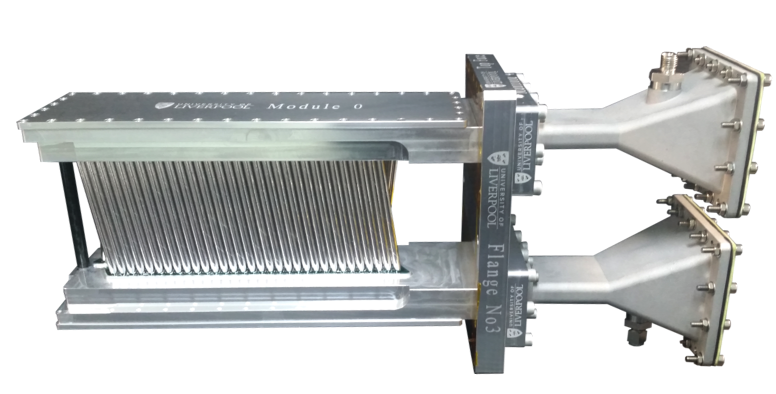
\includegraphics[width=0.9\textwidth]{Tracker}
\label{fig:tracker}
\end{figure}

\begin{figure}[]
\caption{Tracker modules are arranged in the shown staircase pattern. In green and dark blue is the edge of the vacuum chamber (where the dark blue identifies the modification that was made to the old vacuum chambers), and it can be seen that vacuum chamber walls lie at the ends of the outside tracking modules. The position of a calorimeter can be seen in teal at the right. The dark red spots are the locations of the pole tips.}
\centering
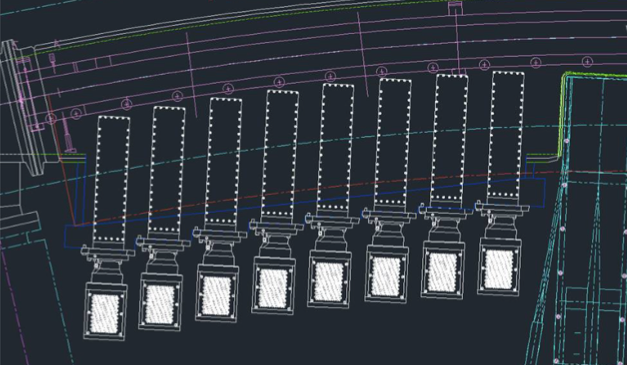
\includegraphics[width=0.9\textwidth]{trackerStation}
\label{fig:staircase}
\end{figure}


  Because of the proximity of the trackers to the muon beam, they will lie within a region of varying field. The radial field of the trackers rises from 0 Tesla at the outer ends to roughly .3 Tesla at the inner top and bottom ends, and the vertical field drops approximately 50\% from the storage dipole field of 1.451 Tesla. Shown in Figures \ref{fig:operaBy} and \ref{fig:operaBx} is the location of the tracker with respect to the horizontal and vertical fields respectively. If one thing can be said to be special to g-2 when it comes to tracking it is these large field gradients over the tracking detector region and several meter long extrapolation distance back to the muon decay point. This is one of the main motivations for using the Geane (Geometry and Error Propagation) fitting algorithm and routines, which has direct access to the field. 


\begin{figure}[]
\caption{Shown is the vertical field of the g-2 magnet in and around the storage region as calculated in Opera 2D. The center of the storage region lies at 7.112 m along the x axis. The black box shows the rough location of the tracker with respect to the field (size exaggerated slightly). It can be seen that there is a large inhomogeneity within the tracker space, goring from left to right.}
\centering
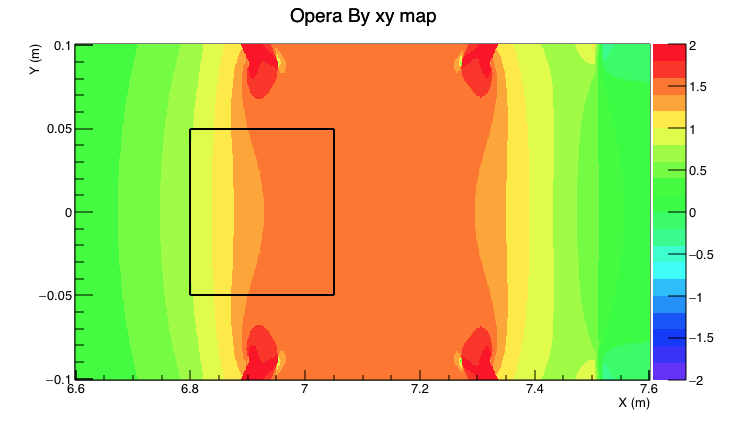
\includegraphics[width=0.9\textwidth]{operaBy}
\label{fig:operaBy}
\end{figure}

\begin{figure}[]
\caption{Shown is the radial field of the g-2 magnet in and around the storage region as calculated in Opera 2D. The center of the storage region lies at 7.112 m along the x axis. The black box shows the rough location of the tracker with respect to the field (size exaggerated slightly). It can be seen that there is a large homogeneity at the inner upper and lower ends compared to the right center. The shape of the pole pieces and tips can readily be seen.}
\centering
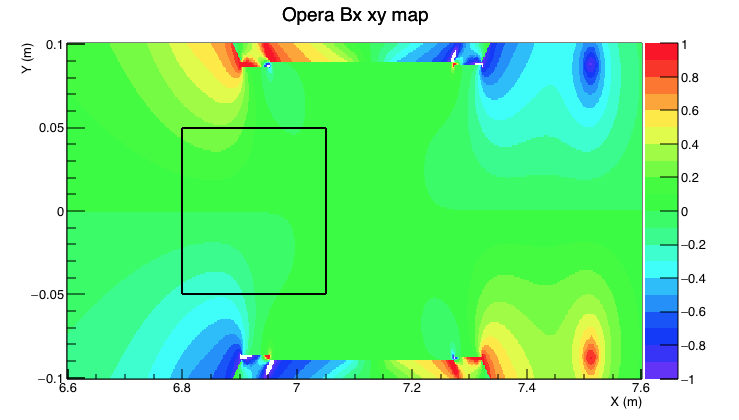
\includegraphics[width=0.9\textwidth]{operaBx}
\label{fig:operaBx}
\end{figure}

  The Geane fitting routines originated in Fortran with the EMC collaboration, and was used in the precursor E821 experiment as well as the PANDA experiment with some success. (cite stuff here?) (There might be some other instances of its use as well.) The core error propagation routines were at some point added to Geant4 under the error\_propagation directory which is included in all default installs. The tracking code strengths lie with its direct implementation and access to the Geant4 geometry and field, and its ability to handle the field inhomogeneties. The Geane algorithm code which makes use of the Geant4 error\_propagation routines follows the structure of \cite{geanemanual} and is detailed in the \hyperref[sec:Formalism]{Formalism} section in this paper. It is a relatively straight forward least squares global $\chi^{2}$ minimization algorithm. 



\section{Formalism}
\label{sec:Formalism}

    I recommend reading \cite{geanemanual}, Chapter 4 of \cite{Lavezzi}, and \cite{trajfit} in order to best understand the fitting algorithm. However, due to the at times confusing notation, ommitted equations or concepts, and differences between papers, I have attempted to summarize here the different sources and present the material in a more understandable and readable format. The implementation of the fitting algorithm into the code follows this section.

    One can define a $\chi^{2}$ for a track in the usual way by dividing the residuals of measured and predicted track parameters by their errors:
        \begin{align} \label{eq:chi2}
            \chi^2 = (\vec{p}-\vec{x})^{T} (\sigma^{-1}) (\vec{p}-\vec{x}),
        \end{align}
    where $\vec{p}$ are predicted track parameters from a fit to the measured track parameters $\vec{x}$, and $\sigma$ is a covariance matrix of errors on the fitted parameters. The Geant4 error propagation routines can be used to determine these predicted parameters and error matrices by propagating track parameters from some initial guesses. By minimizing this $\chi^{2}$ with respect to the track parameters one can then fit and improve the track. The Geant4 error propagation routines propagate particles along their average trajectories neglecting the effects of discrete processes, using a helix equation along small enough steps where the change in the magnetic field is small. The predicted parameters are then a function of path length: 
        \begin{align} \label{eq:pp}
            p_{l} = F_{l,l_{0}}(p_{0}),
        \end{align}
    where the path length can be defined how one wishes. In our system we have tracker planes defined at X positions, and limit path lengths to reach those planes. (From here on the dependence on path length or X position will be neglected, in favor of using plane indices.) In tandem, error matrices describing the expected distribution in true parameters about those predicted parameters due to said discrete process are also calculated:
        \begin{align} \label{eq:sigma}
            \sigma^{ij} = <p^{i}p^{j}> - <p^{i}> \cdot <p^{j}>,
        \end{align} 
    where i and j are track parameter indices. These parameter vectors are 5x1 objects defined in some track representation, as described in the \hyperref[sec:Coord]{Coordinate Systems} section. The propagation of these parameters and error matrices are done using transport matrices, which express the infinitesimal changes in parameters at some plane (or path length) with respect to the parameters at some previous plane (or previous path length):
        \begin{align} \label{eq:transport}
            \delta p_{N} = T_{N,N-1} \delta p_{N-1}, \\
            \sigma_{N} = T_{N,N-1} \sigma_{N-1} T_{N,N-1}^{T}.
        \end{align}
    Said transport and error matrices are 5x5 objects since the parameter vectors are 5x1 objects as described above. The calculation of these transport matrices, as well as details on the functional form of \ref{eq:pp} are shown in \cite{jacob}.

    With parameters defined on such planes, one can define the $\chi^{2}$ as: 
        \begin{align} \label{eq:chi2sum}
            \chi^2 = \sum_{i=1}^{N} [(p_{i}(p)-x_{i})^{T} (\sigma_{i}^{-1}) (p_{i}(p)-x_{i})],
        \end{align}
    where $p_{i}$ are the average predicted parameters from some general starting parameters $p$. At first order one can solely include the measurement errors on parameters, which fill in the diagonals of $\sigma_{i}$, if random processes can be neglected. Unmeasured parameters should have measurement errors of infinity (or some large value) along the diagonals in the code, which account for the fact that residuals for unmeasured parameters do not exist. When the error matrix is inverted all rows and columns of the matrix with these large numbers will fall to 0 in the $\chi^{2}$. 

    In order to get the best fit track, the $\chi^{2}$ should be minimized with respect to the initial track parameters p, and evaluated at some chosen or fitted parameters:
        \begin{align} \label{eq:minimize}
            \frac{\partial \chi^{2}}{\partial p}|_{p=p'_{0}} = 0,
        \end{align}
    resulting in
        \begin{equation}
        \begin{aligned}
            0 = \sum_{i=1}^{N}[ (\frac{\partial p_{i}(p)}{\partial p}|_{p=p'_{0}})^{T} (\sigma_{i}^{-1}) (p_{i}(p'_{0})-x_{i}) \\ 
            + (p_{i}(p'_{0})-x_{i})^{T} \frac{\partial(\sigma_{i}^{-1})}{\partial p}|_{p=p'_{0}} (p_{i}(p'_{0})-x_{i}) \\ 
            +  (p_{i}(p'_{0})-x_{i})^{T} (\sigma_{i}^{-1}) (\frac{\partial p_{i}(p)}{\partial p}|_{p=p'_{0}})]
        \end{aligned}
        \end{equation}
    where the 1st and 3rd terms are identical, and the 2nd term is small if one assumes that the error matrix doesn't change much with respect to the starting parameters. (Fair since most of the error comes from measurement, and as long as the initial guess is decent enough such that the path length through material doesn't change appreciably from one iteration to the next.) This simplifies to: 
        \begin{align} \label{eq:solve}
            \sum_{i=1}^{N} T^{T}_{i0} (\sigma_{i}^{-1}) (p_{i}(p'_{0})-x_{i}) = 0,
        \end{align}
    which is just the top term with 
        \begin{align} \label{eq:transport2}
             T_{i0} = \frac{\partial p_{i}(p)}{\partial p}.
        \end{align}
    To solve this make the substitution 
        \begin{align} \label{eq:psub}
            p_{i}(p'_{0}) = p_{i}(p_{0}) + \frac{\partial p_{i}(p_{0})}{\partial p} \Delta p_{0} = p_{i}(p_{0}) + T_{i0} \Delta p_{0},
        \end{align}
    where $p'_{0}$ are the improved starting parameters for the next iteration calculated from the previous starting parameters $p_{0}$, and $\Delta p_{0}$ are the changes in the starting parameters to improve the track. This equation can be plugged into the above if one makes the assumption that $T_{i0}$ does not change much from one iteration the next, which follows from the inherent nature of making small adjustments to the track in order to improve it.

    After simplifying one arrives at 
        \begin{align} \label{eq:deltap}
            \Delta p_{0} = \sigma_{p_{0}} \sum_{i=1}^{N} T^{T}_{i0}(\sigma_{i}^{-1})(x_{i} - p_{i}(p_{0})),
        \end{align}
    where
        \begin{align} \label{eq:cov}
            \sigma_{p_{0}} = [\sum_{i=1}^{N} T^{T}_{i0} (\sigma_{i}^{-1}) T_{i0} ]^{-1},
        \end{align}
    is the 5x5 covariance matrix of fitted parameters on the starting plane, whose diagonals describe the errors in the 5 track parameters on that plane and in the region close to it. (The fit does not directly return fit errors for track parameters on other planes.) $\Delta p_{0}$ along with $\chi^2$ is exactly what we want to determine since that is what allows us to fit and improve the track from iteration to iteration.

    However, since random processes should not be neglected for optimal tracking results, it makes more sense to return to the original $\chi^2$ in equation \ref{eq:chi2}, only now the included matrix and vector objects are combined into one large linear algebra equation. Instead of a sum over N 5x1 objects multiplying 5x5 error matrices, the vectors are combined into a single 5Nx1 vector multiplying a single 5Nx5N matrix. The 5x5 diagonal blocks of this large error matrix should now include the effects due to material processes as calculated in Geant from equation \ref{eq:sigma} as well as the measurement errors. 

    Because now parameters at one plane are no longer independent of the parameters at other planes, due to correlations from these random processes, it's necessary to add off-diagonal elements into the large error matrix. These 5x5 blocks come from 
        \begin{align} \label{eq:corr}
            \sigma_{MN} = T_{MN} \sigma_{N}, 
        \end{align}
    for the top diagonals, and the transpose for the bottom diagaonals, where M and N are two separate planes within the detector. ($\sigma_{N}$ is the error matrix on plane N calculated from the starting plane.) This follows from equation \ref{eq:sigma} evaluated at plane M with respect to a path length from plane N, and not plane 0, which is equivalent to \ref{eq:corr}. 

    You can then minimize the $\chi^{2}$ in the same way, only again with the matrix objects being aggregates of the per plane objects:
        \begin{align} \label{eq:deltafull}
            \Delta \vec{p}_{0} = \sigma_{p_{0}} \tau^{T}\sigma^{-1}(\vec{x}-\vec{p}),
        \end{align}
        %
        \begin{align} \label{eq:covfull}
            \sigma_{p_{0}} = [\tau^{T} \sigma^{-1} \tau ]^{-1},
        \end{align}
    where $\tau$ is the combined transport matrices from the individual 5x5 matrices, a 5Nx5 object.

    The unmeasured parameter errors of infinity still come into play in the final calculation in the same was as before. Because however these matrix objects are very large, and the tracking must have a certain amount of speed in order to keep up with data, it is useful to reduce the size of these matrices. (It also makes things easier programming wise. Note that there are other some other ways to speed things up, specifically the banded inversion method as described in reference \cite{trajfit}. This method was not used in favor of getting the code working in the simpler form in the first place, but it is a possiblity in the future to use this technique to speed things up even more.) It suffices to simply remove all rows and columns where said infinity values exist in the error matrix. This is mathematically equivalent to inverting the error matrix with the infinities included, which make all rows and columns where they exist go to zero. The associated unmeasured parameter rows in the residual vector and transport matrices must similarly be removed. This results in an Nx1 residual vector, NxN error matrix, 5xN combined transport matrix transpose, which multiply against the 5x5 covariance matrix out front to still result in a 5x1 fix to the starting parameters, and a scalar $\chi^2$ value. (Note that these element removals should be done just before the final calculation, and not higher up in the algrebra, otherwise plane correlations are not properly calculated.)

    By calculating the last two equations one can fit the track, acquire a $\chi^{2}$ describing the degree of the fit, determine how the track parameters can be improved at the starting point, and calculate errors on those starting parameters. This algorithm can be iterated a number of times to get a best fit track until successive iterations produce no improvement, where usually 3 or 4 iterations is enough. Note that there is remarkable robustness with respect to the initial starting parameters in fitting the track. Of course if the initial starting paramaters are too poor, then the fit will not converge. All of these calculations are completed within the \hyperref[sec:GeaneFitter]{GeaneFitter.cc} file within the framework.
 % Math stuff

\section{In the gm2 Framework}
\label{sec:Framework}

  Depending on the level to which a user wants to utilize or develop the tracking code, they may choose which branches of the gm2 framework to checkout. If just fitting tracks and viewing plots, then just gm2tracker on the develop branch may be checked out. If doing further development, it can be a good idea to checkout the artg4, gm2dataproducts, gm2geom, gm2ringsim, gm2tracker, and gm2utils packages of the gm2 repository, and be on the feature/trackDevelop branch in all instances. Every so often these branches are merged with the main develop branches, where the tracking code will work but might not have the latest code changes. 

  \subsection{Event Generation, Geometry, and Material}

    While not a direct part of the reconstruction and fitting code, there is relevant information with respect to event generation in the simulation upon which the reconstruction acts. Event generation before fitting is done using the mdc fcl files in gm2ringsim using the main simulation, where one can also include the tracker dummy plane geometry for truth comparison with the Geane fitting if so desired. These are built in the TrackerDummyPlane\_service and associated geometry files, and are included in the common mdc fcl files. If one wishes there are also a couple of modified mdc\#-geane fcl files available for use with reduced geometry. For stats reasons it is usually a good idea to include all 3 trackers when generating events.

    Fcl parameters exist for the StrawTrackerCadMesh\_service and Straws\_service in order to turn material on or off at will, ``materialTracker'' and ``strawMaterial'' respectively. The rest of the geometry has to be manually changed and rebuilt in order to remove material if one wishes. These include VacuumChamberCadMesh and the World, as well as the ``buildSupportPost'' option in strawtracker.fcl, ``buildTrolly'' in vac.fcl (where the associated material is hardcoded in), and ``trolleySupportMaterial,'' also in vac.fcl. One should make sure to perform reconstruction with the same material parameters as were used in the event generation for proper results. (These options are primarily for debugging the tracking. Near perfect results have been shown for tracking within a vacuum world, \href{http://gm2-docdb.fnal.gov:8080/cgi-bin/ShowDocument?docid=4876}{DocDB 4876} and \href{http://gm2-docdb.fnal.gov:8080/cgi-bin/ShowDocument?docid=4894}{DocDB 4894}.)


  \subsection{Reconstruction Flow}

    The overall tracking infrastructure and reconstruction flow can be seen in Figure \ref{fig:Infrastructure}. Data coming from simulation or the real experiment, are turned into art objects upon which the tracking framework acts. The RunGeane.fcl file (detailed more below) performs the entire chain within the blue box in Figure \ref{fig:Infrastructure}, excepting the track extrapolation stage. Within the reconstruction flow objects called Track Candidates are produced, which are the input to the Geane fitting code.


\begin{figure}[]
\caption{Shown is the infrastructure flow for the entire track reconstruction chain. In the green blocks are the sources of track data to fit, either from Geant simulation, or real data. In blue is the offline reconstruction block. Straw digits are formed in the digitalization step, those are then calibrated and grouped into time islands, clusters, and seeds which then combine to form track candidates. It is these track candidates which are the input into the Geane fitting code (and other future fitting code). The fitting code then outputs tracks which the track extrapolation stage will run over. This picture is taken from one of Tammy's talks. Note that there is some iteration here that is not shown.}
\centering
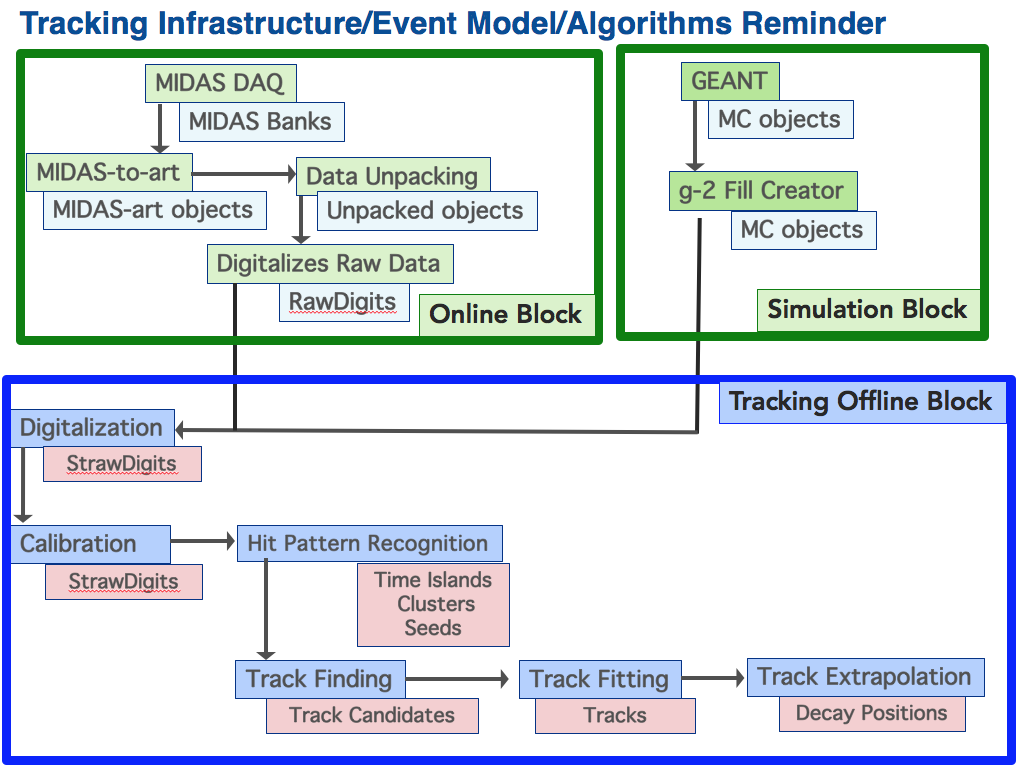
\includegraphics[width=0.9\textwidth]{TrackInfrastructure}
\label{fig:Infrastructure}
\end{figure}

\begin{figure}[]
\caption{Shown is the Geane fitting code flow. See the text for a thorough explanation of this flow, and the specifics of each box. GEANEArtRecords are created in the GeaneReco producer module, and are passed by pointer and reference to the different utils files which then updates them for the different fitting modes and with the fitting results.}
\centering
\hspace{15mm}
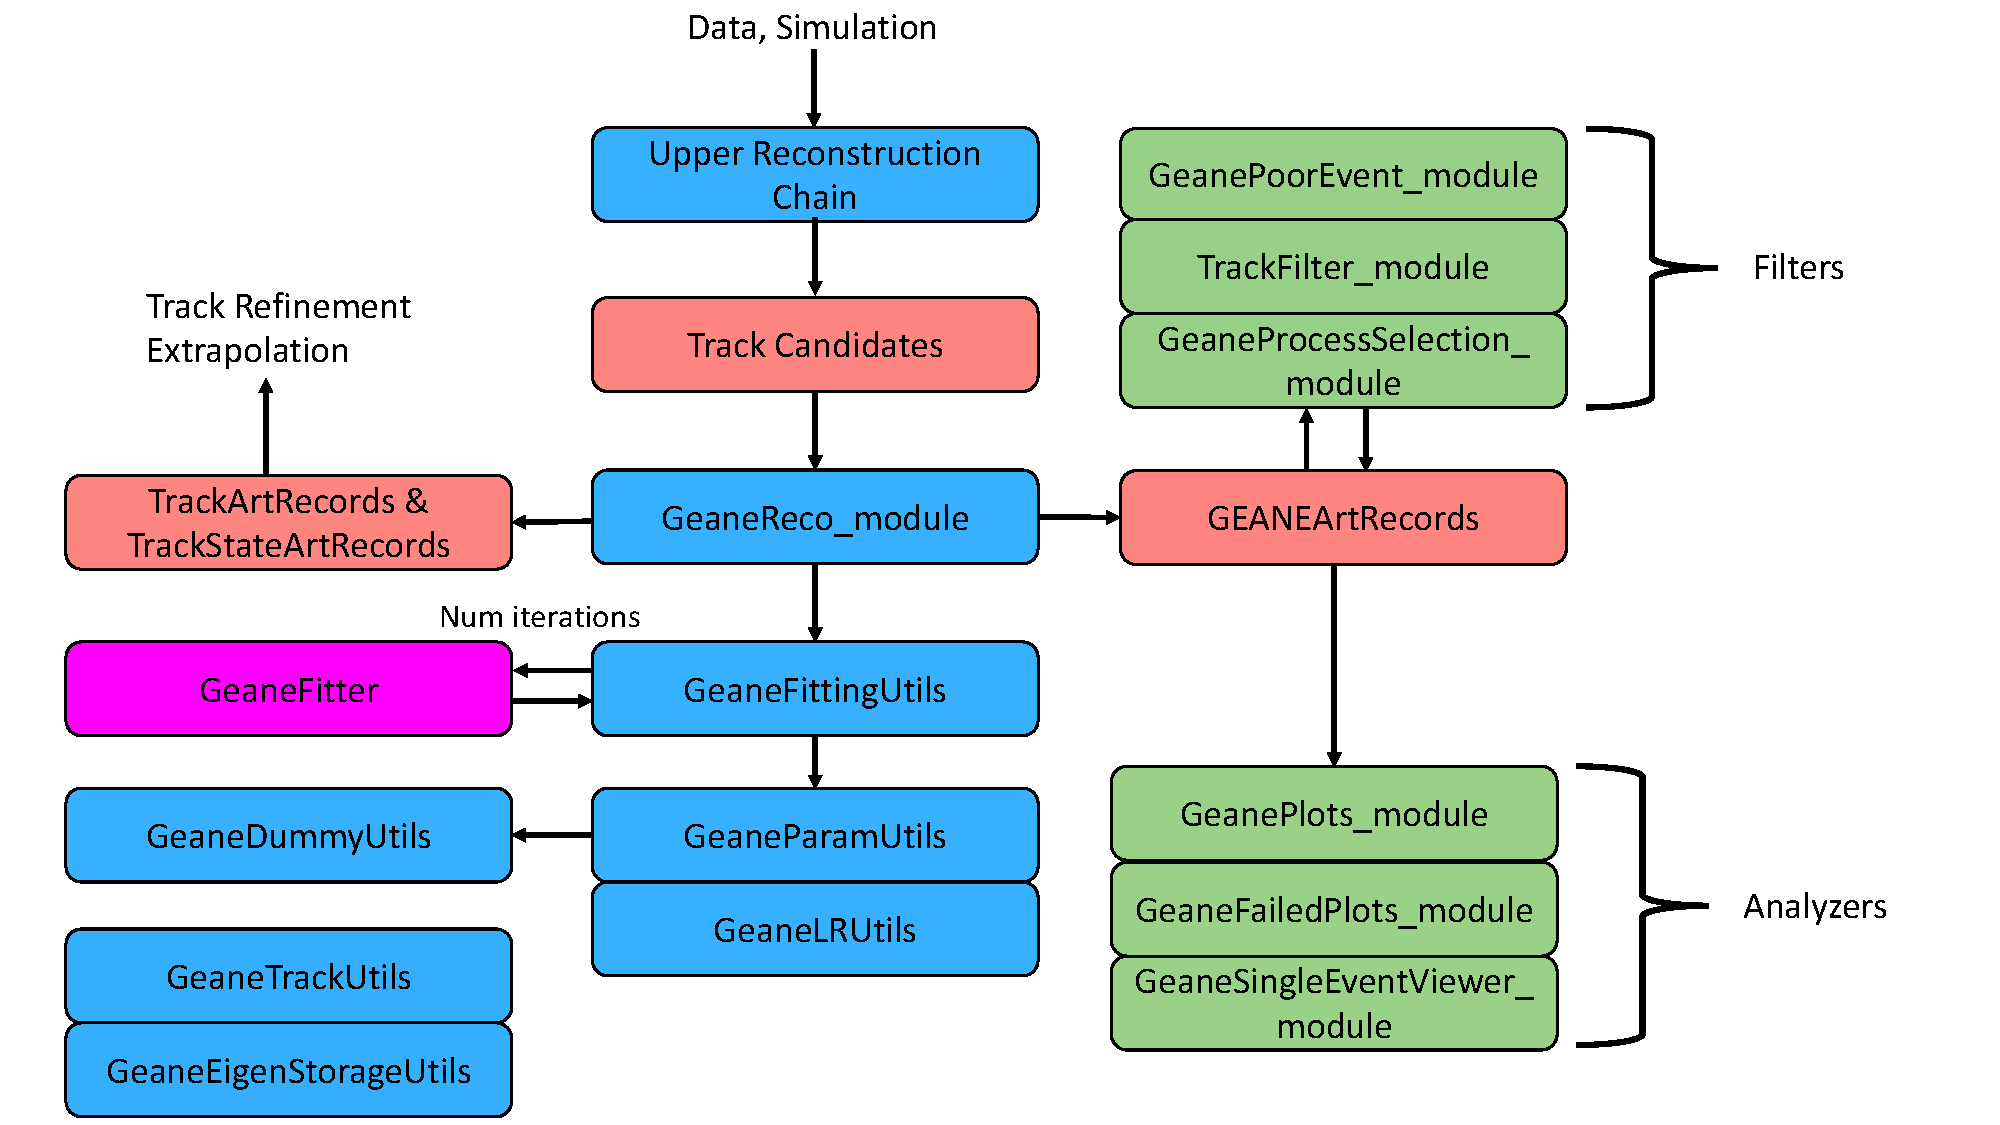
\includegraphics[width=0.9\textwidth]{NewGeaneFlow}
\label{fig:NewGeaneFlow}
\end{figure}


    The Geane fitting specific flow can be seen in Figure \ref{fig:NewGeaneFlow}. There is a number of files involved in the production of fitted tracks. Detailed information regarding all of these files is given below, but here is provided a shorter summary. Track candidates from upstream are used as the input to the producer module GeaneReco, which produces TrackArtRecords and TrackStateArtRecords, which are then passed to the extrapolation or refinement stage. GeaneReco also produces GEANEArtRecords, which is the data product that is used and updated throughout the fitting process until the track converges or fails, and may be passed through filters or to analyzers at the end of the fitting. There are a number of utils files that the Geane fitting utilizes. GeaneReco directly links to the GeaneFittingUtils which contains a number of methods for the different fitting modes, as well as the general fitting loop which links to the GeaneFitter class, and iterates until the track fitting succeeds or fails. GeaneFitter provides a $\chi^{2}$ and improvement to the track as described in the \hyperref[sec:Formalism]{Formalism} section. GeaneFittingUtils links to GeaneParamUtils and GeaneLRUtils. GeaneParamUtils deals with any code that modifies parameters regarding the fit, both setting up the initial fit parameters, and calculating the predicted parameters of the fit within Geant4 using the error\_propagation routines. GeaneLRUtils deals with any code regarding the left and right information of the track for fitting.
    
    Note that after a single iteration, one pass through GeaneFitter and one pass through the relevant fitting utils, a $\chi^{2}$ and an improvement for the track will be produced, but the track predicted parameters and objects will be based on the previous starting position and momentum guess before it has been updated, and so do not correspond to the fitted track. It's necessary to perform at least a second iteration for this reason, and is why no track converges under the strict criteria in under 3 iterations.

    Also worth mentioning is that the GEANEArtRecords are passed by reference or pointer throughout the various fitting files, allowing them to be updated along the way in a natural manner. At the same time, many methods within the fitting code return ints describing whether the track fitting has failed at different stages to various reasons, where a value of 0 signifies success at that stage. A returned int with a non-zero value might for example signify that too many digits were included in the initial track candidate, or that Geant is having tracking issues, etc.


  \subsection{fcl File Specifics - RunGeane.fcl} 
  \label{sec:RunGeane}

    Reconstruction is performed using RunGeane.fcl in gm2tracker on the events generated from somewhere higher in the chain. (There is also a RunGeane-midasdata.fcl file which is more tuned to running on real data, with certain fcl parameters set appropriately and some modules left out of the chain.) It is important to explain some fcl parameters necessary for the reconstruction. First, there is a fcl parameter ``useSD'' for the Straws geometry service to turn off the straw sensitive detectors so that in the reconstruction phase hits are not regenerated. If this is not included, it will default to true and cause crashes in the reconstruction. Secondly, the RunGeane.fcl file loads all 3 trackers necessary for symbol and name definitions, but such that tracker 0 is rotated such that the tracking planes are parallel to the global geant X axis (using the rotateArcTracker fcl parameter for the Arc service). This is done to avoid the issue of error propagation instability close to the Z axis, as detailed in \href{http://gm2-docdb.fnal.gov:8080/cgi-bin/ShowDocument?docid=4567}{DocDB 4567}, while at the same time still observing the correct azimuthally symmetric 2D field for the tracks. Track hits are rotated from their separate tracker frames to this one reconstruction frame with the GeaneWorldTracker[0], GeaneWorldTracker[12], and GeaneWorldTracker[18] transforms defined at the bottom of StrawTrackerCadMesh\_service.cc, and as detailed in the \hyperref[sec:Coord]{Coordinate Systems} section. (In the future, if fields or geometries are not identical between trackers, the details here will have to be improved after changes have been made.) As a reminder there are material fcl parameters for the straws and straw trackers which should be the same as were used in the event generation. The RunGeane.fcl file also includes some analyzer and filter modules by default, which are detailed further below, and can be turned on and off at will.

    While the pieces of the chain before the track fitting (digitalizing, seeding, clustering, t0 finder, and track finding) are distinct and separate from the material detailed in this document, it is important to understand at some level those stages and the different options which will affect the tracking results. See a collaboration talk by Tammy, \href{http://gm2-docdb.fnal.gov:8080/cgi-bin/ShowDocument?docid=5601}{DocDB 5601}, for a general overview on this. Here is a short summary, not all method or file calls are detailed. Most of these files and parameters should be left unchanged unless one is familiar with the subject matter.

    \begin{enumerate}

          \item{\bf{Digitalizer\_module.cc}} \\
          This module creates StrawDigits which will ultimately be combined to form the Track Candidates that the fitting will act over. It is the variables in this art record that are updated and correspond to real data, which straw was hit, the time of the hit, and the dca of the hit. The StrawDigits also contain a pointer to a struct of Monte-Carlo truth data, StrawMCDigit, which can also be accessed for track information. The Digitalizer module has several fcl parameters to change things like the gas drift time, drift model, allowing recorded negative times, and some particle cuts. By default it uses a Gaussian drift model which is called when the Digitalizer calls the DriftTimeModels.cc file, where it will gaussian smear the hit time from the MC digit time. These fcl parameters are located in digitalizerParams.fcl. The smearedDriftTimeSeed parameter should be set to 0 if one wants random results from run to run, which is necessary for grid jobs. The drift time model can also be set to the Garfield version, which will produce more realistic measurement parameters. If this is used the drift time calculator in the DriftDistanceCal module should also be set to the Garfield version. These more realistic hit data result in reconstructed tracks that haven't been fully analyzed yet, with a non-uniform p value distribution.

          \item{\bf{TimeIsland\_module.cc}} \\
          Groups the digits from the Digitalizer in time. Has some options for changing the time window width. fcl parameters are located in recoIslandParams.fcl. There is ongoing work in relation to this module for dealing with real data, where there is a much increased number of hits closer in time. The short summary here does not reflect the difficult and important task that this module has.

          \item{\bf{ClusterFormation\_module.cc}} \\
          Groups neighboring digits in the same view to form clusters. fcl parameters are located in recoClusterParams.fcl.

          \item{\bf{T0Finder\_module.cc}} \\
          Calculates a t0 for the track. Has an option for which model to use for calculating said t0. The default is using truthData if one is running the tracking over simulated hits. If one is looking at real data there are other options. It's important to note that the t0 for a track can be difficult to calculate, and the current goal is to combine information from the calorimeter to get this number. fcl parameters are located in recoT0FindingParams.fcl.

          \item{\bf{DriftDistanceCal\_module.cc}} \\
          Calculates the drift times and distances within the straws based on the calculated t0 from the previous module. Has options for different drift calculators and parameters, including a ``useTrueDigitT0'' parameter for using mc truth information. The drift time is calculated from the digit hit time (calculated in the Digitalizer) minus the digit t0. If true t0 is not used, then the dca smearing will not be perfectly gaussian. fcl parameters are located in recoClusterParams.fcl.

          \item{\bf{SeedFormation\_module.cc}} \\
          Groups neighboring clusters in the same module to form seeds. There are two fcl parameters for this module. The first is ``reconstructPosition'' which will fill seed nodes which form the seed, and essentially correspond to indidual digits - but which contain some left-right (LR) ambiguity information important for track fitting. The second is ``useGeometryLR'' which uses the straw geometry information to make an initial guess at the left-right choices for doublets within the track. fcl parameters are located in recoSeedParams.fcl.

          \item{\bf{Aside}}
          It's important to note that there is another iteration of the clustering module which is improved now that better drift times and distances have been calculated from the previous modules, using the same fcl paramters. This will almost certainly change in the future as the tracking code becomes more developed.

          \item{\bf{TrackFinding\_module.cc}} \\
          Groups time islands and digits based on their positions in space. There are two finders available for use, fcl parameter trackFinderName, the Simple Track Finder (SimpleTrackFindingUtils.cc) and the Long Track Finder (LongTrackFindingUtils.cc). The former just runs off the generated time islands. If you use this, then the second clustering module and seed formation module can be left out of the reconstruction chain. The latter, Long Track Finder, forms track candidates based on combining seeds and is the default used. It also has stricter fcl conditions, such as a default cut of 6 or more planes hit for the track. Both finders make use of the SimpleCircleFitter.cc class which fits a circle to the U and V digit positions to calculate a starting position and momentum guess for the track, which is currently necessary for the Geane fitting. The Long Track Finder also has a least squares minimizer which is unimportant for the Geane fitting. fcl parameters are located in recoFindingParams.fcl, which then also links to some other fcl files depending on the finder used.


    \end{enumerate}

  \subsection{geaneFitParams.fcl}

    Because the Geane track fitting is the subject of this document, it will go more into detail of the Geane fitter fcl parameters, located in the geaneFitParams.fcl file. Some of these parameters are very likely to change or disappear in the near future.

    \begin{enumerate}

      \item{\bf{module\_type}} \\
      The ordinary art producer parameter which tells art which cc file to run, this is always set to GeaneReco unless the filename changes.

      \item{\bf{G4EVERBOSE}} \\
      This parameter corresponds to the iverbose level present in the Geant4 error\_propagation files and can be manually set here, from 0 to 5. It is for the debugging of deeper level Geane fitting code. Note that unless Geant is compiled with the flag by the same name setting this verbose level will do nothing. Since currently we utilize our own slightly modified error\_propagation files copied into the gm2tracker/gm2Geane directory, it would be possible to remove the dependencies on this Geant4 build flag. Since however this will slow down the tracking it is the current choice to leave them in. 

      \item{\bf{trackingVerbose}} \\
      Geant4 tracking verbose level, from 0 to 5. This is always available but should only be used for debugging.

      \item{\bf{matrixDebug}} \\
      This boolean paramater turns on and off the copious matrix debugging output, used for deep level debugging. Note that these outputs are included in the log file and the log file threshold needs to be set to ``DEBUG''. In the future it might be beneficial for speed reasons to remove completely these debugging outputs. This parameter should always be turned off if looking at a large number of events.

      \item{\bf{numPassesWireFit, numPassesSeqFit}} \\
      These are parameters used for the Left-Right sequence checking routines for a full fit. numPassesWireFit is the number of passes that the track should be fit to the wire centers, before which the best sequences were passed to the main fit code which would iterate a number of times equal to numPassesSeqFit. It was observed in the past that 3 passes for each of these was sufficient for good tracking results. 

      \item{\bf{convergenceCriteria}} \\
      This is a scalar convergence criteria telling whether the track fitting has been successful or not, with a default value of .1. As long as the current iteration $\chi^{2}$ minus the previous iteration $\chi^{2}$ is less than this value, the track is considered to have converged, otherwise it continues iterating until it succeeds, fails, or is manually cut off at 10 iterations.

      \item{\bf{useCircleGuess}} \\
      This boolean parameter tells the code whether to use the circle fitter results for the track starting guess or not, called in the track finding part of the chain. It's default should remain true unless one wants to return to the uniform starting parameter smearing for debugging purposes.

      \item{\bf{lockLowDCAs}} \\
      This is a temporary fcl parameter which will take measured hits with small dcas and set the measured positions to the wire centers, at the same time locking the LR choices to the center. This will be necessary when fitting data due to the large measurement uncertainty of hits close to the wire, and at the same time speeds up the code with less LR choices to iterate over. It's default value of 0 corresponds to turning this functionality off, while a positive number corresponds to the radius in mm that dcas less than will be locked.

      \item{\bf{useNodes}} \\
      This boolean parameter sets whether to use the left-right information from the seed nodes, if activated. The recoSeedParams fcl parameter ``reconstructPosition'' needs to be set to true for this to work, and the parameter ``useGeometryLR'' should also be set to true, being that it is the only upstream left-right code currently implemented.

      \item{\bf{fitMode}} \\
      This is the most important fcl parameter for the Geane fitting. It defines what type of fitting mode you'd like to use for fitting the incoming track candidates. There are currently 4 separate fitting modes. ``truthLRFit'' only works with simulated data and will fit to the unambiguous LR UV values from the digits. ``wireFit'' will fit a track to the wire centers of the incoming digits, with a corresponding uniform error proportional to the gas diameter. ``mainFit'' will first do a wire fit to the track in order to make an initial guess at the LR choices for each hit, and will then fit to those LR choices. (The default main fit actually does a second wire fit in the middle where it first locks LR choices for doublets where the LR choice is guaranteed to be known, which improves the tracking results slightly.) Finally there is the ``fullSeqFit'' which will first do the wire fit, and will then go about checking all LR sequences before doing full fits on the set of best sequences. (There is also some code to lock the left-right sides based on the doublets.) This LR procedure is detailed lower in this document.

      \item{\bf{useTangentLR}} \\
      This fcl parameter links to code which does a slightly more advanced locking of the doublet left-right geometry include track tangent information, defaulted to false, and written by Joe Price.

      \item{\bf{rseed, yPosChange, zPosChange, xMomChange, yMomChange, zMomChange}} \\
      These are the uniform smearing bounds for the starting position and momentum of the track from truth, units of mm and MeV. These are largely unused now since the circle fitter provides a level of smearing automatically when it's used, but should be kept for future debugging purposes. The rseed parameter is the number seed for the random number generator. The default should be 0 for the root TRandoms unless one wants to reproduce results.

    \end{enumerate}


  \subsection{Reconstruction Files}

    Here will be given a summary of the different core files used in the Geane track fitting as shown in Figure \ref{fig:NewGeaneFlow} and explained up above, as well as extensive detail where necessary. 


    \begin{enumerate}

      \item{\bf{GeaneReco\_module.cc}} \\
      This file is the producer module for the track fitting reconstruction. It pulls in upstream data products, TrackCandidateArtRecords, and produces TrackArtRecords, TrackStateArtRecords, and GEANEArtRecords. The GEANEArtRecords are what's passed through the various fitting utils files until the track fitting succeeds or fails, and from which the TrackArtRecords and TrackStateArtRecords are derived from. GeaneReco directly links to GeaneFittingUtils where the track fitting is actually done.

      \underline{Methods}

        \begin{itemize}

          \item{\bf{produce}} \\
          General overriden produce method. Calls main track fitting code on an event by event basis. Produces data products for downstream use.

          \item{\bf{trackFitting}} \\ 
          Short method which first calls down through GeaneFittingUtils into GeaneParamUtils to set up the initial parameters for fitting, and then calls the method corresponding to the particular fit mode specified in the fcl file. Also has a method call for checking some failure modes after fitting.

        \end{itemize}

      \item{\bf{GeaneFittingUtils.cc}} \\
      \label{sec:GeaneFittingUtils}
      This class contains several methods for fitting tracks with different fit modes. Each such method sets up the specifics of the fit, altering necessary parameters and calling various methods, and then calling the fittingLoop method which iterates and fits the track. mainFit and fullSeqFit do multiple fits, starting with a wire fit. 

      \underline{Methods}

        \begin{itemize}

          \item{\bf{truthLRFit}} \\
          Fits a track to the U and V hits with the left-right sides known from the Monte Carlo simulation. Only works with simulation.

          \item{\bf{wireFit}} \\
          Fits a track to the wire centers of the hit straws, ignoring left-right information. This is the easiest fit to do on data since it ignores timing information, which affects dca values and errors.

          \item{\bf{mainFit}} \\
          First does a wire fit to the track in order to gain left-right information, then does a hybrid wire fit with some left-right choices set based on the doublet geometry and predicted parameters from the first wire fit. Finally fits a track to the dca values of the hits with the left-right sides set from the previous fit, updating each iteration.

          \item{\bf{fullSeqFit}} \\
          First does a wire fit to the track in order to gain information useful for solving for the left-right sides of the track. Then locks left-right sides based on used fcl parameters, and sets associated errors, leaving the remaining sides as ``unknown.'' Then does a fast check or approximate fit on all U and V unknowns separately in order to determine a set of best possible U and V left-right combinations. Finally takes the best U and V left-right combinations and combines them into full left-right sequences, which are then fitted as normal with the associated dcas and errors. See the \hyperref[sec:LR]{Left-Right} section for more detail on this.

          \item{\bf{fittingLoop}} \\ 
          The general fitting iteration loop method. Takes in the GEANEArtRecord, the number of passes to fit over, and whether to update the left-right sides each iteration (for mainFit) as parameters. For each loop it will calculate the predicted parameters and propagate the errors of the fit by calling the errorProp method within GeaneParamUtils, then update the left-right sides from the previous iteration if desired, then calculate the angle-corrected measured parameters based on the left-right sides of the track to fit. Finally, with all parameters determined, it will calculate a $\chi^{2}$ and an improvement for the track by calling the TrackCorrelation method from the class GeaneFitter. The improvement to the track from GeaneFitter serves as the basis for calculating the next set of predicted parameters. Relevant GEANEArtRecord members are filled and then the track is checked to have converged, with fittingLoop iterating if it has not. 

          \item{\bf{checkExtraneousFailureModes}} \\
          A mostly defunct method with the purpose of checking to see whether the tracking has failed in some unseen way. In the past there were some failure modes which have since been removed such as a track reconstructed with overly high momentum. Currently the only failure mode check is to see whether the X positions of the reconstructed track don't match the wire positions, which should not be the case since the former directly comes from the other. Some coordinate code which may be the root cause of this is commented out due to framework coding constraints (which can probably be gotten around). This method has been left in for the future possibility of checking other potential failure modes.

        \end{itemize}

      \item{\bf{GeaneFitter.cc}} \\
      This file consists of the main track fitting $\chi^{2}$ algorithm. It multiplies measured parameters, predicted parameters, error matrices, and transport matrices together to produce a chi2 for the track and an improvement to the starting paramters. It also reads in the measured hits errors in order to properly fit the track. See the \hyperref[sec:Formalism]{Formalism} section for a detailed description of what this class really does. There is a fcl parameter matrixDebug which can be used to turn on or off the many large matrix cout debugging statements.

        \begin{itemize}

          \item{\bf{TrackCorrelation}} \\
          The main matrix multiplication routines, essentially the math from reference \cite{geanemanual}. In order to fit the track properly with the correct errors, the matrix multiplication must be done in the XUV space. Since the transport matrices and predicted parameters are generated in the XYZ space as described in the errorProp method of the \hyperref[sec:GeaneParamUtils]{GeaneParamUtils} section, they must be converted using the Jacobian transformation between the two bases. This Jacobian is described in the \hyperref[sec:Coord]{Coordinate Systems} section, and the variable itself is saved as a member in the GeaneTrackUtils.cc class. 

          One other point of note regarding this method is that depending on the matrix multiplications being done, the various loops within the code might either loop over the maximum number of planes (33, a 0 plane plus the 32 measurement planes), or they might loop over the planes that were hit. The code should be relatively clear, but if any indices or loop iterators are messed up in any way, then the track fitting will utterly fail, sometimes with only very subtle hints as to where exactly the problem lies. (At one point I spent a week hunting down an off-by-one index error believing it to be a memory problem, due to how the Eigen matrices work.) At some point it might be beneficial to standardize this code, but it has been left alone per the reason stated before.

          \item{\bf{makeHybridErrMat}} \\
          A method in order to create a hybrid wire / U or V error matrix for the left-right sequence checking. Only called once per track for the U and V sequences.

          \item{\bf{sequenceChecking}} \\ 
          The main left-right sequence checking method for an individual event. This method is called up to thousands of times as each U or V sequence is checked. See the \hyperref[sec:GeaneLRUtils]{GeaneLRUtils.cc} and \hyperref[sec:LR]{Left-Right} sections further below for more detail on what this method does.

          \item{\bf{convertToGeVcm, convertToMeVmm}} \\
          Methods for converting Eigen 5 parameter vectors from GeV cm to MeV mm and vice versa.

        \end{itemize}

      \item{\bf{GeaneParamUtils.cc}} \\
      \label{sec:GeaneParamUtils}
      This file consists of the main methods which modify various parameters for the track fitting. The setupParams method does its namesake, setting up the initial parameters per track before attempting to fit. The errorProp method deals with calculating predicted parameters and associated track matrices within Geant4. Finally, the calcMeasuredParams method deals with setting and correcting the measured paramaters of the fit from the incoming dca values and errors of the track hits. Note that this is the only class in the Geane reconstruction framework which links to and uses Geant4. It is in the constructor of this method that the Geant4 world is constructed once per job, the proper magnetic field is associated with the transportation manager, and the error propagation routines are initialized. (The necessary Geant4, art service, and gm2geom header files are included here.)

      \underline{Methods}

        \begin{itemize}

          \item{\bf{setXPositions, setCoordMap}} \\
          Hacked in methods to grab needed coordinate system information and the X positions of the wire planes (from the art run object) while improving speed of the tracking.

          \item{\bf{setupParams}} \\
          This method sets up the parameters at the beginning of each track fit. It is here that the TrackCandidateArtRecord and StrawDigitArtRecord information is copied or converted into relevant GEANEArtRecord members. Other members are filled with default or empty values to start. Members include dcas, dca errors, wire positions, hit sides, etc. This method links to the GeaneDummyUtils file, which allows one to acquire the truth information of the track and use for fitting if desired. The starting guess for the position and momentum of the track can be pulled from the track candidate (calculated using a simple circle fitter to the hit digits) or truth. There are a couple of variables in the GEANEArtRecord which are filled with the same information in this method, as the initial setup is for doing a wire fit to the track. If doing a different kind of fit, the variable changes and method calls in GeaneFittingUtils handles altering the relevant parameters of the fit. There are also a couple of checks in this method to make sure that we're trying to fit a reasonable track, and not one that for instance has more than one hit on a measurement plane.

          \item{\bf{errorProp}} \\ 
          This method tracks particles along their average trajectories through the region of the tracker detector using the Geant4 error propagation routines with the correct geometry and field. It builds transport matrices, error matrices, and predicted parameters which are the objects used for fitting the track, as described in the \hyperref[sec:Formalism]{Formalism} section. It tracks on a plane by plane and step by step basis. These error propagation routines can be used to track particles forwards and backwards, where the forwards tracking is used in the code. (It will be non-trivial to change the code to be able to back-track.) 

          To be a little more explicit, it creates Geane free trajectory states which are the objects that are propageted from target plane to target plane, where the target planes are defined to be parallel in X. (As our wire planes are.) Surface trajectory states are then created on those planes, where the orthonormal vectors defining those planes are in the Y and Z directions. These vectors have to be orthornormal in Geant in order for predicted parameters and errors to be calculated correctly. It is later in the fitting code that these track objects are converted to the UV basis that our detector is naturally defined in. 
            
          While the predicted parameters and errors can be grabbed directly from the surface trajectory state on each plane, the transport matrix cannot be. It is on a step by step basis that the transport matrices are generated, with the previous step transport matrix being dropped with the next step. It is for this reason that the transport matrices must be accumulated and multiplied together from each step in order to form the transport matrix describing the change in parameters from one measurement plane to the next. (There is some code in the Geant source code which appears that might do this automatically, but it is commented out and unclear if it works.) These transport matrices are also only defined in the free state coordinate system, and so need to be converted to the surface system that our fitting uses. When creating surface trajectory states on the target planes, the Jacobian transformation matrices from the free to the surface system are generated and can be saved. It is then a simple matter of multiplying these matrices together to get the transport matrices in the surface system. (Once again these are defined in XYZ, but are converted later in the code to be in XUV.) See the \hyperref[sec:MatTransf]{Appendix} for details on these matrix transforms.

          It's also worth mentioning that within this method there are a number of checks to see whether the tracking has failed due to Geant stepping or Geane propagation issues.

          \item{\bf{calcMeasuredParams}} \\ 
          Method to correct measured parameters from a radial DCA value to a U or V value based on the momentum of the track at the hit from the previous fit and approximating a constant field within the straw. Also corrects the dca errors using a simple straight line approximation in a similar vein. See the \hyperref[sec:Appendix]{Appendix} section for more details on how this works. Note that this method also fills the measured parameter objects within the fit in the first place, so if this method is not called then the fit won't have any measured hits to fit to.

        \end{itemize}

      \item{\bf{GeaneDummyUtils.cc}} \\
      This class deals with truth track information, stored in GhostDetectorArtRecords generated by the TrackerDummyPlane service. These GhostDetectorArtRecords store position and momentum in the world coordinate system, and so need to be converted to the Geane coordinate system(s) when comparing the fitted track against truth or inputting any truth parameters into the fit. Called by GeaneParamUtils and some analyzers.

      \underline{Methods}

        \begin{itemize}

          \item{\bf{fillDummyHits}} \\
          Fills a local variable with the dummy hits from the art data handle, done once so that the utils file has access to the data products.

          \item{\bf{getTrackDummyHits}} \\
          Method to fill the GEANEArtRecord dummy hits member variable, dummyPlaneHits, with the ordered dummy hits corresponding to the hit measurement planes.

          \item{\bf{fillCS, fillStationStr}} \\
          Passes some needed coordinate system information to the utils file, and the station that the track was in for coordinate transforms to the correct frame.

          \item{\bf{fillDummyHitInfo, fillDigitHitInfo}} \\
          Fills some commonly used variables throughout different methods in the class.

          \item{\bf{fillTruthParams}} \\
          Brute force searches through the GhostDetectorArtRecords to find the hits corresponding to the digits in the track, and sorting them before calling the getTrackDummyHits method. This is kind of an awkward method because the GhostDetectorArtRecord can't store any sort of plane or module identifiers, except for the volume string. These volume names have the form TRACKERDUMMYPLANEPV[a][b][c], with a the scallop number {0, 12, 18}, b the module number {0, 7}, and c the plane number {0, 3}. There are also ``0'' planes in front of each module for recording the ``starting'' positions of the tracks, defined as being 10 mm (by fcl parameter) in front of the first wire plane of each module. For these 0 planes, c equals 5. It is then a matter of looping through the GhostDetectorArtRecords until the indices and particle ID match the straw digit that was hit and storing those hits into a sorted member variable. There is associated logic to check all of these conditions, and it's not optimized.

          \item{\bf{createStartGuess}} \\
          If desired, this method can be called to create an intial start guess for the momentum and position from the truth information directly. This guess can be smeared variably with the associated fcl parameters if one wishes.

          \item{\bf{fillLRFromTruth}} \\
          This method calculates the true hit sides of the tracks using the GhostDetectorArtRecord positions and the wire information. These true hit sides can then be grabbed by GeaneParamUtils if one wishes to fit to truth, or the final left-right sides can be compared to the truth at the analyzer stage.

          \item{\bf{checkLRAgainstTruth}} \\
          This method checks to see how well the fitting fared when calculating the left-right sides of the track.


        \end{itemize}

      \item{\bf{GeaneLRUtils.cc}} \\
      \label{sec:GeaneLRUtils}
      This class deals with the left-right aspects of the Geane fitting. It has a couple of methods for functionality regarding hits with small dcas where the error on the hit is large, filling the left-right sides from upstream, the geometry, or the previous fit iteration, and finally a number of methods for different fitting steps within the full sequence checking left-right fit, fullSeqFit. See the fullSeqFit paragraph in the \hyperref[sec:GeaneFittingUtils]{GeaneFittingUtils} section for a quick description of how it works, and the \hyperref[sec:LR]{Left-Right} section for a more detailed description on how fullSeqFit works.

      \underline{Methods}

        \begin{itemize}

          \item{\bf{lockSmallDCAErrors, lockSmallDCACenters}} \\
          For hits with small dcas below some threshold, sets the fit errors accordingly, and the hit sides to the wire centers. The lockSmallDCACenters method takes as input the inputHitSides GEANEArtRecord member variable which is important to remember when using and modifying this code.

          \item{\bf{fillLRFromFit}} \\ 
          Compares the predicted UV parameters to the wire centers, setting the left-right sides to whichever side the predicted track went. Used in the mainFit fit mode, called each iteration, and helps to increase the number of well fit tracks. This occurs because even if the previous left-right side was incorrect, sometimes the overall fitted track will pick out the correct left-right sides, though this is not always the case.

          \item{\bf{fillLRFromGeom}} \\
          Checks the hit doublets in the track, and if the perpendicular angle of the track (from a previous wire fit) is small or straight enough, then it is known that the track went between the two wires of the doublet, and sets the left-right sides accordingly. See \href{https://gm2-docdb.fnal.gov/cgi-bin/private/ShowDocument?docid=6947}{DocDB 6947} for a more detailed description of this.

          \item{\bf{setUnknownSides}} \\ 
          Default method to set left-right sides to the gUnknown value in preparation for doing a fullSeqFit.

          \item{\bf{fillLRFromNodes}} \\ 
          Fills the left-right sides from the seed nodes. For this to work the seeds.reconstructPosition fcl variable needs to be set to true, and the left-right information of the nodes needs to be filled upstream somehow. The only fcl paramater that currently does that is the seeds.useGeometryLR fcl variable which sets the sides based on hit doublets, setting the left-right sides as going between the two wires. It does this regardless of angle, and so is incorrect sometimes, unlike the fillLRFromGeom method above, but has the benefit of not having to do a wire fit beforehand. The seeds.threeDimPositionModel parameter also needs to be set, the default value of ``UseDriftCircleEstimator'' is fine.

          \item{\bf{getUVUnkowns}} \\
          Creates separate vectors of the U and V plane numbers where the left-right sides are unknown, which are useful for the fullSeqFit.

          \item{\bf{getTopSequences}} \\
          Determines the set of best U and V left-right sequences (separately) before full fitting the U and V left-right sequences together. It does this by doing an approximate fit to the $2^{Nu,Nv}$ different combinations of U and V unknown sides, calculating an approximate $\chi^{2}$, and storing the best 10 sequences. (Takes the $2^{N}$ value as an int, turns it into a bitset where the 0 and 1 values stand for left and right respectively, then loops through the bitset trying all combinations until the best are found. At the end this method stores the ints representing the combinations at the end.) This method and the methods it calls within GeaneFitter can take quite a bit a time, and are a good place to look to speed things up. See the \hyperref[sec:LR]{Left-Right} section for a more detailed description of the math behind the approximate fitter called here.

          \item{\bf{modifyMeasuredParams}} \\
          Called from the method getTopSequences, this sets the measured parameters of the fit to the left or right sides of the wires according the left-right combination being tested in the approximate fitter.

          \item{\bf{getSequenceSides}} \\
          Takes the stored ints representing the best left-right combinations from getTopSequences as input, and sets the sides of the GEANEArtRecord accordingly in preparation for doing the full fit to the combined U and V sequences.

        \end{itemize}

      \item{\bf{GeaneTrackUtils.cc}} \\
      This utils file contains a number of useful methods for getting track information on wire planes, checking whether a plane is a U or V plane, and a couple of Eigen variables used in converting from an XYZ frame (with planes staggered parallel in the X direction) to the Geane XUV frame.

      \item{\bf{GeaneEigenStorageUtils.cc}} \\
      Art data products cannot permanently store eigen objects. This utils file converts Eigen objects to c++ vectors when storing said objects into the art record, and vice versa when reading from the art record. Written by James Mott.



  \subsection{Analyzers and Filters}
  \label{sec:AnaFilt}

  There are a number of analyzers and filters which are useful for dealing with the tracks after they have been fitted.

      \item{\bf{GeanePlots\_module.cc}} \\
      The main analyzer/plotting module which runs on the output GEANEArtRecords produced from GeaneReco. This creates many plots including $\chi^{2}$ distributions, p value distributions, number of iterations, track parameter histograms, residuals, pulls, etc. There are some fcl paramters to make cuts on different parameters, such as a p value cut. Specifically there is a fcl variable energyLossCut, which will only plot tracks with a true energy loss of less than the given value, useful for cutting out tracks which lose too much energy (either from actual interaction with material, or the bugged loss in energy even in vacuum - see \href{https://gm2-docdb.fnal.gov/cgi-bin/private/ShowDocument?docid=6183}{DocDB 6183} for a quick slide on this unsolved issue.) The default fcl file for this is geanePlotsParams.fcl. See the \hyperref[sec:Plots]{Plots} section for many of the plots that this module produces.

      \item{\bf{GEANESingleEventViewer\_module.cc}} \\
      An analyzer module for looking at the specifics of a fit for single events. Makes parameter plots (measured, predicted, true, X Y Z U V, etc.), error plots, dcas, etc. This is a good analyzer for debugging purposes, to see where the tracking might be having issues. This module is not so good for vizualization purposes though it can do some of that. It will either produces single event plots for all events passed in, or it can produce plots for only a selected set of events using the ``eventNum : [\#,\#,...]'' fcl parameter. Note that this does not currently work with more than one track per event.

      \item{\bf{GEANEProcessSelection\_module.cc}} \\
      This filter module has some functionality for separting out tracks which experienced different physical processes, grabbed from the truth TrajectoryArtRecord data products. Since basically all tracks experience some level of ionization or bremmstrahlung within the straw walls or gas with varying energy deposition, this module doesn't work too great as a filter. Possibly it can be upgraded or improved in some way, but it needs more development before being very useful.

      \item{\bf{GeaneFailedPlots\_module.cc}} \\
      A separate analyzer for looking at events which failed the track fitting. Currently there's only one plot it makes which is a histogram of the various fitting failure modes, gotten from the failureMode member of the GEANEArtRecord. See Figure \ref{fig:failureModes}. The different failure modes have changed over time, so there are some empty bins within the histogram as bugs have been fixed or found, or some bin names have been changed. There are some failure modes which can probably be gotten around, but have been left in to try and keep the sample of fitted tracks as clean as possible. A list of the current failure modes is given here, with a number of them being Geant errors:

        \begin{itemize}

          \item{0 - worked} - The track fitting worked. (This bin is not actually filled when making the plot.)
          \item{1 - neg or nan Chi2} - The track fitting resulted in a negative or nan $\chi^{2}$. These are the most important failed tracks since it's not clear exactly what caused these failures.
          \item{2 - Chi2 diverging} - Triggered when the $\chi^{2}$ of the current iteration is 10 or more greater than the previous iteration, such that the track fitting is not converging. This is most likely due to a poor initial guess for the track fitting.
          \item{3 - dummy plane hit \textgreater{} 1} - A dummy plane was hit more than once by the same particle, leading to an ambiguity in what the true parameters of the track should be. This most likely comes from those events where a track somehow kinks or curves back into the same dummy plane.
          \item{4 - digit hit \textgreater{} 1} - The track candidate included more than one hit digit on a single measurement plane, which the track fitting cannot handle. This comes from some problem in the upstream track finding stages.
          \item{5 - start pos \textgreater{} target} - Geant error - The Geane error propagation start position somehow started after the target (even by a tiny amount), so the tracking will continue indefinitely as it will not reach the target.
          \item{6 - geant4e source error} - Geant error - The Geane error propagation source code can fail in a number of ways given in G4ErrorFreeTrajState.cc (or the corresponding gm2GeaneFreeTrajState.cc) in the PropagateError method, such as propagation being too close to the Z direction.
          \item{7 - step length 0} - Geant error - A step of length 0 was taken. Geant will continue trying to step to the target, sometimes working after a number of trys and sometimes never working.
          \item{8 - step length 1000} - Geant error - A step of length 1000 was taken, the max step length. This should never occur as steps should be limited by geometry boundaries at the minimum.
          \item{9 - circle fit nan} - Removed, bug since fixed.
          \item{10 - fullSeqFit none converged} - If doing a fullSeqFit, no combinations converged when doing the full fit (either diverging or failing elsewise). Since the fullSeqFit ignores some failure modes (bad combinations might not converge but that's okay since it's a bad combination, and it can be dropped), this bin is needed if all the combinations fail somehow.
          \item{11 - non primary mchit} - Geantish error - Occasionally StrawArtRecord data can come from released photons or ions from the passing particle, and not the actual particle itself, leading to incorrect dcas. Only applicable to truth, and not exactly a bug, but it's nice to be able to remove these poor events.
          \item{12 - tracking in air} - The track fitting is trying to take some steps in air somewhere, which shouldn't happen as the tracker is within the vacuum. Must be coming from some poor initial guess outside the vacuum chamber. These events are just dropped outright, though it might be possible to improve after the first iteration even with some steps in air and salvage some events.
          \item{13 - x residual non-zero} - X residuals for all planes should be exactly equal to 0, but some were seen to be non-zero (though small.) In the interest of cleaning up the sample of fitted tracks they are listed as having failed, but this can probably be removed. 

        \end{itemize}

        \begin{figure}[]
          \caption{Shown is a failure modes plot for a random sample of about 200,000 fitted tracks. The number of different failure modes can be seen along the X axis, with varying bin heights. The 0 bin is left unfilled. The ``circle fit nan'' bin has since been removed, and the ``neg or nan Chi2'' bin has been reduced. The ``x residual non-zero'' bin is most likely empty now with code improvements. The sizes and labels of these bins have changed over time with the development of the code and will change going forward into the future.}
          \centering
          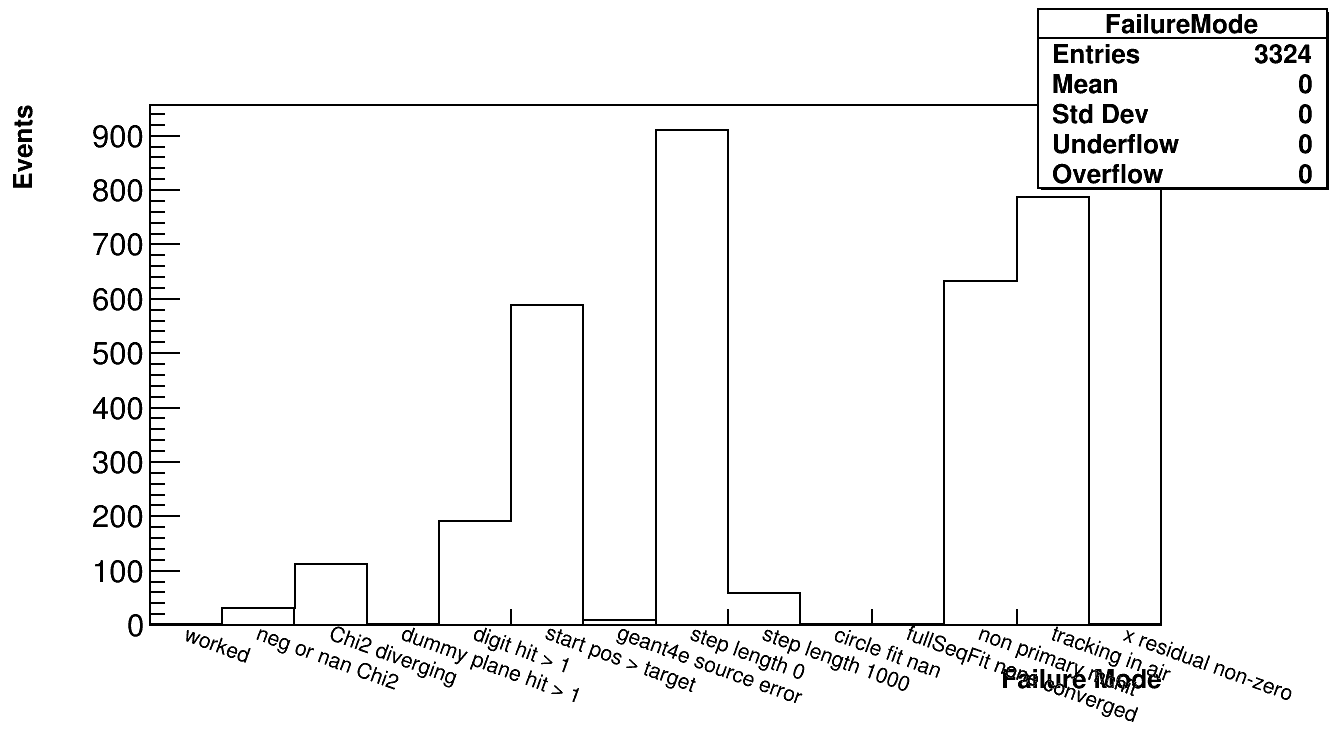
\includegraphics[width=1.0\textwidth]{FailureModesExample}
          \label{fig:failureModes}
        \end{figure}

      \item{\bf{GeanePoorEvent\_module.cc}} \\
      A filter to separate out poor tracks, defined as having a pull value (in any of the 5 parameters on plane 0) of greater than 5 (or less than -5). If the track fitting is working correctly, then the pull distribution lies between -5 and 5 (occasionaly a single event can be just outside that range). For more reaslistic data however, particles will lose energy after interaction with material, which the track fitting doesn't perfectly account for (since it handles averages), and these events can be designated as ``poor'' though they are real. The more important tracks are the ones which have no energy loss but are still ``poor'' - these tracks are bugged in some way.

      \item{\bf{geanePlotsMacro.C}} \\
      A little macro I wrote to combine various plots produced with the GeanePlots analyzer. Useful for looking at things like pull distributions as a function of plane or track length.

      \item{\bf{haddGEANE.sh}} \\
      This isn't an analyzer, but I figured I'd put a note here on this script which is hadds (Root macro) the output files from the GeanePlots analyzer. It is currently deprecated, having been hardcoded to hadd 1000 files (skipping missing files) with delineaters {NAME}{0..999}, where the latest updates to the grid and produced file names don't necessarily follow this pattern. However it might be useful to revive this file at some point in the future.

    \end{enumerate}


  \subsection{Other useful fcl files}

    There is a number of other fcl files which are currently included in gm2tracker which are useful for various analysis or fitting purposes. These are relatively simple and straight forward fcl files which can be deleted, combined, or changed however the user wishes depending on what they are looking at. They are typically used on produced sets of GEANEArtRecords.

    \begin{enumerate}

      \item{\bf{RunGeane-midasdata.fcl}} \\
      A simplified fcl file for performing the Geane fitting reconstruction on actual or fake midas data, with fcl parameters set or removed accordingly.

      \item{\bf{RefitGeane.fcl}} \\
      This file simply refits a previously produced set of track candidates, typically used for refitting failed or bad events from a previous attempt at fitting. One can make changes to the fitting code, refit, and compare to previous results.

      \item{\bf{makeGEANEPlots.fcl}} \\
      This file will call the main GeanePlots analyzer module for producing plots about the GEANEArtRecords, useful for making plots after tracks have already been produced. (Plots may be added or removed as well.) Note that with the grid updates, it's now necessary to perform the reconstruction and analyzer stages separately, so this fcl file is convenient in that it only includes the latter.

      \item{\bf{ProcessSelectionGeane.fcl}} \\
      This file will call the filter on different physical processes that events have undergone within the tracker region (ionization, multiple scattering, bremsstrahlung), if one wishes to separate events based on this criteria. (Note that the module that this fcl file calls is not fully finished, nor is it so clear how this filter should work exactly.)

      \item{\bf{makeGeaneSingleEvent.fcl}} \\
      This file will take produced GEANEArtRecords and call the single event analyzer on the passed in file(s) or a specified set of events. This is useful for analyzing single events to see where rare errors crop up, if tracks are kinking, for debugging purposes, etc. This should not be used for a large number of events.

      \item{\bf{filterTracks.fcl}} \\
      This file will filter on whether art events successfully produced a GEANEArtRecord or not (succeeded or failed) through the TrackFilter\_module.cc, which is useful for reducing the size of art files which contain many events that do not hit the tracker or don't hit enough planes. There is also an option to filter on StrawArtRecords directly before attempting to fit.

      \item{\bf{fileMerge.fcl}} \\
      This file will simply combine the set of art files that are passed to it, useful for reducing the number of files one has to deal with.

    \end{enumerate}



\section{gm2Geane package in artg4 - eloss, brems, ionizations, msc}
\label{sec:gm2Geane}

See many docdbs by Nick Kinnaird on geane updates for more info if wanted. Summary of stuff here.


  There is a folder under artg4/gm2Geane, where slightly (but importantly) modified geant/geane code that the geane track fitting uses is located. Most importantly is that the reconstruction was taking too much energy away from the particle during propagation due to bremsstrahlung, so that has been removed. (Thanks James for help with this.) (Probably explain flow of file - extrapolator tables etc.).

  Besides those associated files, all files from the geant folder ``error\_propagation'' have been copied into this directory as well, with the only non-name changes lying in gm2GeaneFreeTrajState.cc. (Many files had to be copied due to naming/linking - some could probably have been omitted but I decided to copy the whole folder.) Ionization and multiple scattering errors have been modified according to Lavezzi thesis (explain more) - with no improvement in results unfortunately. (Probably turn defaults back to original code (still gm2Geane) with the option to turn things on somehow if desired - at least leave them in for future tuning.)

  \cite{Lavezzi}

Should I go more in depth about the error\_propagation/gm2Geane source code? Probably - at least for certain main files.

% it seems I have to cite the references in order for them to be added to the paper - some weird build issue, just do it here until I cite them naturally in the paper
\cite{energyloss}

\begin{figure}[]
\caption{Shown here is the energy loss between the first and last hit in the tracker from simulation. (Momentum magnitude difference.) Sources of energy loss come from ionization and bremsstrahlung processes, which account for the long Landau tail running off to infinity. The distribution has a mean of approximately 220 keV and and peak centered at about 150 keV, which is reasonable for the material composition of our trackers and tracker gas. More than 50\% of the energy loss comes from the mylar walls of the straws as seen in the simulation.}
\centering
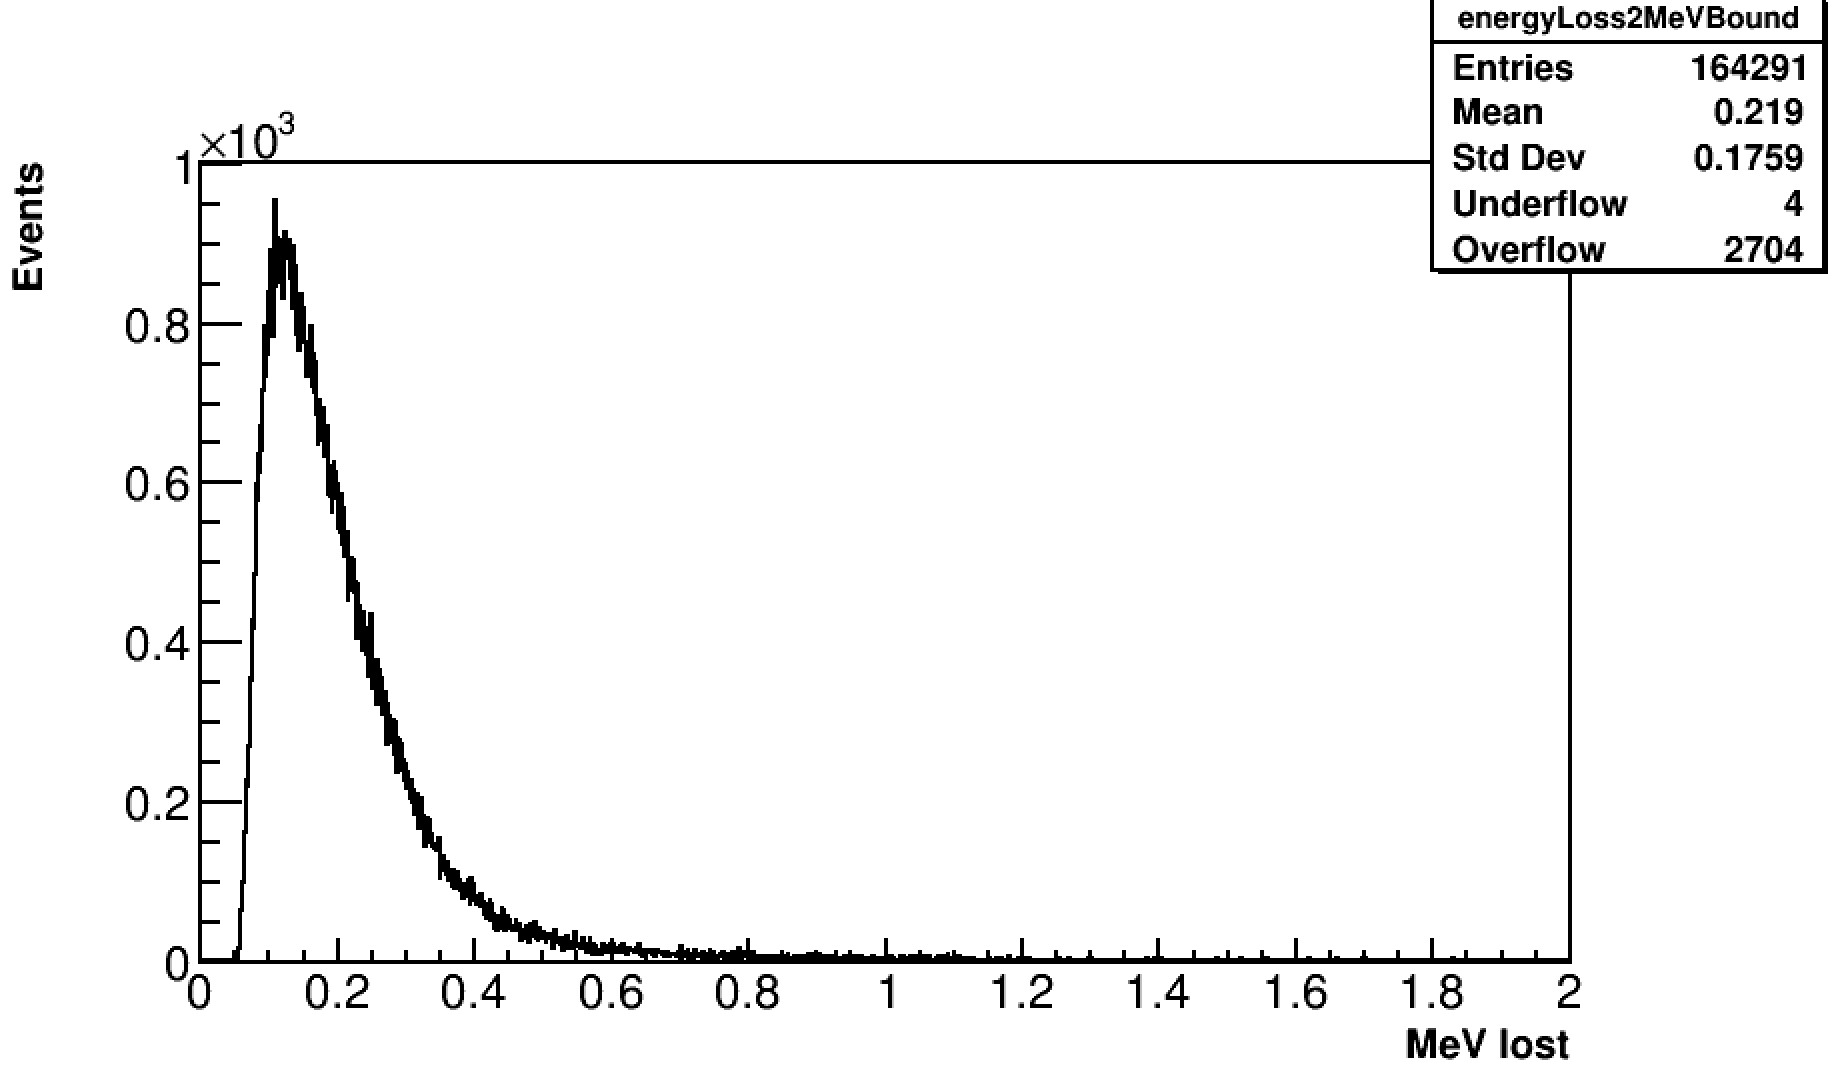
\includegraphics[width=1.0\textwidth]{eLoss}
\label{fig:eLoss}
\end{figure}

\begin{figure}[]
\caption{It was noticed during the course of debugging that the Geant4 error\_propagation routines were consistently removing too much energy on average from all tracks as they passed through the tracker during reconstruction. It was discovered that the Geant4 tables were taking out too much energy due to bremsstrahlung processes and it was decided to remove this effect. The left plot shows in a red the true particle momentum as a function of X distance through the tracker, and in black the reconstructed momentum before bremsstrahlung was taken out of the reconstruction for a single event. The differing slopes signify the problem. The right plot shows the same event but with bremsstrahlung taken out. Notice scale change, and that the reconstructed momentum aligns much more readily with the truth.}
\centering
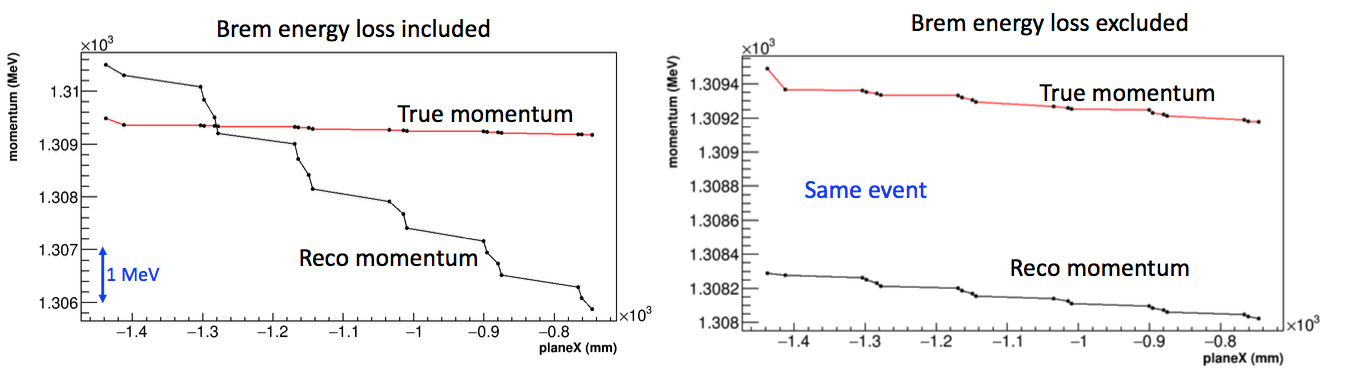
\includegraphics[width=1.0\textwidth]{bremComparison}
\label{fig:bremComparison}
\end{figure}


\section{Left-Right}
\label{sec:LR}

	This section will describe the fitting modes that can handle determining the left-right sides of the hits within the fitting. The first and shorter section describes the ``mainFit'' fit mode and the second and longer section describes the ``fullSeqFit'' fit mode. Some of this information is repeated from the GeaneFittingUtils.cc section describing these fit modes. It is important to remember that while some left-right information for the track may be determined upstream, most of it cannot until a fit of some sort is completed. For us that is the wire fit, which does not require any left-right information in order to work. The wire fit serves as the starting point for determing the left-right sides of the hits since the overall fit will approximately get the left-right sides correct, though not always. Even a single hit side being incorrect can throw the fit off, which is usually readily apparent with resulting high $\chi^{2}$s or low p-values. Sometimes this incorrect side (or sides) can be determined by looking at the individual plane $\chi^{2}$s and finding the outliers, though this is not always the case. Due to the smearing of the real dcas from the straw resolution, sometimes it can be very difficult to determine the left-right sides in all hits. There is planned to be a refinement stage in the future, which will be tasked with adjusting the track that is to be fitted, both dealing with left-right sides and removing or adding hits to the fit. Until such a time however, we are unable to fit all tracks correctly with 100\% fidelity due to this left-right ambiguity problem.

	\subsection{mainFit}

	  First a wire fit is completed with a couple of iterations. Then a fit is performed where each iteration takes as it's hit sides wherever the previous fit ended up. Something like 2/3rds of the tracks converge nicely with this method, but not all. (In the current iteration of the code there is also an intermediate second wire fit, where the known sides from the doublet geometry and track angle are set, which helps salvage a couple of tracks.) If the left-right sides are only taken from the wire fit a single time, instead of being updated each iteration, then less tracks converge.

	\subsection{fullSeqFit}

      This fitting mode takes the longest time to fit a track, because it checks every single LR combination for all hits in order to find the best track. It starts by first doing a wire fit for all hit digits in order to get approximate track objects (transport matrices, error matrices, predicted parameters) used for making approximate guesses at how good different LR combinations are. Second, one can lock certain hits to left, right, or center depending on how the user is fitting (locking LR from known geometry, small dcas, etc), and the track fitting will loop over the remaining unknown sides, checking each combination. In order to increase the speed of this code greatly, instead of checking all $2^{N}$ combinations directly, the separate $2^{Nu}$ and $2^{Nv}$ combinations are checked separately (leaving the other parameter sides as being set to the wires). See Figure \ref{fig:SeqCheckSteps} for a diagramatic view of exactly how this approximate fitter works for the sequence checking, and read the \hyperref[sec:GeaneLRUtils]{GeaneLRUtils.cc} section for detail on the methods that are used within the fullSeqFit.

			\begin{figure}[]
				\caption{This figure shows the steps used to determine an approximate set of the best U and V left-right sequences. Note that these steps are followed separately but identically for U and V. The equations here are identical to some of those given in the \hyperref[sec:Formalism]{Formalism} section. Step 1 is performing a wire fit, done once for all $2^{N}$ U or V combinations. The resulting generated transport, error, and covariance matrices along with the predicted parameters from the wire fit are saved for the following steps. Step 2 involves using those aforementioned matrix objects, but now with the measured positions in the calculation replaced with whatever particular left-right sequence we're checking. An approximate fix to the track is then calculated, which can be used in step 3 to determine a new set of approximate predicted parameters. These approximate predicted parameters are then combined with the measured left-right sequence we're checking in step 4, along with a hybrid error matrix (where if we're checking U sequences, then the V planes have wire errors, and vice versa) to calculate an approximate $\chi^{2}$ for that particular sequence. All U and V sequences are checked and the best 10, with the lowest $\chi^{2}$s, of each are saved. The arrows show where matrix objects are used from one step to another. This method while still slow for many combinations, especially high N tracks, is pretty fast because it's simple matrix multiplication over and over again, without actually Geane fitting eaching $2^{N}$ combination. (And no inversions.) Note that while not as effective, it is possible to jump from step 1 to step 4, where the predicted parameters remain as those predicted from the wire fit, and calculate an approximate $\chi^{2}$ for the left-right sequence. This has the benefit of being faster by skipping steps 2 and 3 but fails for more events, and so isn't as useful.}
				\centering
				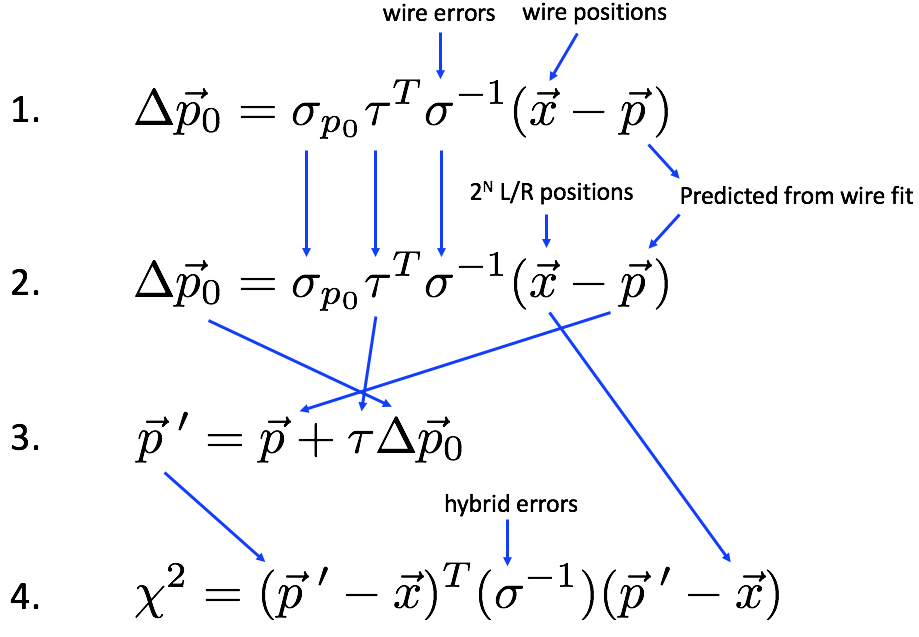
\includegraphics[width=0.8\textwidth]{SeqCheckSteps}
				\label{fig:SeqCheckSteps}
			\end{figure}

 	  Once the set of best U and V sequences have been determined with the approximate fitter, they are combined together and fitted with the full Geane error propagation fitting. For a small sample of fitted tracks, Figure \ref{fig:PositionOfBest} shows where in the set of best 10 saved $\chi^{2}$s for the different sequences the actual truth sequence is. (For a larger sample of tracks, this plot would fill out more with less empty bins.) It can be seen that the approximate fitter actually guesses the correct U and V sequences a large percentage of the time. When combining the U and V sequences together and full fitting, it is beneficial to scan over some smaller set instead of the full 10 by 10 grid. The red line in the figure separates out a set of 15 tracks to full fit, which results in high fidelity of fitted tracks. If one wishes an even smaller set of tracks can be full fitted, where more tracks will result in poor fits, but the speed of the tracking improves significantly. See \href{https://gm2-docdb.fnal.gov/cgi-bin/private/ShowDocument?docid=6800}{DocDB 6800} for a quick study of track fitting speed vs the level of results, where one should pay attention to the number of tracks within the 0 bin, representing poorly fit tracks coming from incorrectly chosen left-right sequences. 

 	  It is also possible to cut short the sequences that are being full fitted. When there is a couple of very similar sequences, possibly with small dcas, the track fitting results in similar $\chi^{2}$s. Usually soon after there is a large jump in the full fitted track $\chi^{2}$ as some left-right choices have been changed, revealing that that particular sequence and the ones after are incorrect. For example the $\chi^{2}$s might go as 10.2, 11.4, 10.3, 38.9..., and it is at this large jump that one can make a reasonable assumption that the best sequence has been found. This of course does not work perfectly all of the time but it is a good way of eking some more speed out of the tracking. The user can configure the fitting (from base fcl parameters to options such as describe here) to optimize vs fit results or speed however desired. This should be combined and studied with the future refinement stage. One might wish to do faster fits to start and refine the poorly fitted tracks before doing more thorough sequence checking and the like.

			\begin{figure}[]
				\caption{The fullSeqFit mode saves the smallest 10 $\chi^{2}$s from the approximate fitter for the ``best'' U and V sequences. For the set of 10 best U sequences, the X bins in this plot represent the location of the true U sequences, and similarly for V. For example, if the 0 bin is filled then the U sequence with the smallest $\chi^{2}$ is the true sequence, if the 1 bin is filled then the U sequence with the second smallest $\chi^{2}$ is the true sequence, etc. It can be seen that the approximate fitter does a very good job of actually guessing the true U and V sequences with the bottom 3 bins holding most of the events. Some sequences do end up in the higher bins where the approximate fitter has not done so good of a job at determing the true left-right sequences, including some events which end up in the overflow bins where the approximate fitter has simply failed. The angled red line describes a region of combined sequences to perform the full fitting over in order to try and find the combined true left-right sequence. Note that even then the true sequence may not have the smallest $\chi^{2}$ in the final fitting due to the smearing of dcas. Note also that hit digits with very small dcas will have very similar $\chi^{2}$s and fill neighboring bins, though this fact is ignored when locking small dcas to the wire centers.}
				\centering
				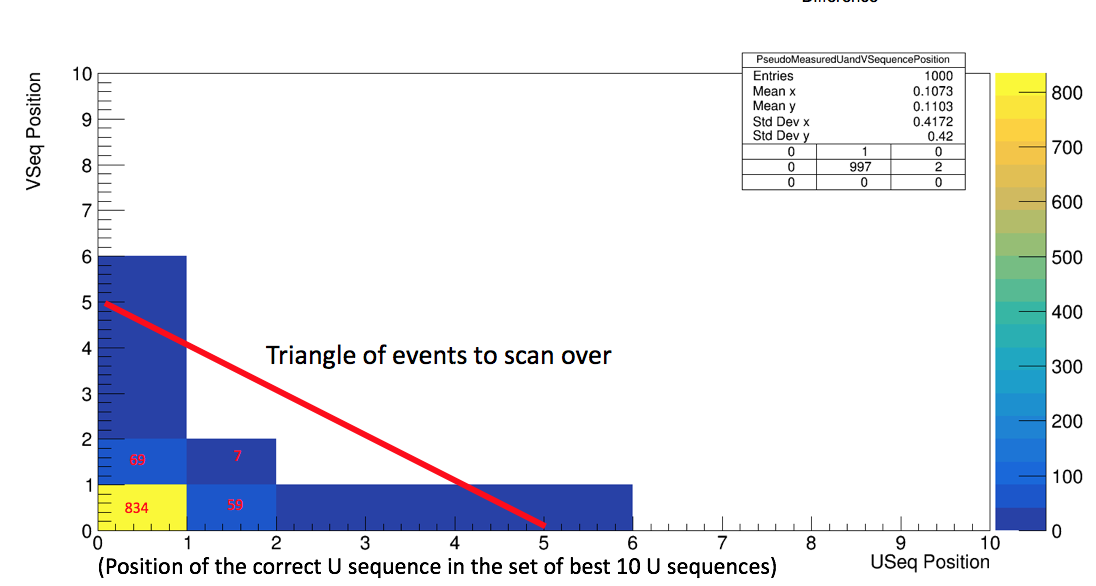
\includegraphics[width=1.0\textwidth]{PositionOfBest}
				\label{fig:PositionOfBest}
			\end{figure}

% \begin{align} %\label{eq:corr}

% \Delta \vec{p}_{0} = \sigma_{p_{0}} \tau^{T}\sigma^{-1}(\vec{x}-\vec{p} \hspace{.05cm} )
    
% \vec{p} \hspace{.1cm} ' = \vec{p} + \tau \Delta \vec{p}_{0} 

% \chi^2 = (\vec{p} \hspace{.1cm} ' -\vec{x})^{T} (\sigma^{-1}) (\vec{p} \hspace{.1cm} ' -\vec{x})

% \end{align}


\section{Coordinate Systems}
\label{sec:Coord}

  The only material not covered here in full detail is the mathematical explanation of reference frames, for which one should see the reference papers. It suffices to summarize as follows: GEANE objects (matrices and parameter vectors) are defined and calculated in the Geant4 source code in the free particle system. Then there is an intermediate surface system defined in XYZ, as the Geant4 surface trajectory system must be defined in an orthogonal coordinate system, before which parameter objects are converted to the most natural detector system of XUV. (Important note - be very careful with coordinate system variables, letters are reused between different papers and code bases with different configurations and meanings constantly.)


Notes on coordinate systems I use - UV pointing outward vs XYZ, XUV x being forward, UVW in geante src, maybe IJK/TUV in one paper-prob not, GeaneTrackerWorld[0,12,18], rotateArcTracker (bit more specific), magnetic field access coordinates?, JacobianToUV
- this should be in coord sys file



\begin{figure}[]
\caption{Shown here is a picture of the 3 trackers in the world geometry in their approximate positions. First note the world coordinate system shown in the bottom left of the plot, where the origin lives at the center of the ring. Tracks are then generated and read out from the trackers in their three world positions in red. Due to the reconstruction bug where tracks improperly reconstruct if their momenta is too aligned with the globabl Z axis, the reconstruction rotates the entire arc including tracker 0 to the blue position, where planes are parallel in X, and this problem is avoided. Track parameters from the 3 positions are then rotated to this reference frame by the amounts shown on the plots for the reconstruction stage, and at the end are rotated back.}
\centering
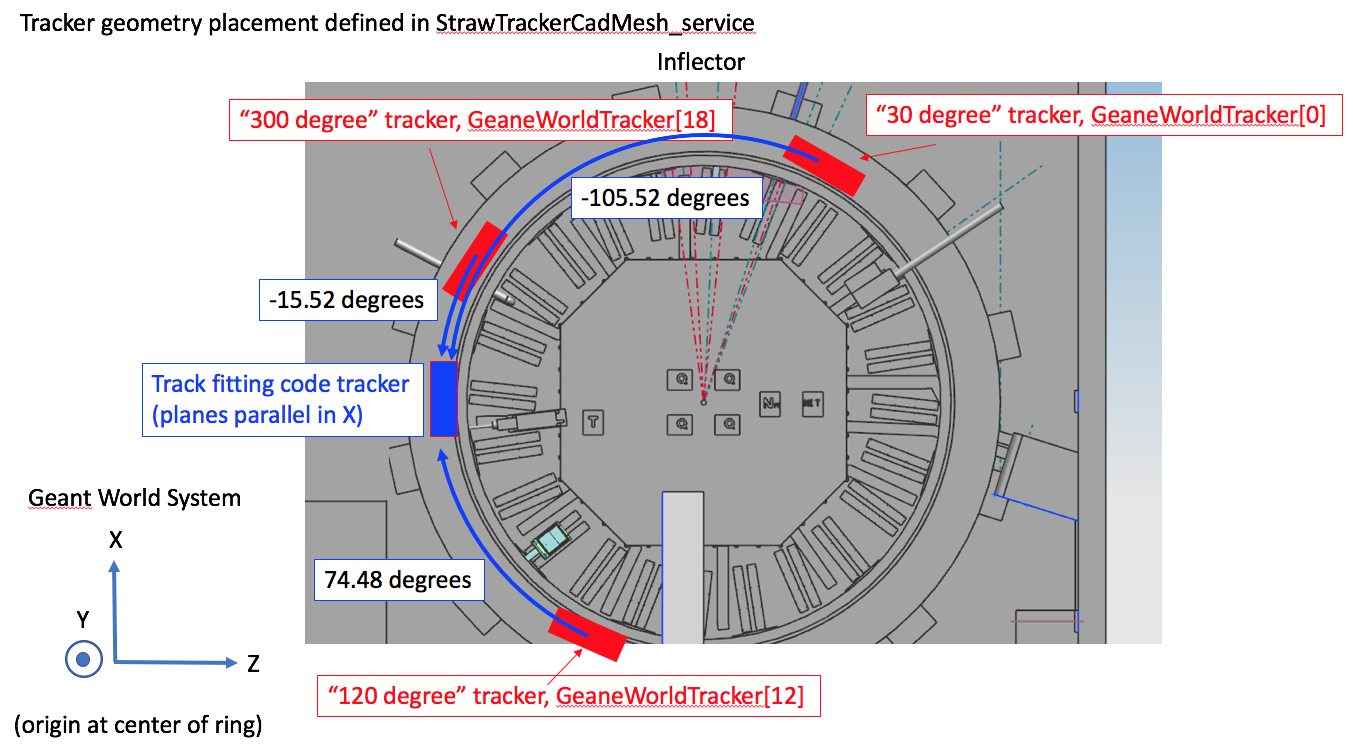
\includegraphics[width=1.0\textwidth]{WorldCoordSys}
\label{fig:WorldCoordSys}
\end{figure}

\begin{figure}[]
\caption{This picture shows the coordinate system in which the the Geane track reconstruction is performed, in relation to the world coordinate system. The origin remains at the center of the ring, with the tracking planes parallel in X in the reconstruction, going forward in number. Y is vertically up, and Z is horizontally to the right. U and V are defined such that they have greater values with higher radii and increasing straw number.}
\centering
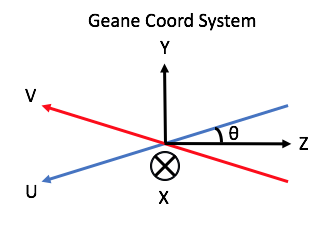
\includegraphics[width=0.6\textwidth]{GeaneCoordSys}
\label{fig:GeaneCoordSys}
\end{figure}


$1/p, \lambda, \phi, y_{\perp}, z_{\perp}$, free system

$1/p, py/px, pz/px, y, z$, surface system

$
\begin{pmatrix}
u \\
v \\
\end{pmatrix} =
\begin{pmatrix}
-\sin{\theta} & -\cos{\theta} \\
\sin{\theta} & -\cos{\theta} \\
\end{pmatrix}
\begin{pmatrix}
y \\
z \\
\end{pmatrix}
$, yz to uv matrix, where $\theta$ is $7.5\degree$, the 5x5 transformation is just a 1 in the top left corner, and then this matrix in the remaining 2 diagonal blocks

$1/p, pu/px, pv/px, u, v$, uv system




Secondly, the RunGeane.fcl file loads all 3 trackers necessary for symbol and name definitions, but such that tracker 0 (or 18) is rotated such that the tracking planes are parallel to the global geant X axis (using the rotateArcTracker fcl parameter for the Arc service). This is done to avoid the issue of error propagation instability close to the Z axis, as detailed in \href{http://gm2-docdb.fnal.gov:8080/cgi-bin/ShowDocument?docid=4567}{DocDB 4567}, while at the same time still observing the correct azimuthally symmetric 2D field for the tracks.


\section{notes and other}

  \subsection{Initial Errors}

  When perfoming the Geane fitting and error propagation as described in the \hyperref[sec:GeaneParamUtils]{GeaneParamUtils} section, the error matrix from material is generated and grows as the tracked particle passes through more and more material. This error matrix can however be intialized with some values other than 0. It seems like it might make some sense and improve the fitting if this trajectory error was filled with values representing the error in the intial circle fit to the wire centers which serves as the first guess at track parameters. However perfect pull and p-value distributions were obtained in the vacuum case (and close to in the material case) without these errors, leading me to believe that they are not necessary. I'm including this note here to bring attention to future developers of this unclear fact.



  note on older branches for development at all?



  \subsection{Kalman Filter}

    There is some precedent for using the error propagation matrix objects within a Kalman filter as detailed in the Lavezzi thesis \cite{Lavezzi}, but due to the circumstances following the creation of this code that technique was not followed. At the beginning of development, a Kalman filter was being started in tandem by others, which has since fallen by the wayside. One of reasons for choosing the least squares global minimization was in order to have two separate methods for fitting. The simpler method was also chosen as I was unfamiliar with track fitting and coding in general when beginning development. (The primary reason was the introduction by Rob Carey, who worked on the traceback in the E821 experiment.)






Where to structure this in the file?

Notes on coordinate systems I use - UV pointing outward vs XYZ, XUV x being forward, UVW in geante src, maybe IJK/TUV in one paper-prob not, GeaneTrackerWorld[0,12,18], rotateArcTracker (bit more specific), magnetic field access coordinates?, JacobianToUV
- this should be in coord sys file

accessing the field in a specific way



\section{Future To Do}

	There is always more to do when it comes to tracking. Improvements to the fitting code, optimization, integration of new features up and down stream, and general code development are a few areas that will require work in the future months and years that this code is in use. Listed here are a few specific sections of work that need to be done, though it is not all inclusive. Some of these sections are hinted at in other parts of this document, some of them are included here as possible sections of work (though not necessarily), and some sections are for work that was started but not completed. These are not ordered in any particular way. (These also might have been taken care of by the time the reader looks through this document.)

	\subsection{Non-Gaussian Garfield Errors}

		When dealing with real data, the errors on the dca measurements that the straws record are non-Gaussian, stemming from the fact that the drift model is non-linear. To align as best we can with real data, James Mott has developed a Garfield model to deal with these measurement attributes, see \href{https://gm2-docdb.fnal.gov/cgi-bin/private/ShowDocument?docid=6171}{DocDB 6171}. However, this still causes trouble for our least squares minimizer since it assumes that the fit errors are Gaussian. If one implements the Garfield model directly in the simulation, then the resultant p-value plot rises at both 0 and 1, see Figure \ref{fig:garfieldPValue}. For this reason these fit errors and their affect on the track fitting need to be studied, understood, and improved where possible, though it is reasonable that their affects are unavoidable.

			\begin{figure}[]
				\caption{Shown here is the p-value distribution for fitted tracks using the Garfield parameterization for the dca errors. It can be seen to spike at 0 and rise towards 1, when in an ideal case it would be uniform, indicating that the fitting is not handling the errors exactly correctly. This is probably unavoidable on some level, but can probably be improved from where it's at now.}
				\centering
				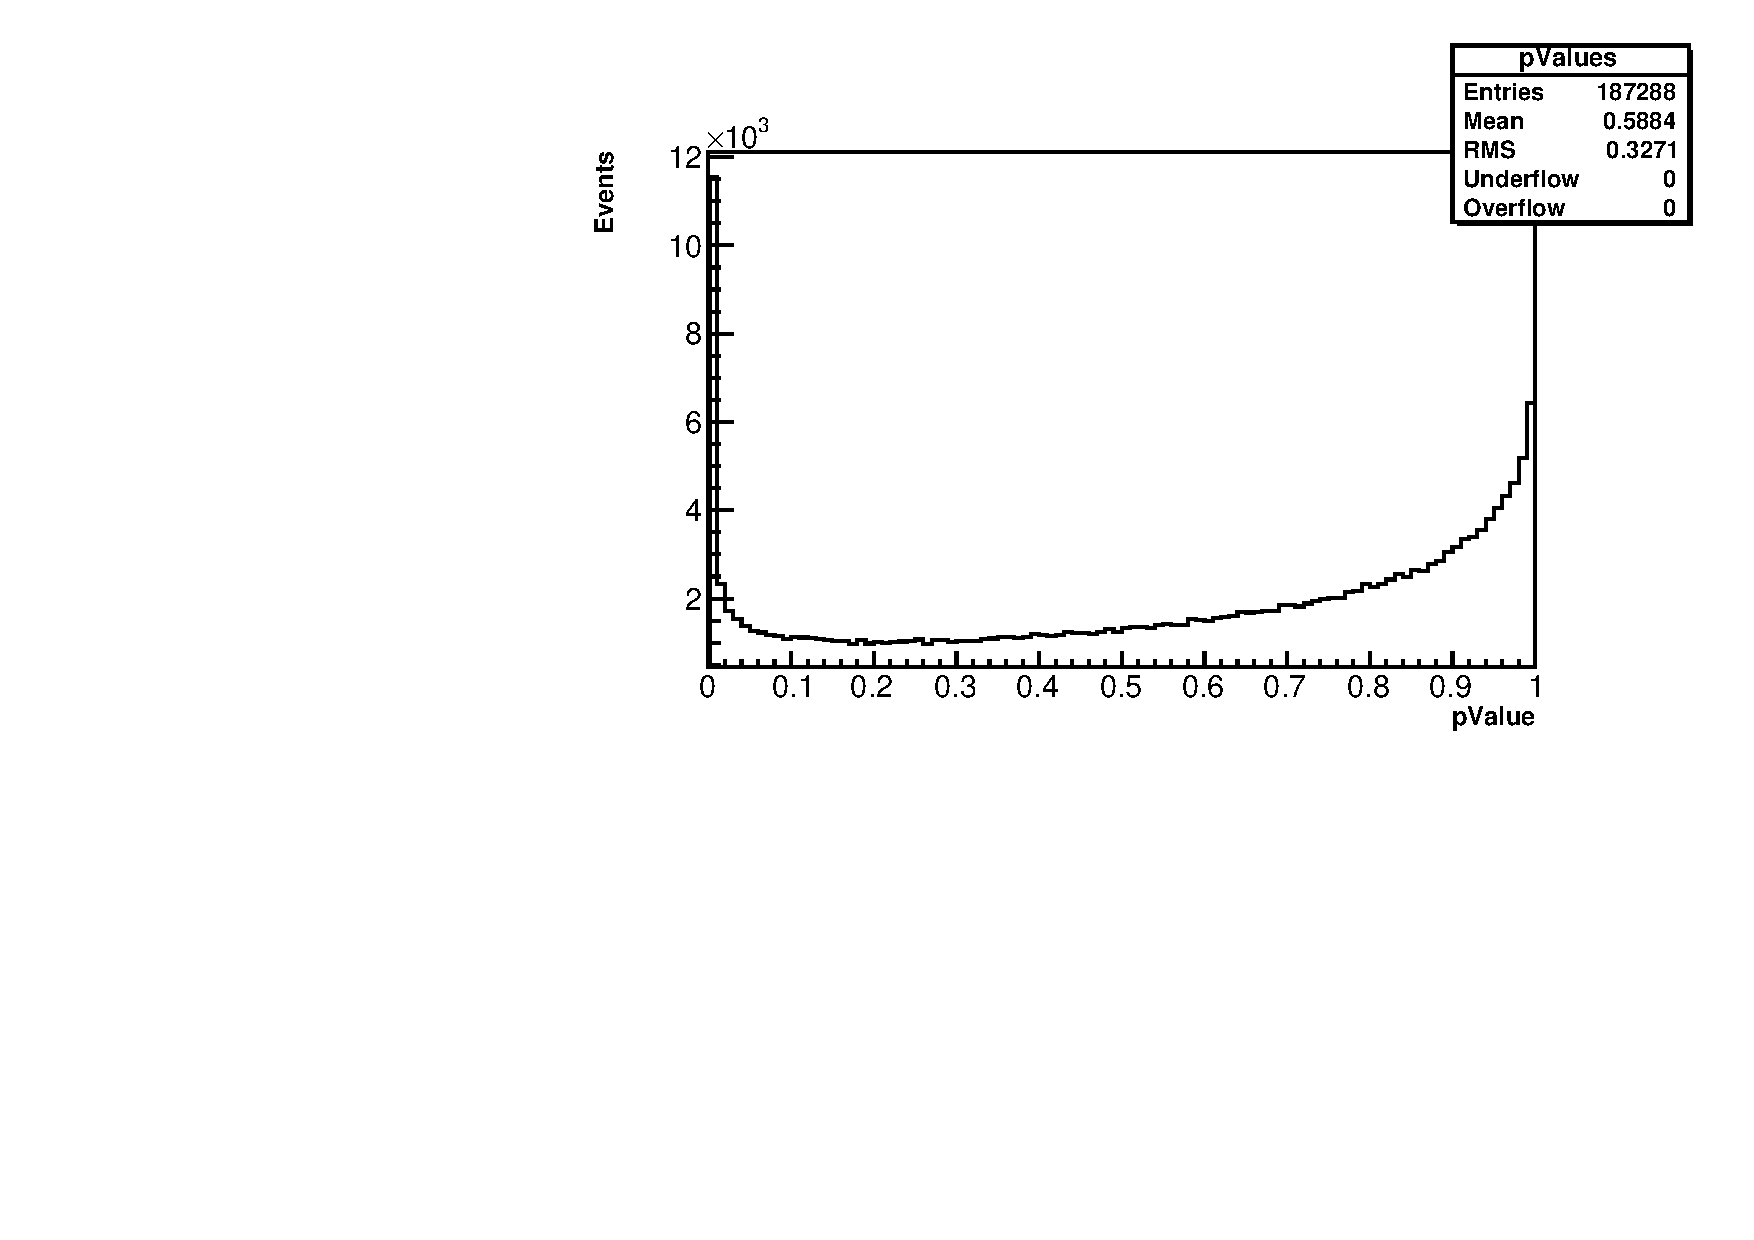
\includegraphics[width=1.0\textwidth]{garfieldPValue}
				\label{fig:garfieldPValue}
			\end{figure}

	\subsection{Measurement pulls on all planes}

		Currently in the track fitting, the measures of how well the track fitting is performing is to look at truth pulls for the parameters on the starting plane as well as the p-value distribution of the fitted tracks. Unit Gaussians for the former and a uniform distribution for the latter prove that the track fitting is working properly. With real data however, the former do not exist, and it is instead more instructive to look at measurement pulls on hit planes. Section 6 of reference \cite{trajfit} has some information on this, with the mathematical form of these measurement pulls defined as:
		\begin{align} \label{eq:measpull}
            \frac{\Delta_{meas}}{\sigma} = \frac{p_{fit} - p_{meas}}{\sqrt{\sigma^{2}_{meas} - \sigma^{2}_{fit}}},
        \end{align}
        where all terms are defined on a single plane.

        However, if these measurement pulls are implemented as in Equation \ref{eq:measpull}, then the resulting distributions are not unit Gaussians as they should be. If I define them as 
        \begin{align} \label{eq:measpullmaterial}
            \frac{\Delta_{meas}}{\sigma} = \frac{p_{fit} - p_{meas}}{\sqrt{\sigma^{2}_{meas} - \sigma^{2}_{fit} + \sigma^{2}_{material}}},
        \end{align}
        where $\sigma_{material}$ is the error due to the material only, then the resulting distributions look more correct. See \href{https://gm2-docdb.fnal.gov/cgi-bin/private/ShowDocument?docid=6261}{DocDB 6261} and \href{https://gm2-docdb.fnal.gov/cgi-bin/private/ShowDocument?docid=6306}{DocDB 6306} for calculations and plots regarding this. The problem however is that this doesn't seem to make a whole lot of conceptual sense, adding this extra error term in. Either this extra term is supposed to be added for reasons not fully understood, or it counteracts some mistake in the measurement pull calculation. Understanding and utilizing this will be necessary when it comes to looking at real data.

	\subsection{Material error tuning}

		While less serious than dealing with the non-Gaussian measurement errors as described above, it will almost certainly be necessary to deal with the material errors as calculated in the Geant4 error propagation routines, specifically the methods ``PropagateErrorMSC'' and ``PropagateErrorIoni'' in the gm2GeaneFreeTrajState.cc file which calculates these material errors. See the \hyperref[sec:gm2Geane]{gm2Geane} section for some more details on this. The reference \cite{Lavezzi} has some sections on the calculation of these errors for the PANDA experiment, and it is readily observed that these calculations differ slightly from those implemented within Geant. This is supposedly because the default Geant calculations are more attuned to denser scatterers, and not PANDA's straw tube tracker which has some resemblance to our straw detectors. This suggests that we should also be making changes. These modifications are currently programmed into that gm2GeaneFreeTrajState.cc file but commented out. Some quick studies with them turned on were done but no real conclusions were made about whether they should be included in our error calculations or not. It is decently likely that some modifications will need to be included in the error calculations, but that they will not be exactly equal to the ones that PANDA used. It is certainly the case that the p-value distribution right now does indeed rise very slightly towards 1, hinting at not-quite-correct error calculation. The measurement pulls can also be a window into the correctness of these error calculations, but first those pulls need to be understood as described above before they are useful.

	\subsection{Starting error/covariance}

		When first creating the free trajectory state for the error propagation, you need to initialize the 5x5 error matrix. For our tracking we've just been using a 0 matrix. That's given us ideal results in a vacuum world, and near ideal results in a material world (with known effects throwing distributions slightly off), indicating that we're performing the track fitting correctly. However it seems like it would make conceptual sense to calculate some error on the track parameters from the initial fitter and use that as an input, as there is an uncertainty in where the track can go that you would want to include.  In the same vein, it seems like it would make sense to use the previous fit iteration covariance matrix as the input error matrix for the next iteration. If any of this is included then the fitting results always worsen however, so they have not been included. This work might be unessecary, but I've included this note just in case.

	\subsection{Initial fitter and effects on Geane fitting}

		For the track fitting, an initial guess for the starting track parameters is needed before doing the Geane fitting. Currently a simple horizontal circle fit to the wire centers is performed upstream in the track finding code. This circle fitter does a remarkably sufficient job for the vast majority of tracks. There are some tracks which do not converge however, and it is possible that this is because the initial fitter is insufficient. That and the fact that the intial fitter was done simply without much thought means that it might be a good place to eek out some better tracking results. General studies on how good this initial fitter needs to be have yet to be completed also, though it's reasonably likely that it's already sufficient. It is also the case that while no biases due to this have been observed with simulated data, they might rear their heads with real data which is something to keep in mind.

	\subsection{Bugs and failed tracks}

		There are always tracks which fail the tracking for one reason or another. See Figure \ref{fig:failureModes}. Some of these are due to unavoidable effects like kinking after interacting with material, and some of these are from very fixable sources. Any tracks which fail due to bugs in the tracking code should absolutely be fixed. Known failures included Geant bugs where the step length is 0 or 1000 mm, a 0 transport matrix is returned in the error propagation stage, the error propagation has gotten past the target, or the error propagation returns an internal failure. The exact sources of these bugs are difficult to determine considering that its Geant source code where the problems lie. Some tracks also begin error propagation within the material G4\_AIR, and those have been marked to fail. This might be occuring because the intial fitter does so poor of a job that the track starts outside the storage region, or something more sinister might be going on. There is also a bug where in a vacuum world some tracks experience physical processes like ionization or bremmstrahlung (\href{https://gm2-docdb.fnal.gov/cgi-bin/private/ShowDocument?docid=6183}{DocDB 6183}), which causes some simulated tracks to reconstruct poorly (though not necessarily fail directly). James Stapelton will at some point look more into this since it has some deeper Geant source, but it's good to keep in mind.

		There are still some tracks however that return negative or nan $\chi^{2}$s which have unknown sources. These combined with tracks that diverge leaves a set of tracks that while small are the most important to really understand and fix wherever possible. The latter can probably be improved with a better initial fitter though not fully removed. (There are also some tracks which don't diverge, but also don't converge with a very small $\Delta\chi^{2}$ between iterations, though these are technically not designated as failures.) Finally there are sources of failures from the upstream tracking code. While most such problems have been fixed, there remains the tracks which end up with more than one digit on a single layer, which the Geane fitting cannot handle. It is also very likely that more unseen issues exist since this is a very complicated chain of track reconstruction.

		With further development of the tracking code, both locally, in the upstream reconstruction chain, or even the greater surrounding framework, more bugs or failed tracks will arise. Such new bugs will usually manifest themselves in tracks with negative or nan $\chi^{2}$s, so if the number of such tracks increases then once can be reasonably sure that a new problem has arisen. This is natural and unavoidable, and it is simply a matter of fixing these issues as they appear. Similarly, as data comes in there is a good chance that new failures will appear, which could possibly be due to more subtle issues. (Though I should mention that no such things were seen with the wire fits on the commissioning data.)

	\subsection{Physical processes and kinked tracks}

		As detailed in the \hyperref[sec:AnaFilt]{Analyzers and Filters} section, there is some code that has been partially written regarding the physical processes that the simulated tracks undergo. It would be a good idea to really undertand the effects on the track fitting due to these physical processes. There is a little bit of information on this in \href{https://gm2-docdb.fnal.gov/cgi-bin/private/ShowDocument?docid=6099}{DocDB 6099}. It is certainly the case that because the Geane fitting creates average trajectory states and adds the error due to material, most tracks are properly treated, but there are some tracks which kink or lose a larger amount of energy and fit poorly. These can usually (but not always) be removed from the tracking results with an energy cut for simulated events. For real data however these effects will still exist. Understanding them and reducing them until they are irreducible will be a necessary step before really looking at all the tracks from data. Certainly for kinked tracks, it should be possible to identify them with some smarter criteria in the analyzer stage other than just looking at event displays as in Figure \ref{fig:Kink}. There is some unfinished code (with some sort of unknown issues) in the GeanePlots module which looks at the TrajectoryArtRecords for this reason, which has been left in for the future.

			\begin{figure}[]
				\caption{Shown here is a position plot from the GeaneSingleEventViewer analyzer. The black dots on the red line indicate the true positions of the track that is being reconstructed, with the red line simply connecting the dots. The black line and dots indicates the reconstructed track and positions. The view is side on, with the X axis being the X position of the hits in the reconstruction frame, with particle direction going from left to right as particles pass through the different straw layers. The Y axis indicates the Y position of the track. It can be seen that the true track has upward momentum at the start, hits some material, and kinks at about -1440 mm. (It starts curving back upwards further on because this track was located in a region with some radial field component.) The Geane fitting does it's best to form an average reconstructed track which is seen to be a smooth approximation to the kinked track. This will of course result in a fit with a large $\chi^{2}$.}
				\centering
				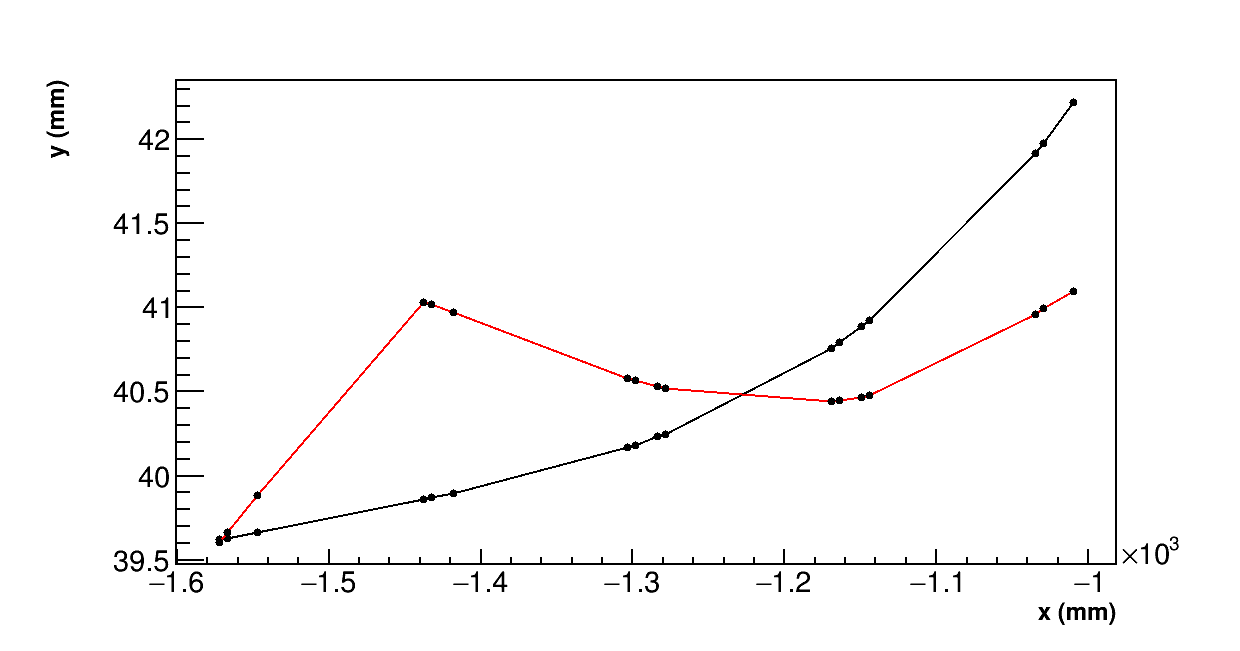
\includegraphics[width=1.0\textwidth]{Kink}
				\label{fig:Kink}
			\end{figure}

	\subsection{Tracker alignment geometry and magnetic fields}

		Currently in the simulation and reconstruction all trackers have the same perfect placed geometry with wire planes exactly parallel to one another. In reality the different trackers will have slightly different geometry due to imperfect placement into the vacuum chambers as well as slight wire warping. See Figure \ref{fig:Alignment}. Once the alignment is completed as best it can be, both physically improved and misalignments recorded (Gleb Lukicov and others), the resultant geometry differences should be coded up and included for the best results possible. It's not clear to me exactly what this will entail, or what complications in the fitting will arise but it should be kept in mind. Certainly the track fitting results without this are worse since the Geane fitting assumes parallel measurement planes, which is not quite the case.

			\begin{figure}[]
				\caption{Shown here is a toy model of the alignment code being developed by Gleb Lukicov. The circles represent the straws with the shaded circles being the hits. In the upper picture an exaggerated vertical misalignment in the two center modules can be seen, with the lower picture being the ideal geometry. In red are the straight line fitted tracks to the hit straws. It can be seen that the misalignment in the top picture produces tracks which differ from the true tracks in the lower picture. This means that without the alignment included in the reconstruction we will reconstruct tracks with an excluded error.}
				\centering
				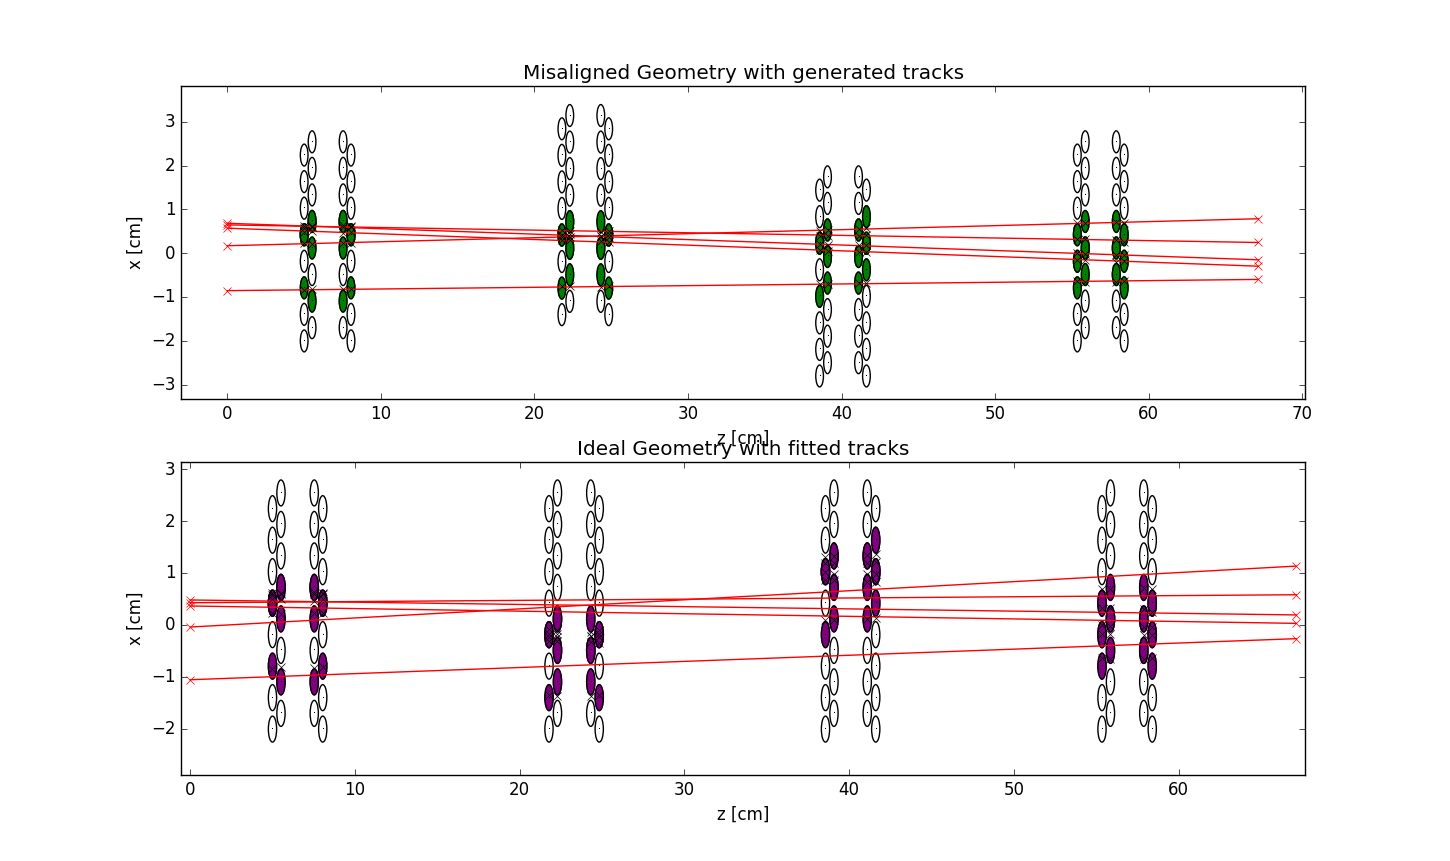
\includegraphics[width=1.0\textwidth]{Alignment}
				\label{fig:Alignment}
			\end{figure}

		In a similar vein, the current track fitting incorporates an azimuthally symmetic 2D magnetic field when fitting tracks for the different trackers. This ignores the full 3D field and any differences between the trackers. (Eg. There is no radial field in the simulation currently.) The effects might be negligible, or it might be necessary to include these differences for proper tracking results. It should be on others to calculate, measure, and add these fields to the gm2 simulation, but it will be necessary to update the field setting code in GeaneParamUtils.cc to implement them in the fitting.

	\subsection{Small dcas}

		As seen in \href{https://gm2-docdb.fnal.gov/cgi-bin/private/ShowDocument?docid=6171}{DocDB 6171} the uncertainty in the dca value measured in a straw when a particle passes close to the wire ($\textless{}500 \mu m$) is large. For this reason such measurements will be set to the wire center with a larger error. There is code available to do this as described in the \hyperref[sec:GeaneLRUtils]{GeaneLRUtils} section, which has been shown to work. However, exactly what this threshold should be set at, and its combination with the Garfield errors as described above have yet to be implemented. It's important to do this right for correct tracking results, as even a single measurement in a track with incorrectly assigned errors can throw the whole track off.

	\subsection{5x5 fitter}

		Deepak Sathyan has created the 5x5 fitter as detailed in the Geane manual, as opposed to my more complex full fitter which includes the material correlations. The first results from it are shown in \href{https://gm2-docdb.fnal.gov/cgi-bin/private/ShowDocument?docid=6950}{DocDB 6950} though improvements have been made since then. It can be seen that the results are actually very similar to those from the full fitter. The code itself lives in Deepak's repository on the gm2 machines, and has not been officially added to the feature/trackDevelop branch of the git repository. For speed reasons it will be a good idea to perform the first iterations of the track fitting with this 5x5 fitter which is faster than the full fitter, and only use the full fitter for the laster iteration or so. This should speed up the code significantly without harming physics results.

	\subsection{Commissioning data}

		The June 2017 commissioning run for Muon g-2 gathered some very useful data for the trackers. Some of the data and resulting fitted tracks are detailed in \href{https://gm2-docdb.fnal.gov/cgi-bin/private/ShowDocument?docid=6992}{DocDB 6992}, \href{https://gm2-docdb.fnal.gov/cgi-bin/private/ShowDocument?docid=7463}{DocDB 7463}, and \href{https://gm2-docdb.fnal.gov/cgi-bin/private/ShowDocument?docid=7571}{DocDB 7571}. While there is an extent to the usefulness of the data gathered during the commissioning run due to the prevalence of protons, and there is a wealth of work that needs to be done to improve the tracking, it would still be beneficial to examine the commissioning data more thoroughly. Doing so could reveal features that the data exhibits that simulation does not, point to bugs or insufficiencies in the tracking code, teach about the tracking in general, etc. Certainly examining this data will be a nice preparation for the data that will come in starting in November and beyond.

	\subsection{Further left-right work}

		As detailed in the \hyperref[sec:GeaneLRUtils]{GeaneLRUtils} and \hyperref[sec:LR]{Left-Right} sections a good amount of work has been done regarding handling the left-right ambiguities of the straw measurements within the track fitting. However this code can certainly be expanded and improved to deal with this better and faster. When updates to the track finding code have been made upstream to help deal with this left-right problem, those updates also need to be integrated with the local Geane fitting code. Further studies beyond \href{https://gm2-docdb.fnal.gov/cgi-bin/private/ShowDocument?docid=6800}{DocDB 6800} should also be conducted in order to optimize the tracking results vs speed.

	\subsection{Refinement}

		At the time of writing this, the ``Refinement'' stage of the track reconstruction has not been started. This refinement stage has the job of refining the track by adding hits, removing hits, updating errors, making improvements to left-right guesses, updating T0, and more. While not a direct part of the Geane fitting code, this stage will take information from the Geane fitting results, do its work, and then loop back and refit the track. For this reason, there will be a great deal of work that needs to be done regarding this refinement stage in the future. Be aware that this work will take a very long time (both the updates to the local Geane fitting code and the general refinement stage coding), probably on the order of a year or more, but is a necessary addition to the whole track reconstruction.

	\subsection{Short track fitter}

		Tracks which hit a smaller number of planes naturally fit worse with greater uncertainty on the fitted track. There is a hard cutoff in the upstream reconstruction chain at 6 planes hit. There is a noticeable difference in the fit of tracks that hit 7 or 8 planes vs 9 or more. This is because tracks that hit 7 or 8 planes in adjacent modules have a smaller track length which makes fitting the momentum more difficult. However if those 7 or 8 planes are spread out among modules separated by larger distances then the fit can still be good. This is something to be kept in mind when looking at fitting results.

		For tracks with 6 or less planes hit however, the hard cutoff has been in place since the development of the Geane fitting code. Because a good number of muons will decay close to the calorimeter and curve sharply through 6 or less planes it will be necessary to be able to fit these ``short'' tracks. The Geane fitting code should technically be able to handle these short tracks, though the results will certainly be worse, and this needs to be studied. Separately, and maybe with more priority, a specialized short track fitter will probably need to be written.

	\subsection{Geane extrapolation}

		After the track fitting stage comes the extrapolation stage, where the fitted track is extrapolated back into the storage region in order to determine the muon beam profile. Saskia Charity has developed the extrapolation code that we've been using. With the goal of having more than one version of every stage of the track reconstruction code however, we'll need a second track extrapolator at some point. The Geant4 Geane error propagation routines provide a nice and straightforward way to do this, which is why I've included a note about it here even though it is not directly related to the Geane fitting. One can pull out and modify the relevant code described in the \hyperref[sec:GeaneParamUtils]{GeaneParamUtils} file to do this. Deepak Sathyan has started this but it requires more work going forward.

	\subsection{Optimization}

		While mentioned in the intro to this section, I thought I'd quickly mention optimization. The Geane fitting code like all others needs to be optimized in pretty much all ways. Memory and speed can certainly be improved, maybe even by an order of magnitude or so. I have done very little work regarding this part of the code. Deepak Sathyan quickly and easily improved the track fitting speed by 5x, the first results of which are shown in \href{https://gm2-docdb.fnal.gov/cgi-bin/private/ShowDocument?docid=7094}{DocDB 7094}. More can and needs to be done.

	\subsection{Miscellaneous}

		I'll mention a couple smaller pieces of work here that shouldn't be forgotten.

		In the track fitting, the tungsten wires within the gas should be removed (and just replaced with gas). Due to the uncertainty in the fitted track, it isn't clear whether the track would have gone through a wire or not. If it does in the error propagation however, then a large number is added to the error due to passing through the tungsten material, which is not something we want to include.

		When completing wire fits (very useful for data), there is a discreteness to the results since there is only so many combinations of wires that can be hit. (And a set of hit wires will reconstruct exactly the same track for a wire fit.)  This discreteness and its effects should probably be studied in a little more detail, as they seem to introduce some slightly weird effects in the tracking results, as shown in \href{https://gm2-docdb.fnal.gov/cgi-bin/private/ShowDocument?docid=7463}{DocDB 7463}. Not only that but its possible that this discreteness might be taken advantage of by using some sort of quick look up table to shortcut the wire fit for a known set of wires, per James Mott's suggestion.




\printbibliography

\section{Acknowledgements}

	I'd like to a thank a number of people who helped me in this track fitting work, without whom this would not have been possible. Since this is not my thesis and more of a technical document, I will keep it brief though these people deserve more words. Thanks to Lee Roberts for the opportunity to work in physics on Muon g-2 and the constant support. Thanks to Rob Carey for the introduction to this project, and the constant advice and input. Thanks to Rob Kutschke for being a source of tracking expertise. Thanks to Joe Price for help with the code. Finally, thanks to James Mott for the endless patience, advice, direction, day-to-day help, and support, without which I believe I would have given up long ago.

\appendix
\section{Appendix}
\label{sec:Appendix}

  \subsection{Angular correction}

  Our straws don't actually measure U and V coordinates directly, but instead measure the distance of closest approach radii deriving from measured hit times. In order to utilize the minimization procedure on measured track parameters these radii must first be converted to U and V parameters, and similarly for the U and V errors. (Note that a future Kalman filter will not be subject to this disadvantage.) This is done in the calcMeasuredParams method at the bottom of the GeaneParamUtils class. These conversion corrections will be dependent on the angle of the track, so it's imporant to note that during each successive iteration, the ``measured'' parameters are adjusted by the latest ``predicted'' momenta. It was found that for the error correction, a simple straight line correction was sufficient for ideal results. For the position correction, it was found that a constant field correction for curved tracks was sufficient.

  To calculate these corrections, first the momentum perpendicular to the straw measurement axis can be ignored since it won't affect the U or V value. Because the positron tracks curve in only one direction through the tracker, one needs to calculate the correction depending on whether the track went to the left or right side of the wire. See Figure \ref{fig:angularCorrection} for a pictorial representation of the problem. The calculation of the right side correction follows, with the left side correction being calculated in a similar manner.

	\begin{figure}[]
	\caption{Shown here is a positron passing through a straw. The desire is to convert the measured parameter d into a U or V position, which can be done by approximating the particle trajectory as a circle in a constant magnetic field over the course of the straw and using trigonometry. Sizes and angles are exaggerated.}
	\centering
	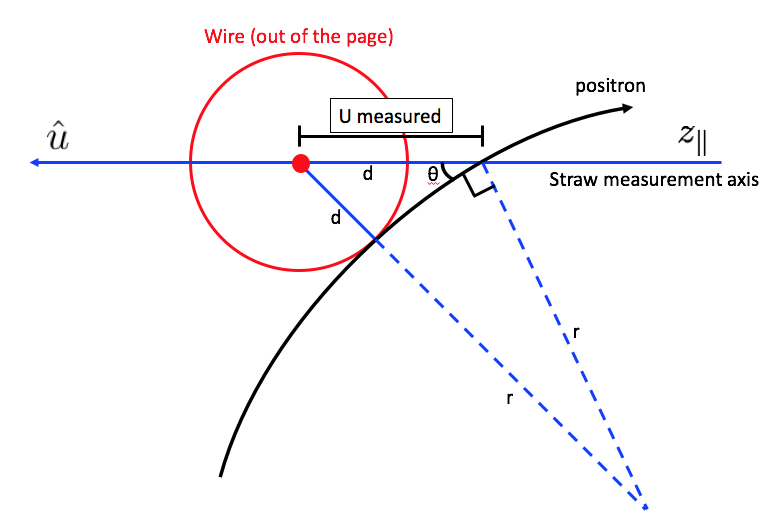
\includegraphics[width=1.0\textwidth]{angularCorrection}
	\label{fig:angularCorrection}
	\end{figure}

  To solve for the measured U (or V) value, we can use the equation:
	\begin{align}
		(r+d)^{2} = r^{2}+u^{2}-2ru\cos(90+\theta),
	\end{align}
  where the 90 degrees is approximate for large curvature of tracks. The angle $\theta$ can be determined from 
	\begin{align}
		\hat{z_{\parallel}} \cdot \hat{p_{\parallel}} = \cos{\theta}, \hspace{.1cm} \theta = \cos^{-1}{\frac{p_{\parallel}}{p}}, 
	\end{align}
  where $p_{\parallel}$ is the positron momentum parallel to the $z_{\parallel}$ axis at the wire plane and can be determined within the code. (The $z_{\parallel}$ axis simply stands for the axis perpendicular to the straw and parallel to the U measurement axis, but opposite in direction. At the end this calculated U value will simply be added or subtracted to the wire center U position depending on which side of the wire the positron travelled.) Using some trig identities and solving for u gives
	\begin{align}
		u = -r\sqrt{1-(\frac{p_{\parallel}}{p})^{2}} + \sqrt{d^{2} + 2dr + r^{2}(1-(\frac{p_{\parallel}}{p})^{2})},
	\end{align}
  for the right side correction, and 
	\begin{align}
		u = +r\sqrt{1-(\frac{p_{\parallel}}{p})^{2}} - \sqrt{d^{2} + 2dr + r^{2}(1-(\frac{p_{\parallel}}{p})^{2})},
	\end{align}
  for the left side correction. (Corrections to v are identical.) The radius of the particle circle can be calculated from the circular momentum and magnetic field at the predicted hit position. The straightline correction is done simply using the Pythagorean theorem in a simpler manner, with the correction to the errors then being
	\begin{align}
		\sigma_{uv}' = \frac{\sigma_{uv}}{\sqrt{1-(\frac{p_{\parallel}}{p})^{2}}}.
	\end{align}


\subsection{Matrix Transformation}
\label{sec:MatTransf}

  Transport matrices are accumulated as
      \begin{align} %\label{eq:nolabel}
        T_{mn} = T_{mk}T_{kn},
      \end{align}
  where the indices can stand for either plane numbers or step numbers, and converted by 
      \begin{align} %\label{eq:nolabel}
        T_{mn,s} = A_{m} T_{mn,f} A_{n}^{-1},
      \end{align}     
  where the indices s and f stand for the surface and free trajectory states respectively, and A is the Jacobian transformation from the free state to the surface state on a particular plane m or n. See \cite{jacob} for the calculation of these Jacobians. The error matrices in the surface state can be grabbed directly from the Geant code unlike the transport matrices, or if necessary can be converted as
      \begin{align} %\label{eq:nolabel}
        \sigma_{m,s} = A_{m} \sigma_{m,f} A_{m}^{-1}.
      \end{align}  



\subsection{GEANEArtRecord.hh} 
\begin{longtable}{|p{16cm}|}
% \scriptsize
\caption{GEANEArtRecord.hh active variables. This is subject to change. GEANEArtRecord contains vectors of variables on planes, as well as larger objects containing information about the whole track. Note that Eigen matrix objects cannot be stored into art data products. For this reason, and for minimal code changes, it was decided to add a data object for each Eigen member, made up of vectors with the word ``Data'' tagged at the end. The data objects are saved when creating GEANEArtRecords using a utils file. In analyzers accessing the GEANEArtRecords, these data objects are then swapped into the Eigen objects using the same utils file.}
 
\label{tab:artRecord}

% \begin{tabular}{|p{16cm}|}

  \\ \hline

enum GeaneHitSide \\ 
\textit{An enum for which side of the wire the track hit is guessed or calculated to have passed. Options are gLeft, gRight, gCenter, gNA\_side, and gUnknown. The first three are self explanatory, gNA\_side simply means there wasn't a hit, and gUnknown is used within the LR sequence checking part of the fitting code where any hits with said value or looped over to try and find the best choice.} 

  \\ \hline

art::Ptr \textless{} gm2strawtracker::TrackCandidateArtRecord \textgreater{} candidate \\
\textit{One track corresponding to one candidate corresponding to one GEANEArtRecord for the whole track.} \\ \hline

std::vector\textless{} art::Ptr\textless{} gm2truth::GhostDetectorArtRecord \textgreater{} \textgreater{} dummyPlaneHits \\
\textit{Associated dummy plane hits on planes aligned with straw wires, vector consists of hit dummy planes corresponding to hit wire planes (if a straw plane was skipped but that dummy plane was hit, it is not included in this vector. Vector has size N = num hits in straws that form the track +1 for the 0 plane.)} \\ \hline

int failureMode \\ 
\textit{Different failure modes for failed track reconstruction, 0 means it passed.} \\ \hline

double chi2 \\ 
\textit{Chi2 for whole track.} \\ \hline

std::vector\textless{}double\textgreater{} chi2Iterations \\
\textit{Chi2s for whole track for different iterations.} \\ \hline

std::vector\textless{}double\textgreater{} chi2Planes \\
\textit{Individual chi2s on each plane which add up to total chi2, vector consists of hit planes with size N.} \\ \hline

int numIterations \\
\textit{Number of iterations to converge.} \\ \hline

unsigned int dof \\
\textit{DoF of track = number of hit planes - 5 track parameters.} \\ \hline

double chi2DoF \\
\textit{chi2/dof} \\ \hline

double pValue \\
\textit{Fit pValue for whole track.} \\ \hline

double energyDiff \\
\textit{energy loss between first and last hit in track - from truth, for material characterizing} \\ \hline

std::vector\textless{}double\textgreater{} startingTrackParameters \\
\textit{Starting parameters for track: size 6, 3 position then 3 momentum, x y z px py pz, best starting parameters updated after each iteration, starting parameters x position defined before first hit.} \\ \hline

std::vector\textless{}double\textgreater{} startingTrackGuessOffsets \\
\textit{Size 10, x y z px py pz p 1/p pu/px pv/px offsets in different starting track parameters for plotting purposes.} \\ \hline

int trackNumPlanesHit \\ 
\textit{Total number of planes hit.} \\ \hline

int trackFirstPlaneHit \\ \hline

int trackLastPlaneHit \\ \hline

std::vector\textless{}int\textgreater{} trackPlanesHitList \\
\textit{List of hit planes, with missed planes excluded from the vector. Ex. 1 2 4 5 8 9} \\ \hline


std::vector\textless{}std::vector\textless{}double\textgreater{} \textgreater{} wireUVPositions \\
\textit{Wire center U and V postions, first vector is track param vector size 5 (0 1 2 unfilled, 3 is U, 4 is V), second vector is planenumber from 0 - 32  (formatted this way to align with other similar vectors - can probably be reduced.)} \\ \hline

std::vector\textless{}double\textgreater{} measuredDCAs \\
\textit{Vector of measured DCAs for hit planes, with size 33. Mainly to hold on to smearing values for now.} \\ \hline

std::vector\textless{}double\textgreater{} UVerrors \\
\textit{Vector of UV measurement errors for planes 0-32. Built in order to accomadate varying errors in the future.} \\ \hline

std::vector\textless{}double\textgreater{} planeXPositions \\
\textit{Vector of X postions of hit wire planes with size 33 (0 - 32), 0 plane being in front of the first module that was hit.} \\ \hline

std::vector\textless{}std::vector\textless{}double\textgreater{} \textgreater{} geaneMeasuredParameters \\
\textit{Measured GEANE parameters, first vector is param num 0 - 4, second vector is plane number 0 - 32, units are MeV mm. 1/P, Pu/Pz, Pv/Pz, U, V - only U or V is filled at the start of the GEANE fitting module.} \\ \hline

std::vector\textless{}std::vector\textless{}double\textgreater{} \textgreater{} geanePredictedParameters \\ 
\textit{Predicted GEANE parameters, first vector is param num 0 - 4, second vector is plane number 0 - 32, units are MeV mm. 1/P, Py/Px, Pz/Px, Y, Z - all params filled in tracing stage of GEANE fitting module - coord system has to be orthogonal - converted to UV locally in the fitting module.} \\ \hline

std::vector\textless{}GeaneHitSide>\textgreater{} geaneHitSides \\
\textit{Vector of GeaneHitSide enums with size 33 describing the sides of the wires that each hit of the track passed.}
 

std::vector\textless{}Eigen::MatrixXd\textgreater{} geaneTransportMatrices \\
std::vector\textless{}std::vector\textless{}double\textgreater{} \textgreater{} geaneTransportMatricesData \\ 
\textit{Units of GeV cm - transport matrices between planes tracked to in GEANE fitting module, 5x5 objects. Vector has size 33.} \\ \hline

std::vector\textless{}Eigen::MatrixXd\textgreater{} geaneErrorMatrices \\ 
std::vector\textless{}std::vector\textless{}double\textgreater{} \textgreater{} geaneErrorMatricesData \\ 
\textit{Error matrices on tracked to planes, units GeV cm, size 33.} \\ \hline

Eigen::MatrixXd covarianceTotalInverse \\
std::vector\textless{}double\textgreater{} covarianceTotalInverseData \\
\textit{5x5 inverse of total covariance matrix for track. Diagonals represent errors in 5 track paramaters on plane 0.} \\ \hline

std::vector\textless{}Eigen::VectorXd\textgreater{} paramPredictedInUVEigen \\ 
std::vector\textless{}std::vector\textless{}double\textgreater{} \textgreater{} paramPredictedInUVEigenData \\ 
\textit{Predicted parameters in UV space as an eigen object (converted from geanePredictedParameters above) for calculation convenience and some LR information storage. Order of vectors is switched here, first is planenum, second is paramnum, units are MeV mm.} \\ \hline

\textit{Objects below here are full track objects with larger sizes, held on to for fast sequence checking. Units GeV cm.} \\ \hline

std::vector\textless{}Eigen::MatrixXd\textgreater{} extendedTransportMatrixBegToEnd \\
std::vector\textless{}std::vector\textless{}double\textgreater{} \textgreater{} extendedTransportMatrixBegToEndData \\ 
\textit{Accumulated/combined transport matrices from starting plane to all following planes.} \\ \hline

Eigen::MatrixXd extendedCombinedTransportMatricesTranspose \\
std::vector\textless{}double\textgreater{} extendedCombinedTransportMatricesTransposeData \\
\textit{Transpose of larger eigen object composed of above begtoend transport matrices.} \\ \hline

Eigen::MatrixXd extendedReducedMatrix \\
std::vector\textless{}double\textgreater{} extendedReducedMatrixData \\ 
\textit{Total error correlation matrix, reduced to size NxN (N = num planes hit).} \\ \hline

Eigen::MatrixXd extendedReducedMatrixInverse \\ 
std::vector\textless{}double\textgreater{} extendedReducedMatrixInverseData \\
\textit{Inverse of above saved once for LR checking.} \\ \hline

Eigen::MatrixXd extendedModifiedReducedMatrix \\ 
std::vector\textless{}double\textgreater{} extendedModifiedReducedMatrixData \\
\textit{Reduced matrix from above that's going to be modified into a hybrid error matrix separately for U and V fits but that needs to be held onto for all sequences.} \\ \hline



std::vector\textless{}int\textgreater{} hitSidesCorrect \\
\textit{Vector of ints as to whether the sides that the track fitting guessed/calculated were correct or not - only available when truth is available. 1 for correct, 0 for no hit, and -1 for incorrect. Almost certainly temporary.} \\ \hline


  \hline

% \end{tabular}
\end{longtable}




\newpage
\section{Plots}
\label{sec:Plots}

Here is a section of common plots that were produced with the GeanePlots module. (This is not all-inclusive.) These plots were generated with the makeGEANEPlots.fcl file with version v7\_06\_01 for truthLRFit tracks. There is no plane number cut in these plots, but there is a truth energy cut of 3 MeV to cut out some poor events. The tracks these plots describe were generated starting with 7000 muons times 500 grid jobs, 3.5 M muons, with the mdc1.fcl file, resulting in approximately 140,000 tracks. All three trackers were included in the simulation, unnecessary geometry was omitted (such as calorimeters), the trajectory art records were not recorded, orphans were not tracked, and normal material was included. If checking out this documentations repository, then the analyzer root file is located in ``Images/MainPlots/gm2GEANE\_ana\_19831354\_1504040981.139.root''.

Branch and commit numbers used to generate these plots are listed below: \\

artg4 - feature/trackDevelop - ed5436 \\

gm2analyses - develop - b470cb7 \\

gm2dataproducts - feature/trackDevelop - 4fb1dc \\

gm2geom - feature/trackDevelop - c623aa9 \\

gm2ringsim - feature/trackDevelop - 9684d18 \\

gm2tracker - feature/trackDevelop - aa9239e \\

gm2util - feature/trackDevelop - 17b7856 \\

The sam-data-set names are ``nkinnaird\_documentation\_events\_mdc1\_reduced'' and \\
``nkinnaird\_documentation\_tracks\_truthLRFit'' for the events and tracks respectively.
Some more information including the locations of the sam-data-sets and root files are included in the directory: \\
``/pnfs/GM2/persistent/Tracking/nkinnaird/Documentation''

\begin{figure}
    \centering
    \begin{subfigure}[]{0.7\textwidth}
        \centering
        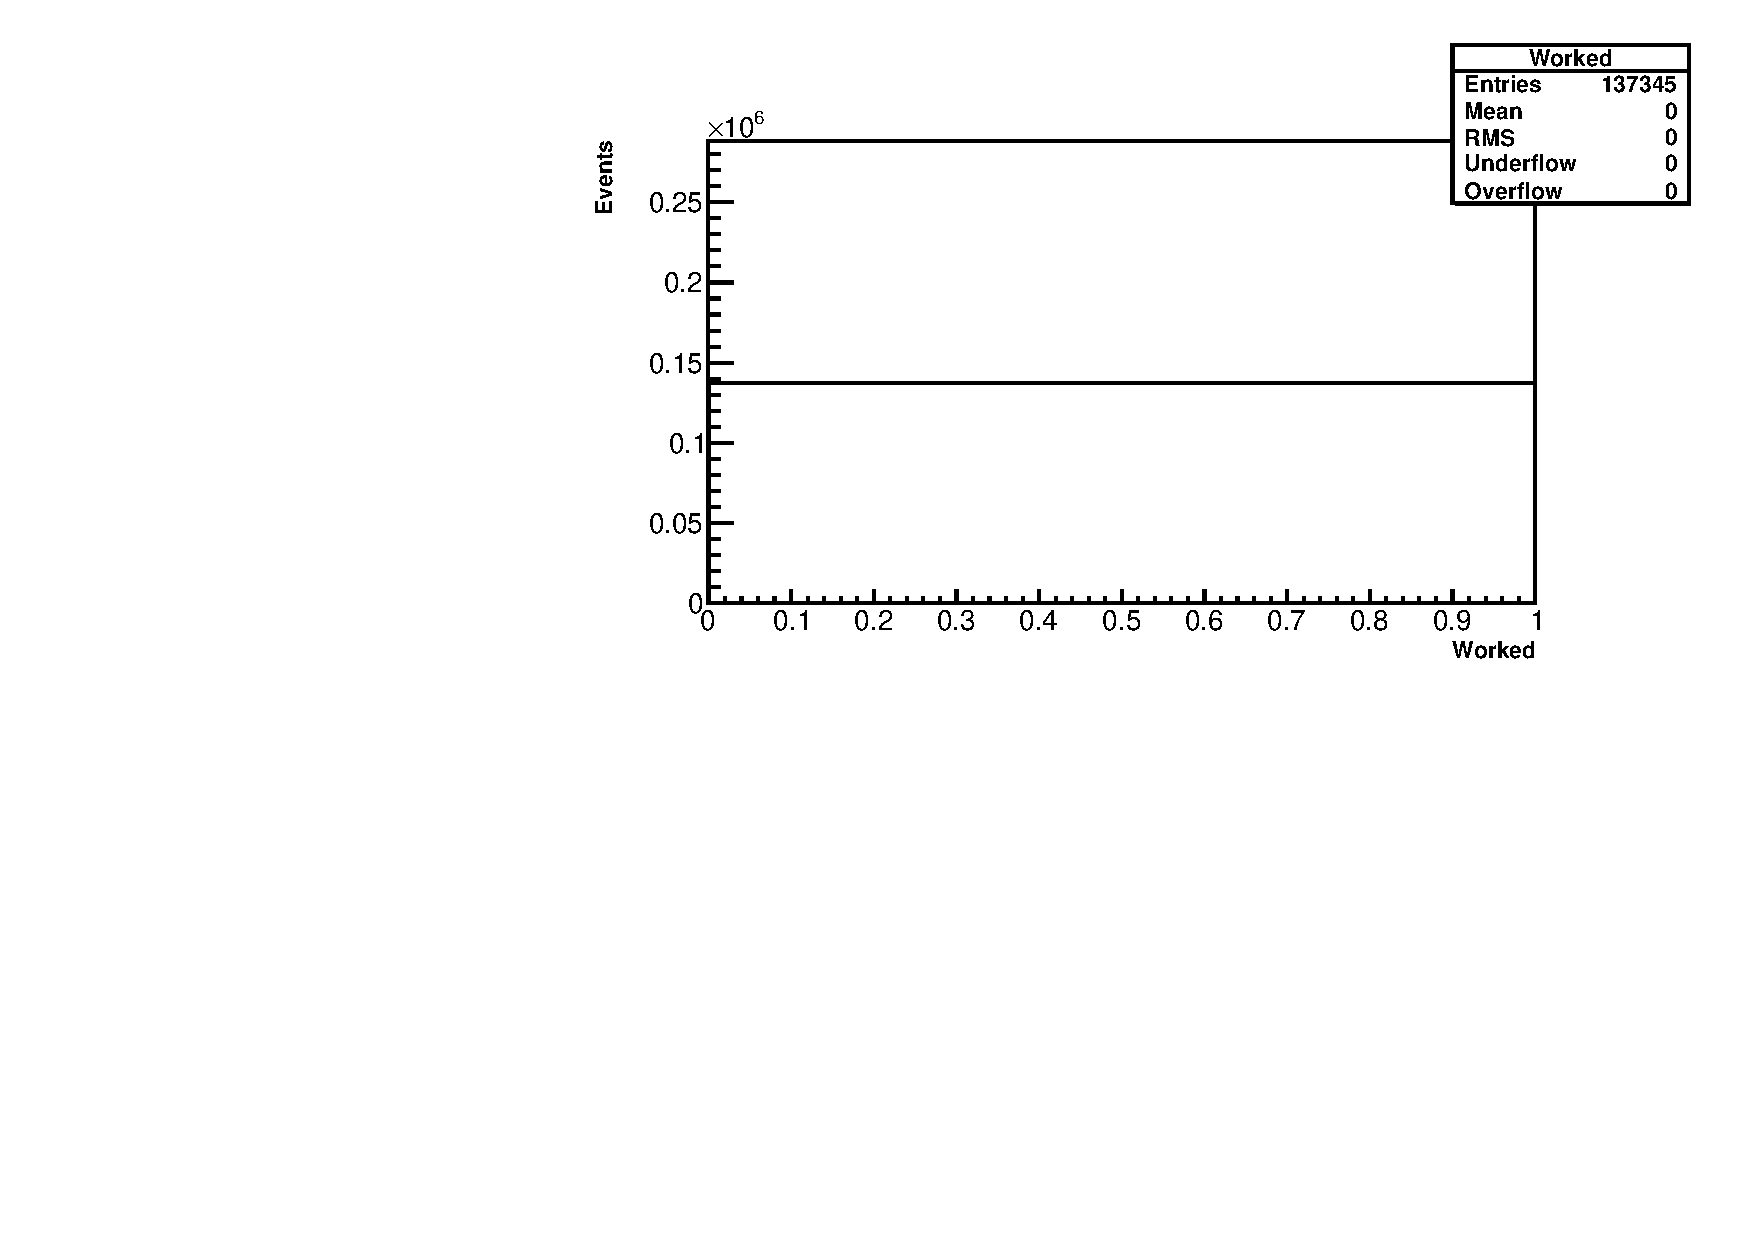
\includegraphics[width=1\textwidth]{WorkedEvents} 
        \caption{Number of events that passed the track fitting, with no cuts applied.}
        \label{fig:worked}
    \end{subfigure}
    
    \begin{subfigure}[]{0.7\textwidth}
        \centering
        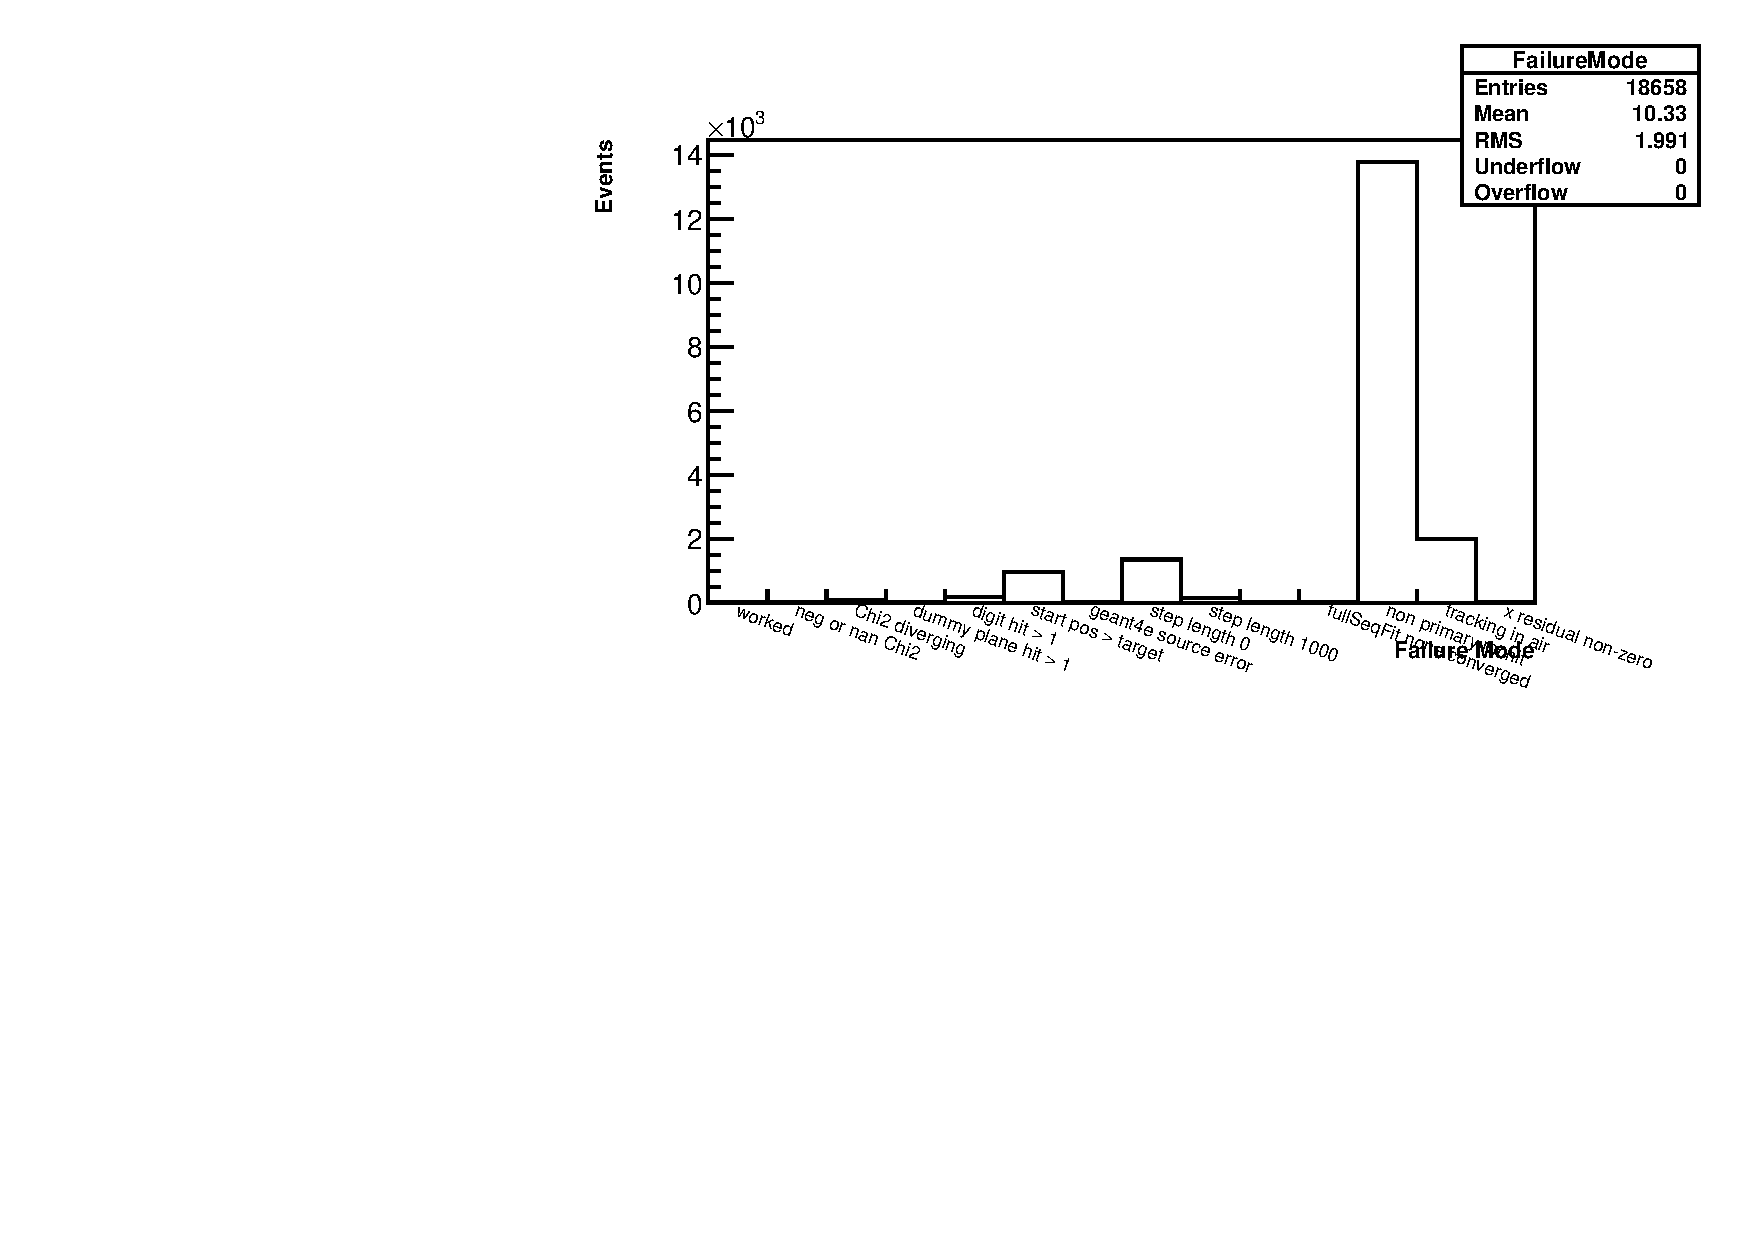
\includegraphics[width=1\textwidth]{FailedEventsUnzoomed} 
        \caption{Failure modes for the track reconstruction. Most ``failures'' are Geant issues.}
    \end{subfigure}

    \begin{subfigure}[]{0.7\textwidth}
        \centering
        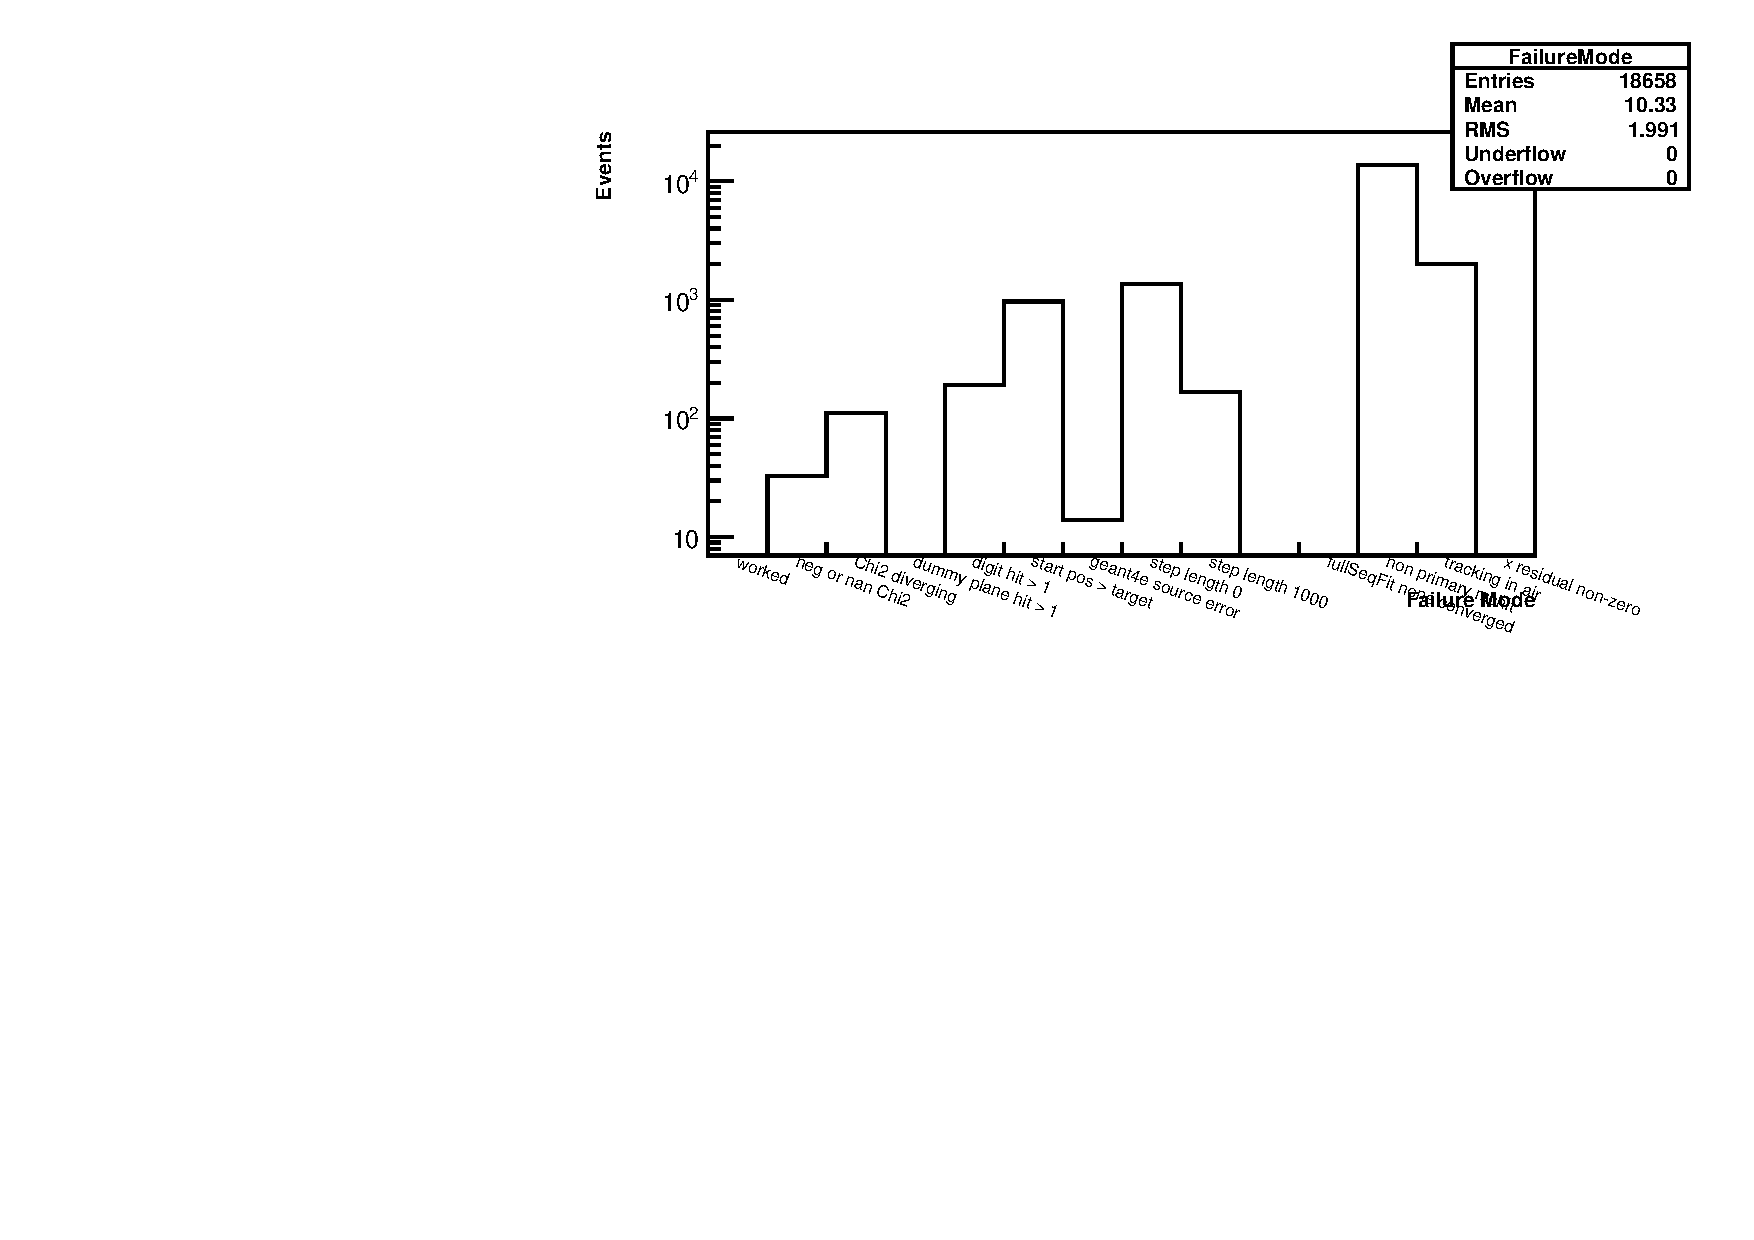
\includegraphics[width=1\textwidth]{FailedEventsLog} 
        \caption{Log plot of the failure modes. The first two failure mode bins are the most important.}
    \end{subfigure}

    \caption{The number of events that passed and failed the Geane track fitting.}
\end{figure}



\begin{figure}
    \centering
    \begin{subfigure}[]{0.7\textwidth}
        \centering
        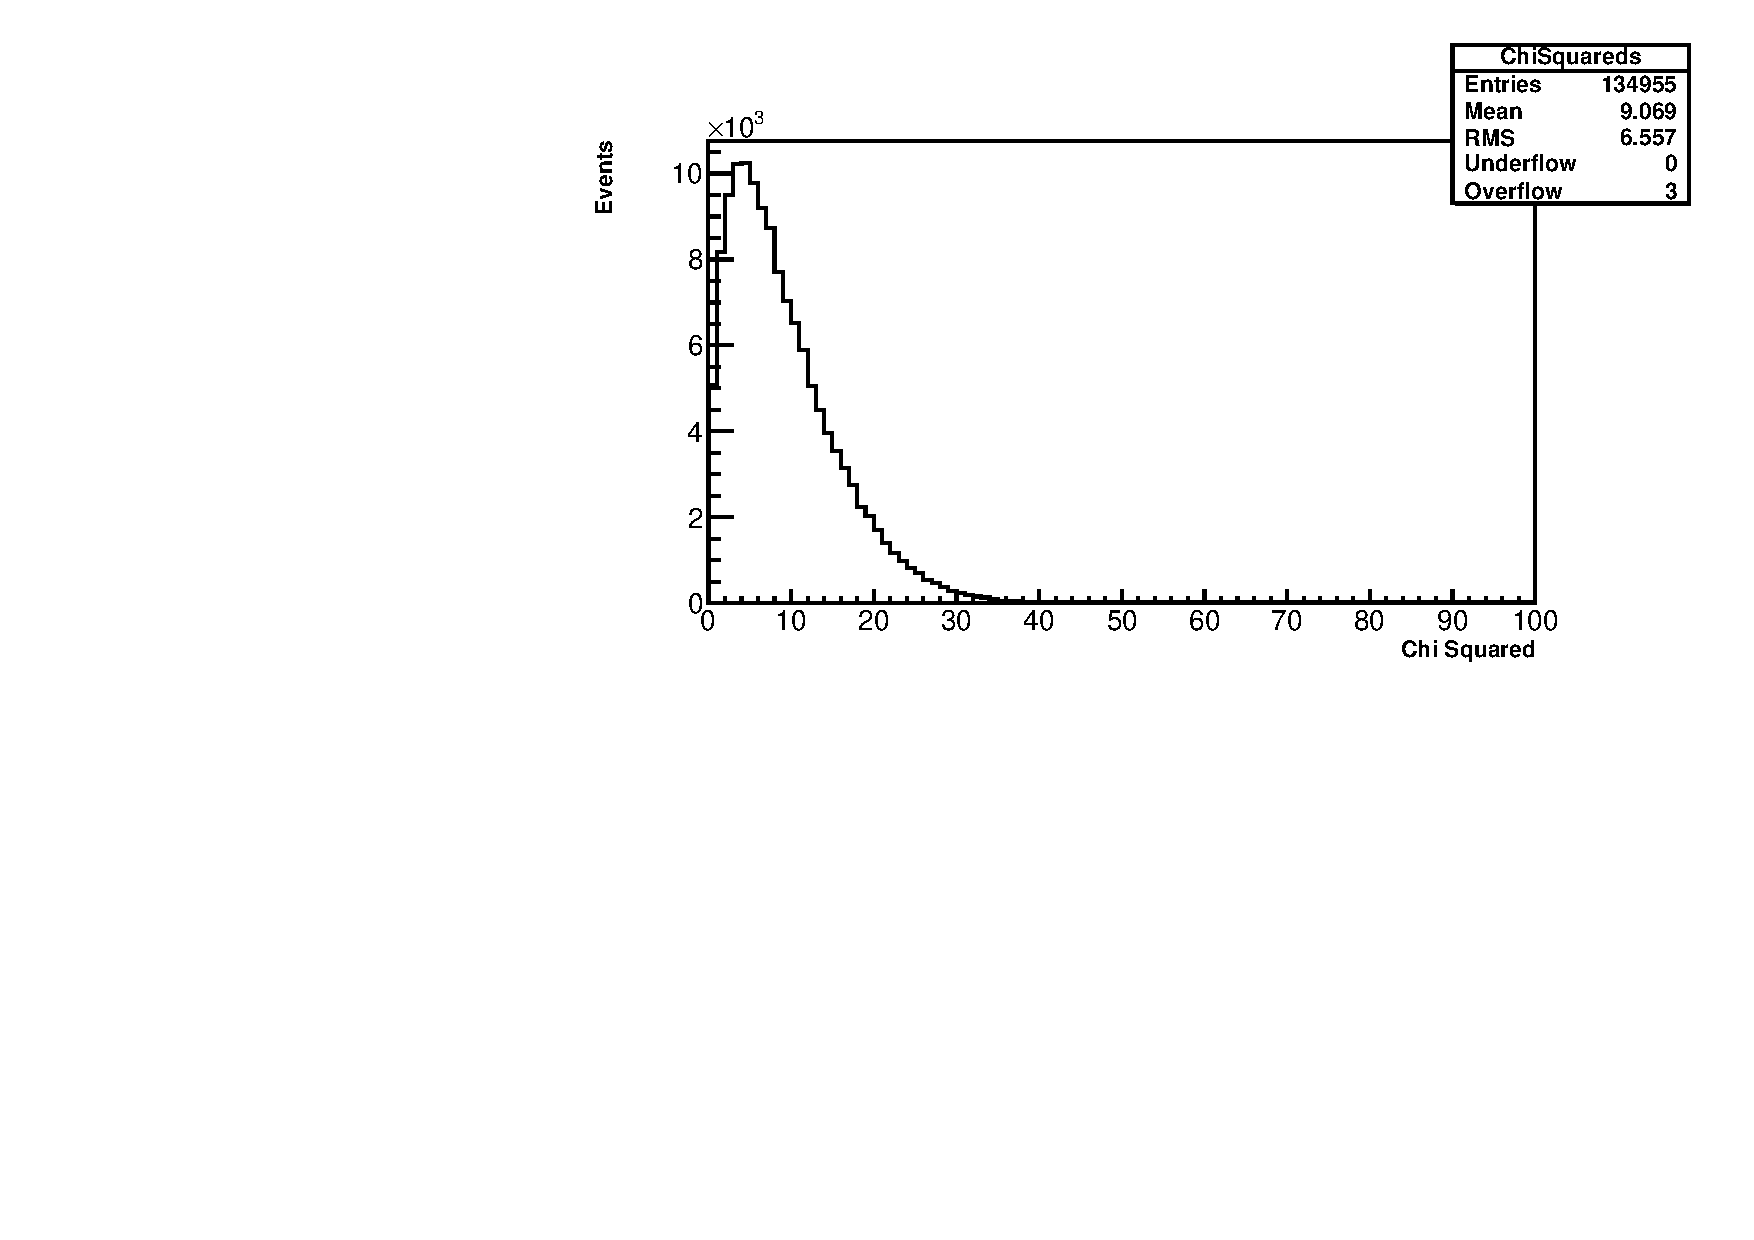
\includegraphics[width=1\textwidth]{chi2} 
        \caption{Distribution of $\chi^{2}$s for all tracks. Comprised of separate $\chi^{2}$ distributions with degrees of freedom equal to the number of planes hit minus 5.}
    \end{subfigure}
    
    \begin{subfigure}[]{0.7\textwidth}
        \centering
        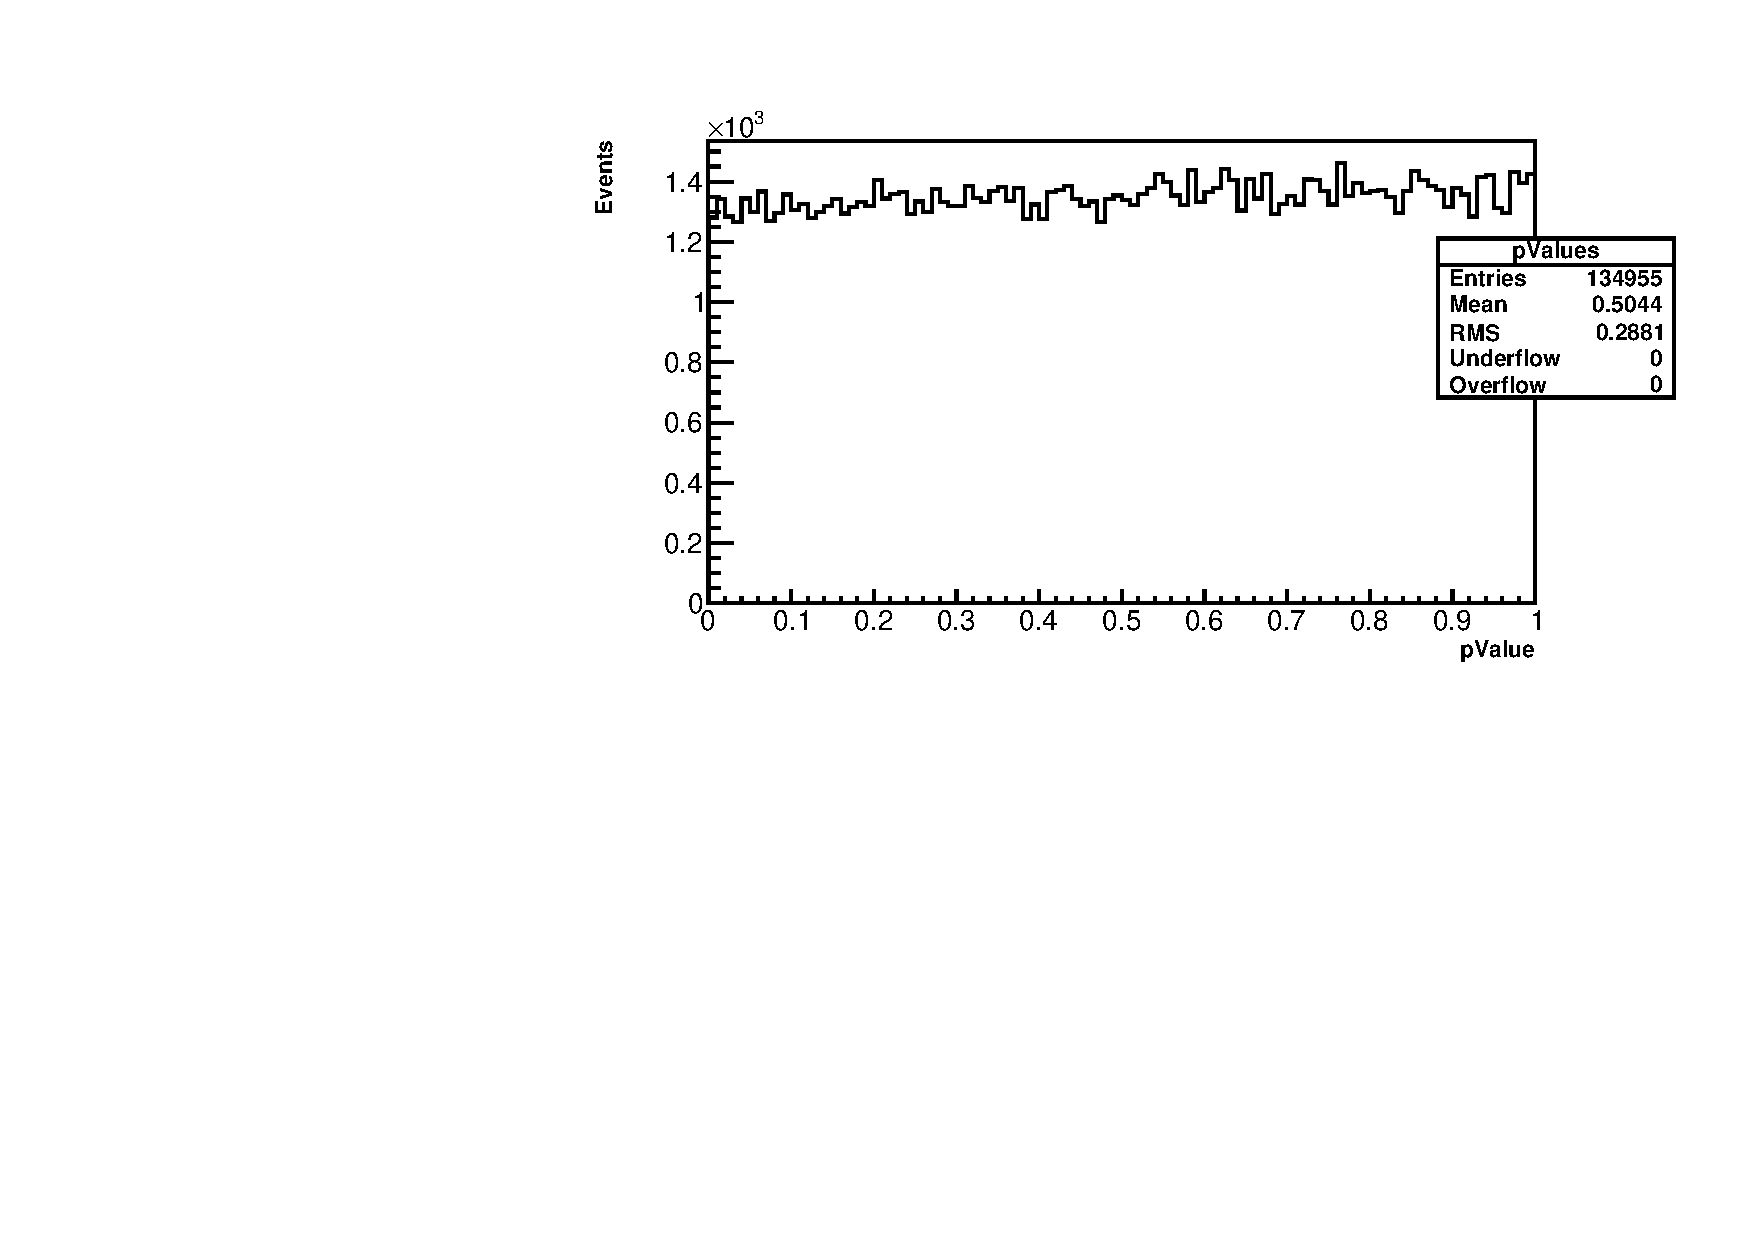
\includegraphics[width=1\textwidth]{pValueUnzoomed} 
        \caption{P-value distribution for tracks. Very nearly uniform, showing tracking is working as expected.}
    \end{subfigure}

    \begin{subfigure}[]{0.7\textwidth}
        \centering
        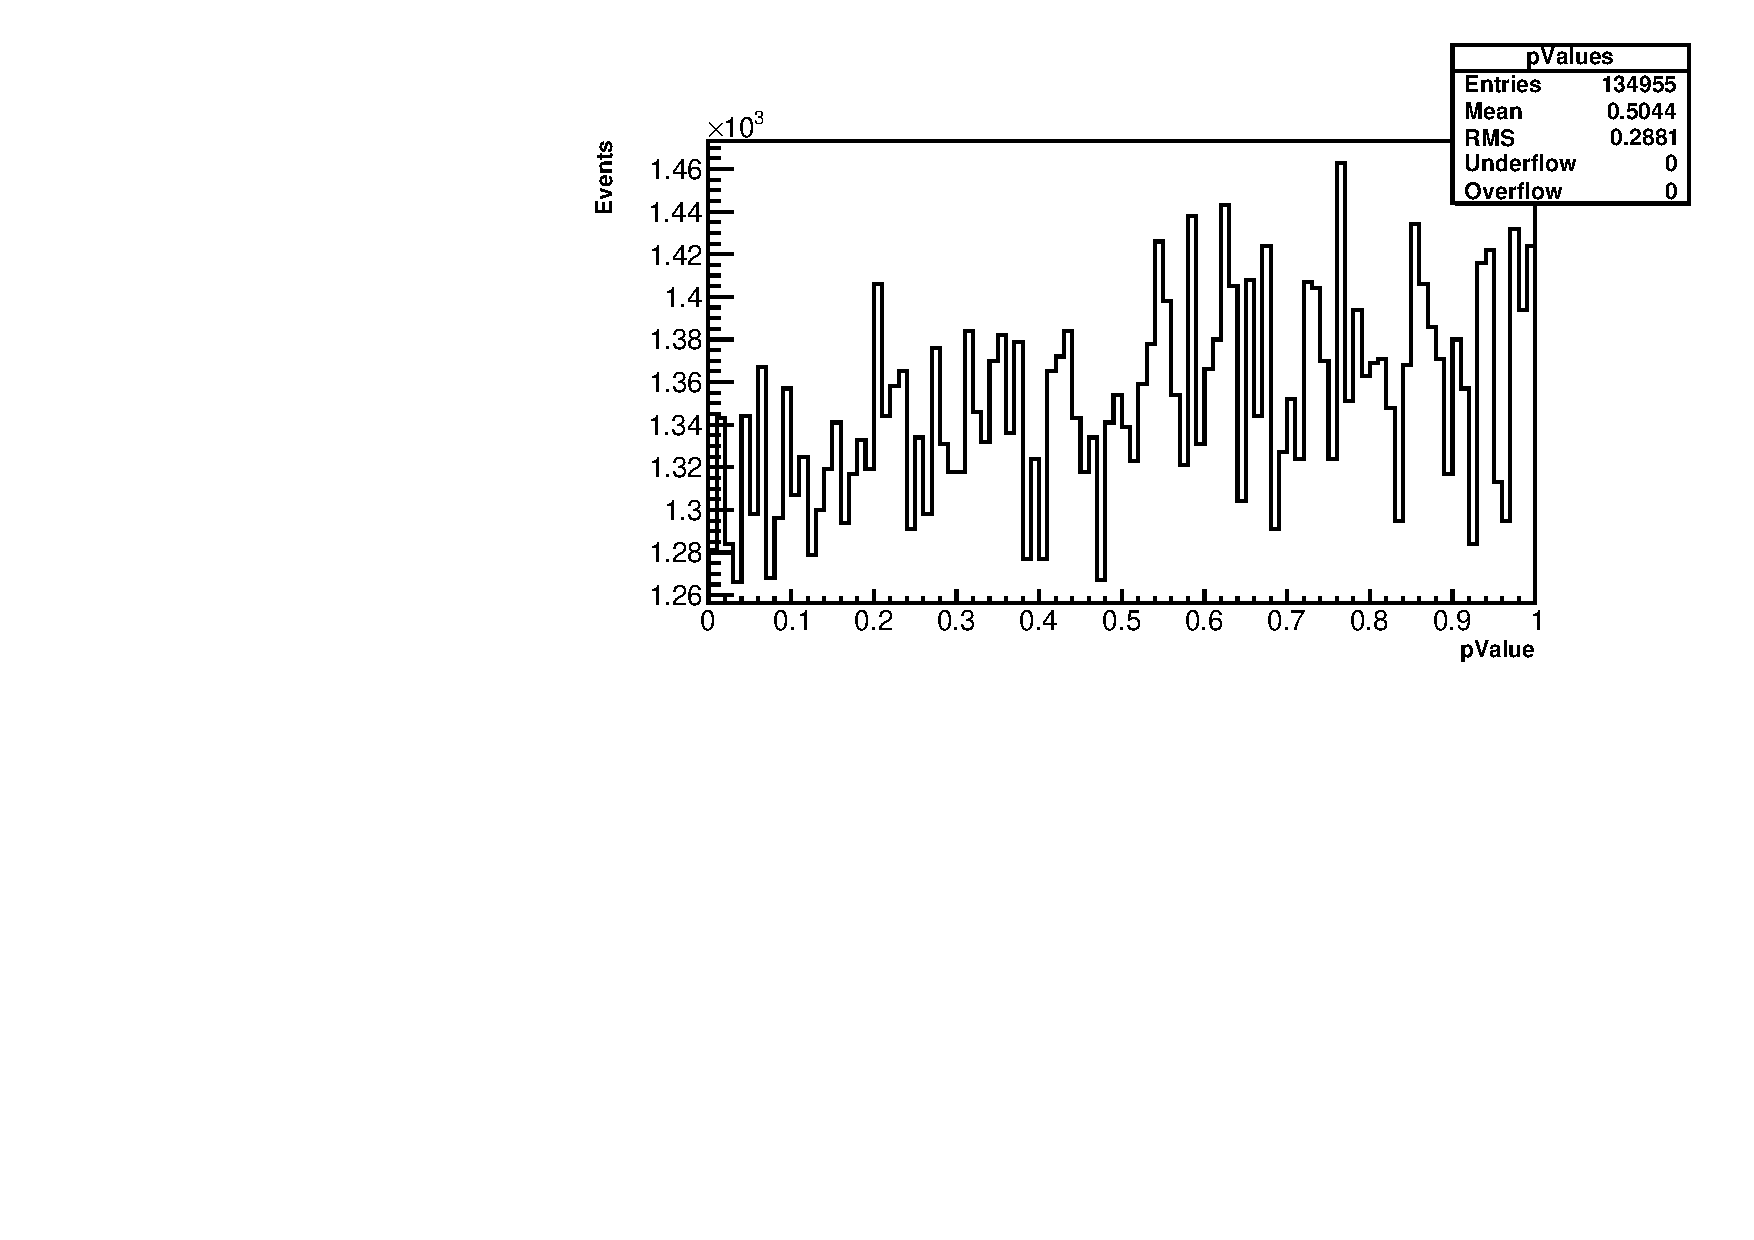
\includegraphics[width=1\textwidth]{pValueZoomed} 
        \caption{P-value distribution zoomed in. A slight rise towards 1 can be seen.}
    \end{subfigure}

    \caption{$\chi^{2}$ and p-value distributions for all tracks. There are less entries than in \ref{fig:worked} due to the energy cut of 3 MeV.}
\end{figure}



\begin{figure}
    \centering
    \begin{subfigure}[]{0.65\textwidth}
        \centering
        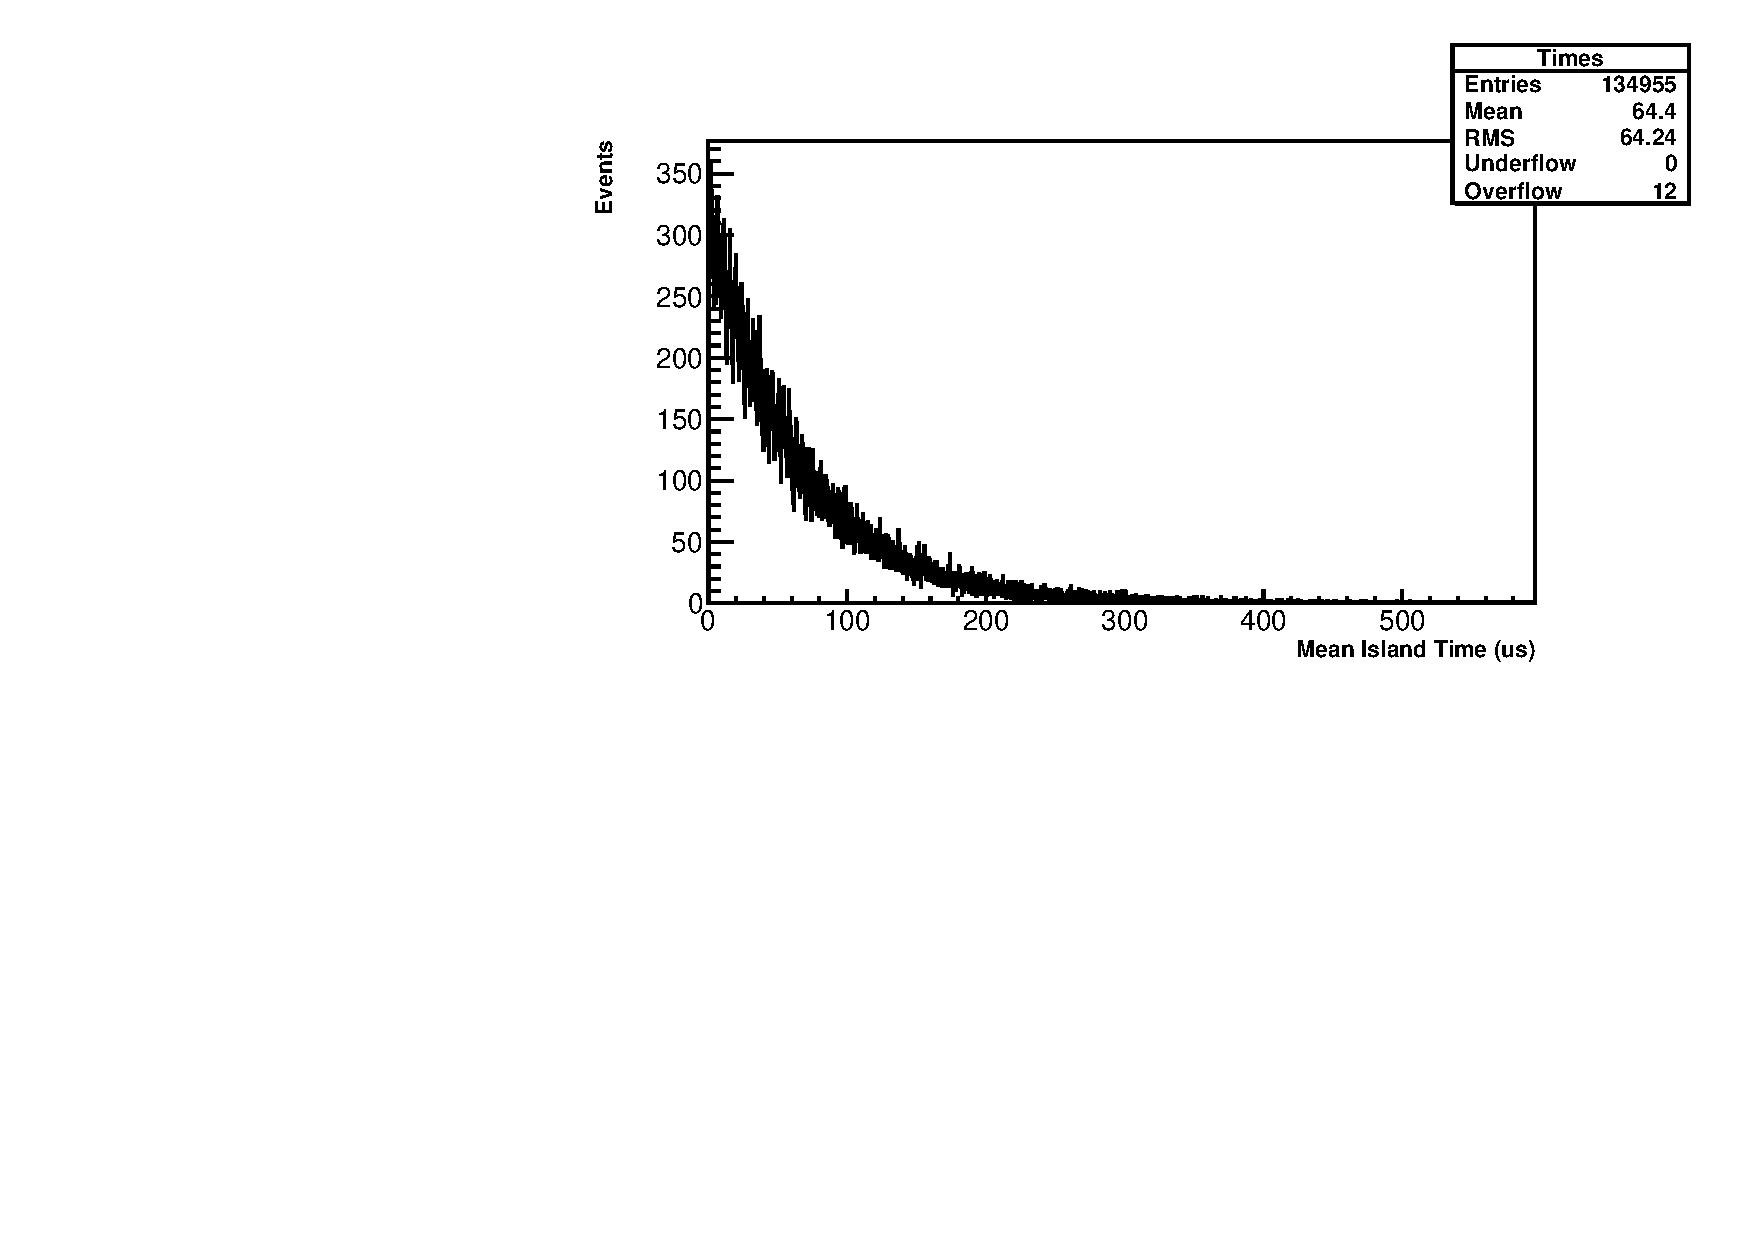
\includegraphics[width=1\textwidth]{Times} 
        \caption{Mean island times for fitted events from the mdc1 simulation. The cbo can just barely be seen.}
    \end{subfigure}
    
    \begin{subfigure}[]{0.65\textwidth}
        \centering
        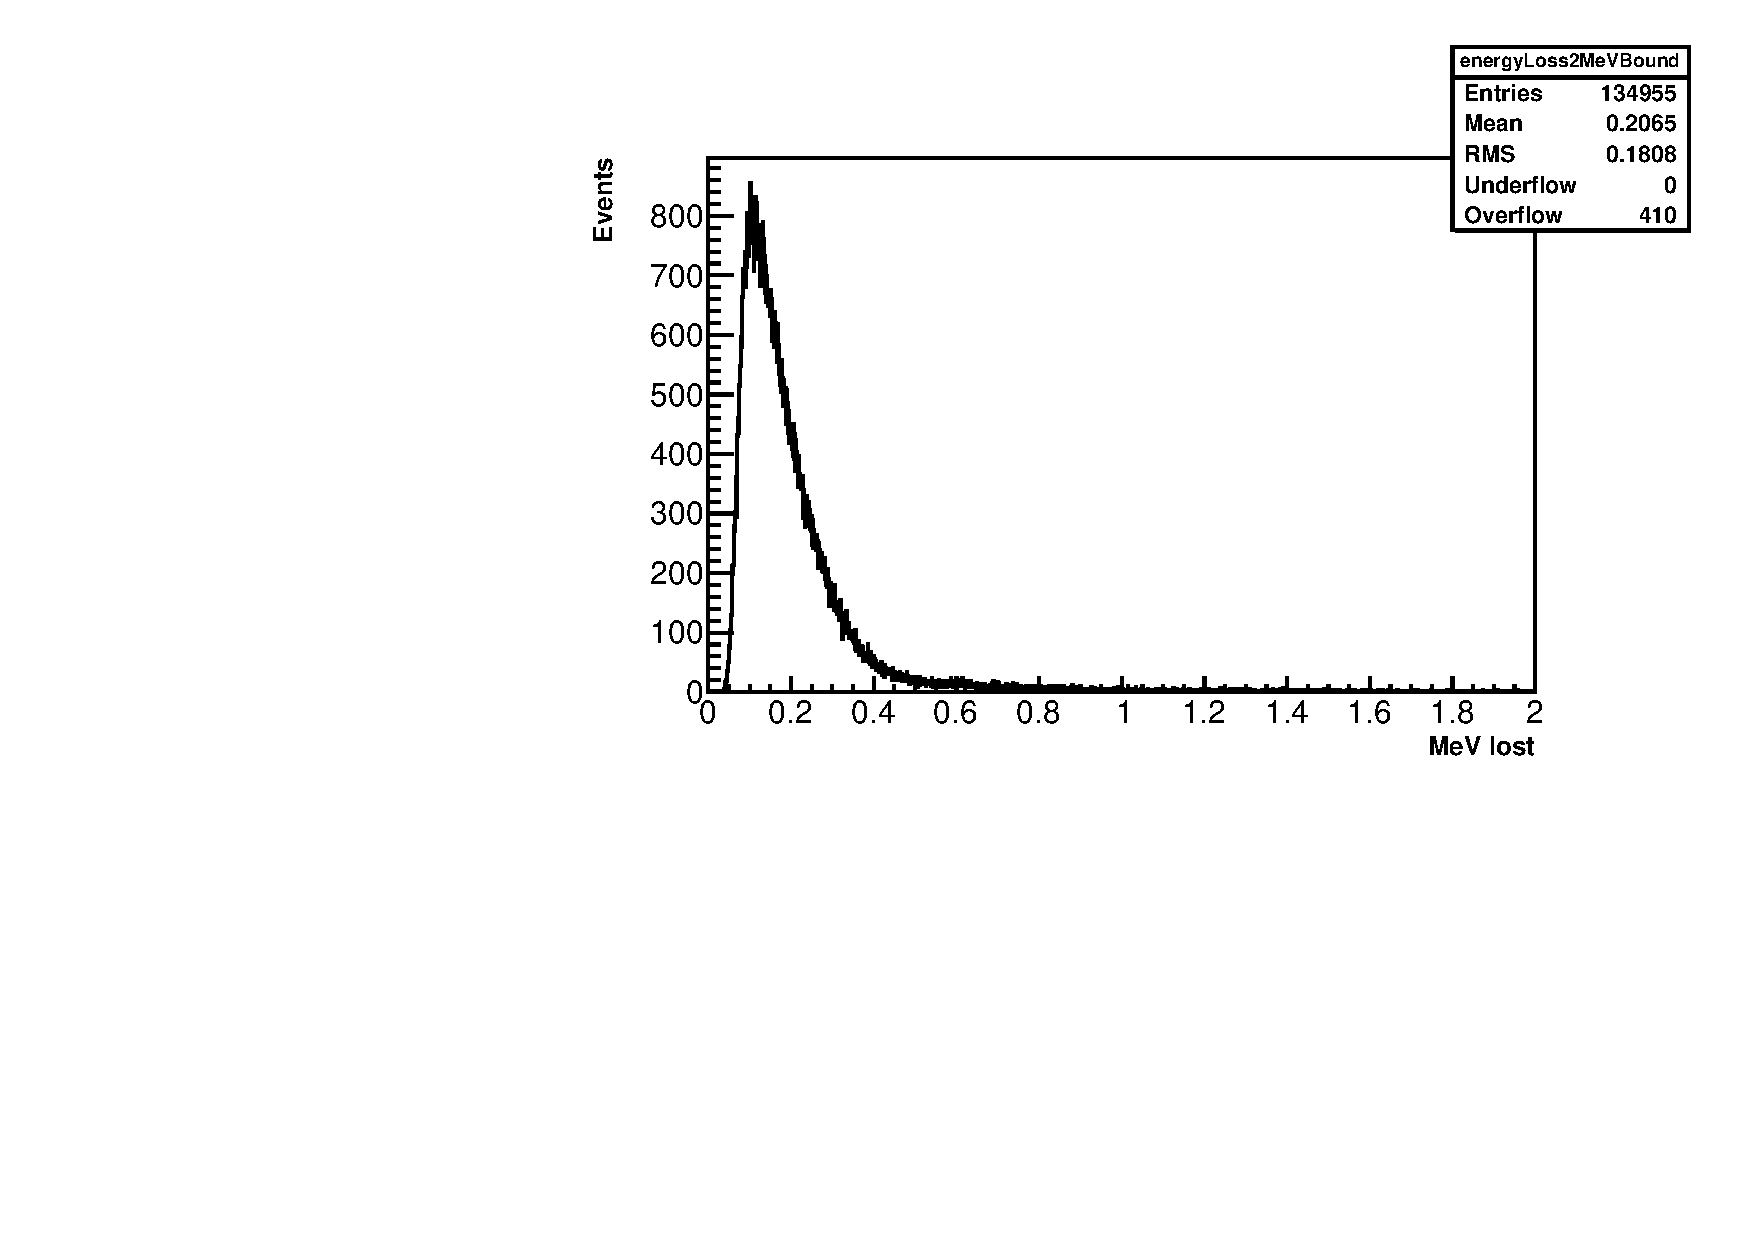
\includegraphics[width=1\textwidth]{trueEnergyLoss} 
        \caption{True energy loss between the first and last hit in the tracker. Peaks at about 120 keV with a mean of about 200 keV.}
    \end{subfigure}

    \begin{subfigure}[]{0.65\textwidth}
        \centering
        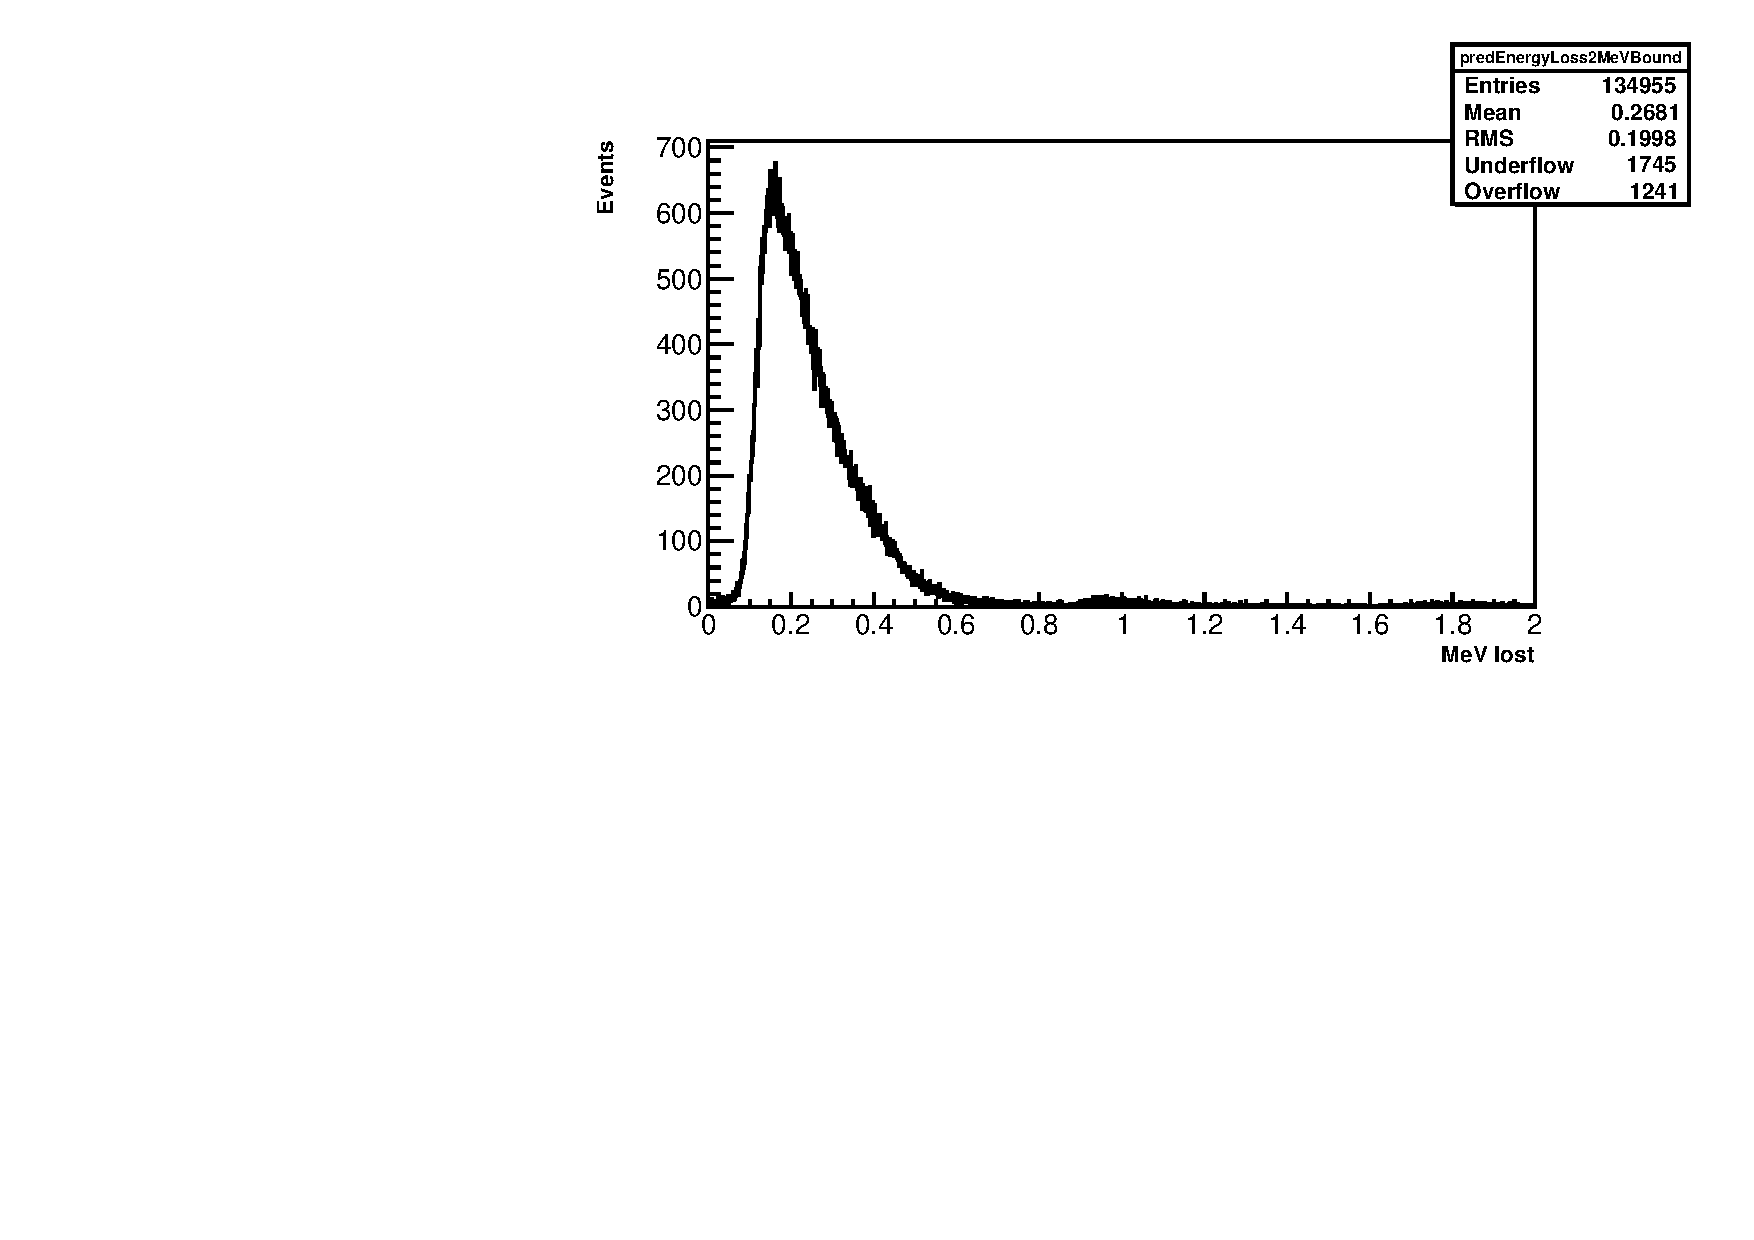
\includegraphics[width=1\textwidth]{predEnergyLoss} 
        \caption{Predicted energy loss from Geane fitting. Peaks at about 150 keV with a mean of about 270 keV. There is a slight overestimation of energy loss from truth. This is pretty negligble, but can probably be improved if necessary.}
    \end{subfigure}

    \caption{Energy and time information of the fitted tracks.}
\end{figure}



\begin{figure}
    \centering
    \begin{subfigure}[]{0.6\textwidth}
        \centering
        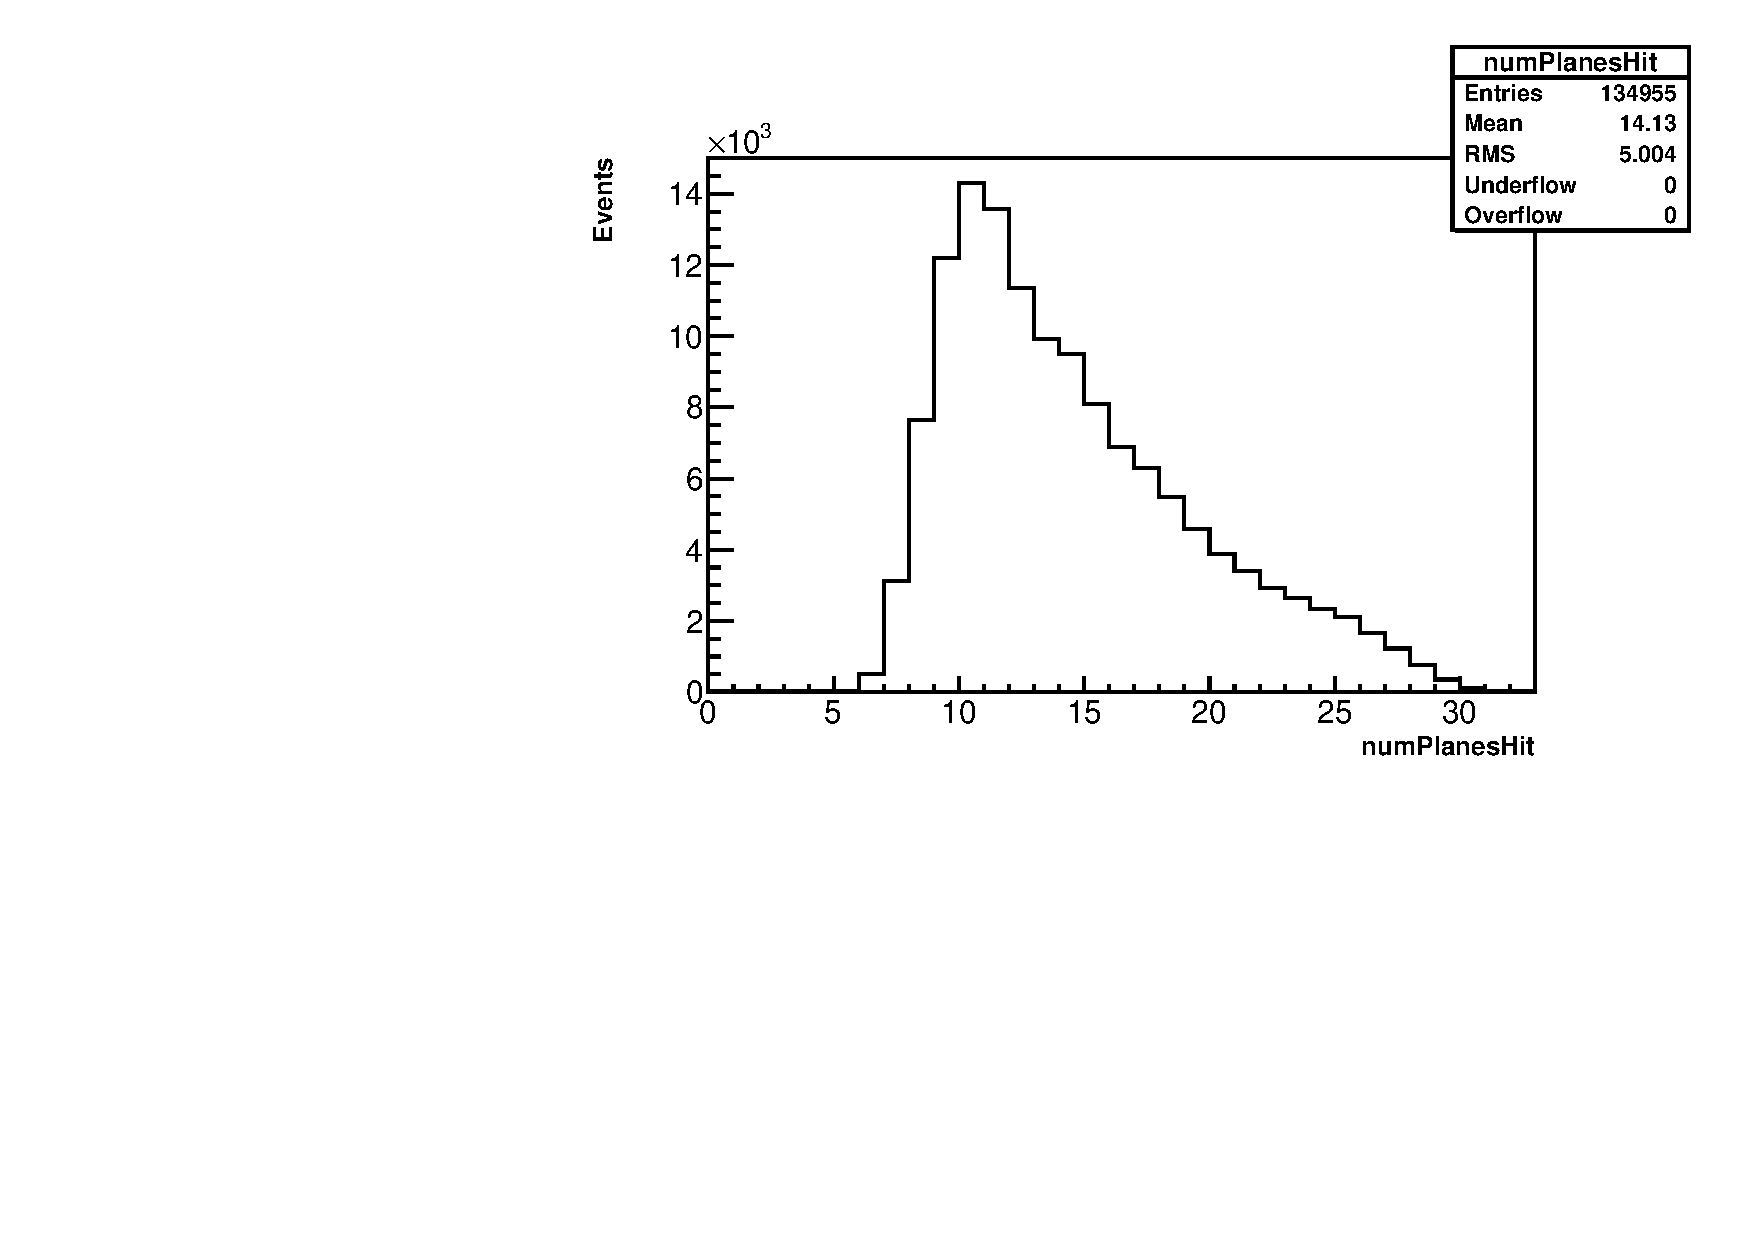
\includegraphics[width=1\textwidth]{numPlanesHit} 
        \caption{Number of planes hit per track. Peaks at 11 and falls off steadily.}
    \end{subfigure}
    
    \begin{subfigure}[]{0.6\textwidth}
        \centering
        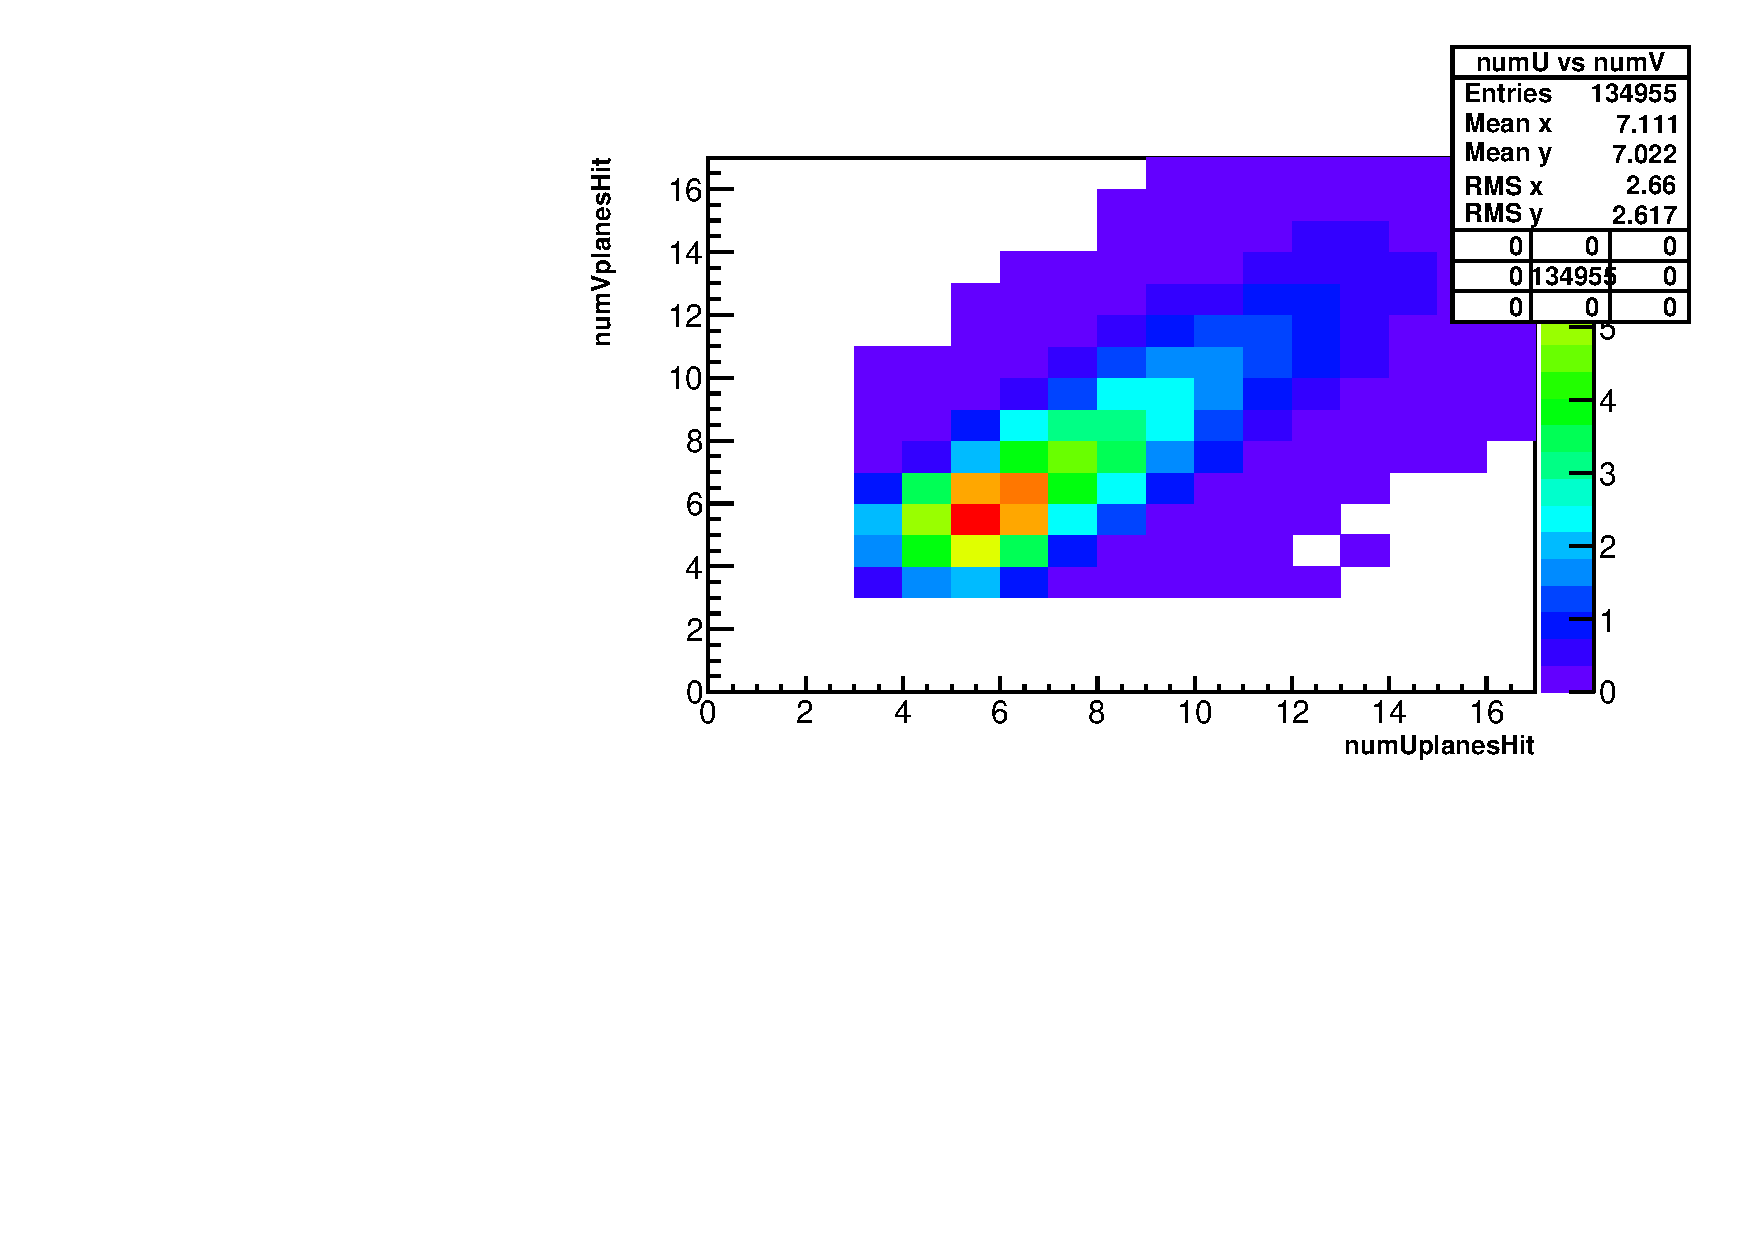
\includegraphics[width=1\textwidth]{numUnumV} 
        \caption{Number of U planes hit vs the number of V planes hit.}
    \end{subfigure}

    \begin{subfigure}[]{0.6\textwidth}
        \centering
        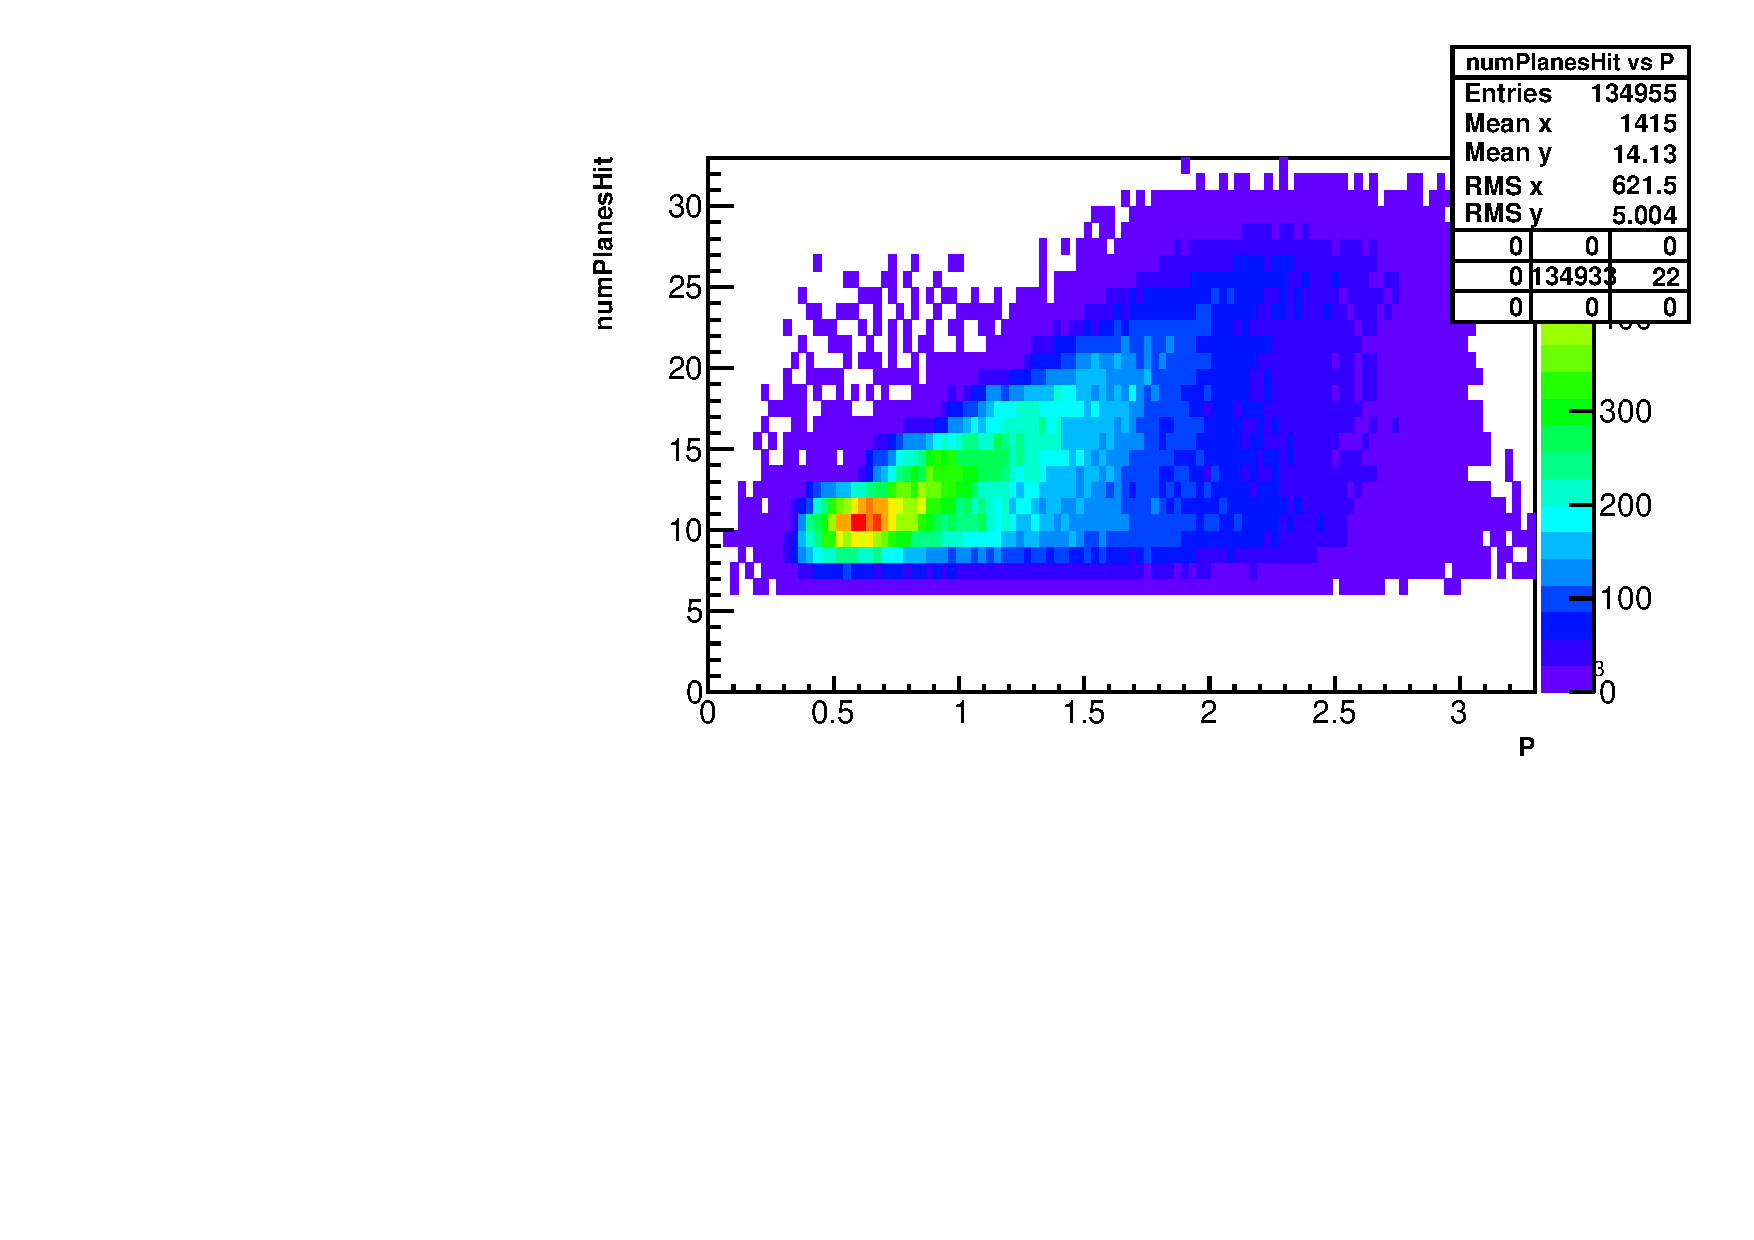
\includegraphics[width=1\textwidth]{numHitvsP} 
        \caption{Number of planes hit vs track momentum. These variables are very correlated, the higher the momentum of the track, the more likely it is to hit more planes.}
    \end{subfigure}

    \caption{Number of planes hit information.}
\end{figure}



\begin{figure}
    \centering
    \begin{subfigure}[]{0.8\textwidth}
        \centering
        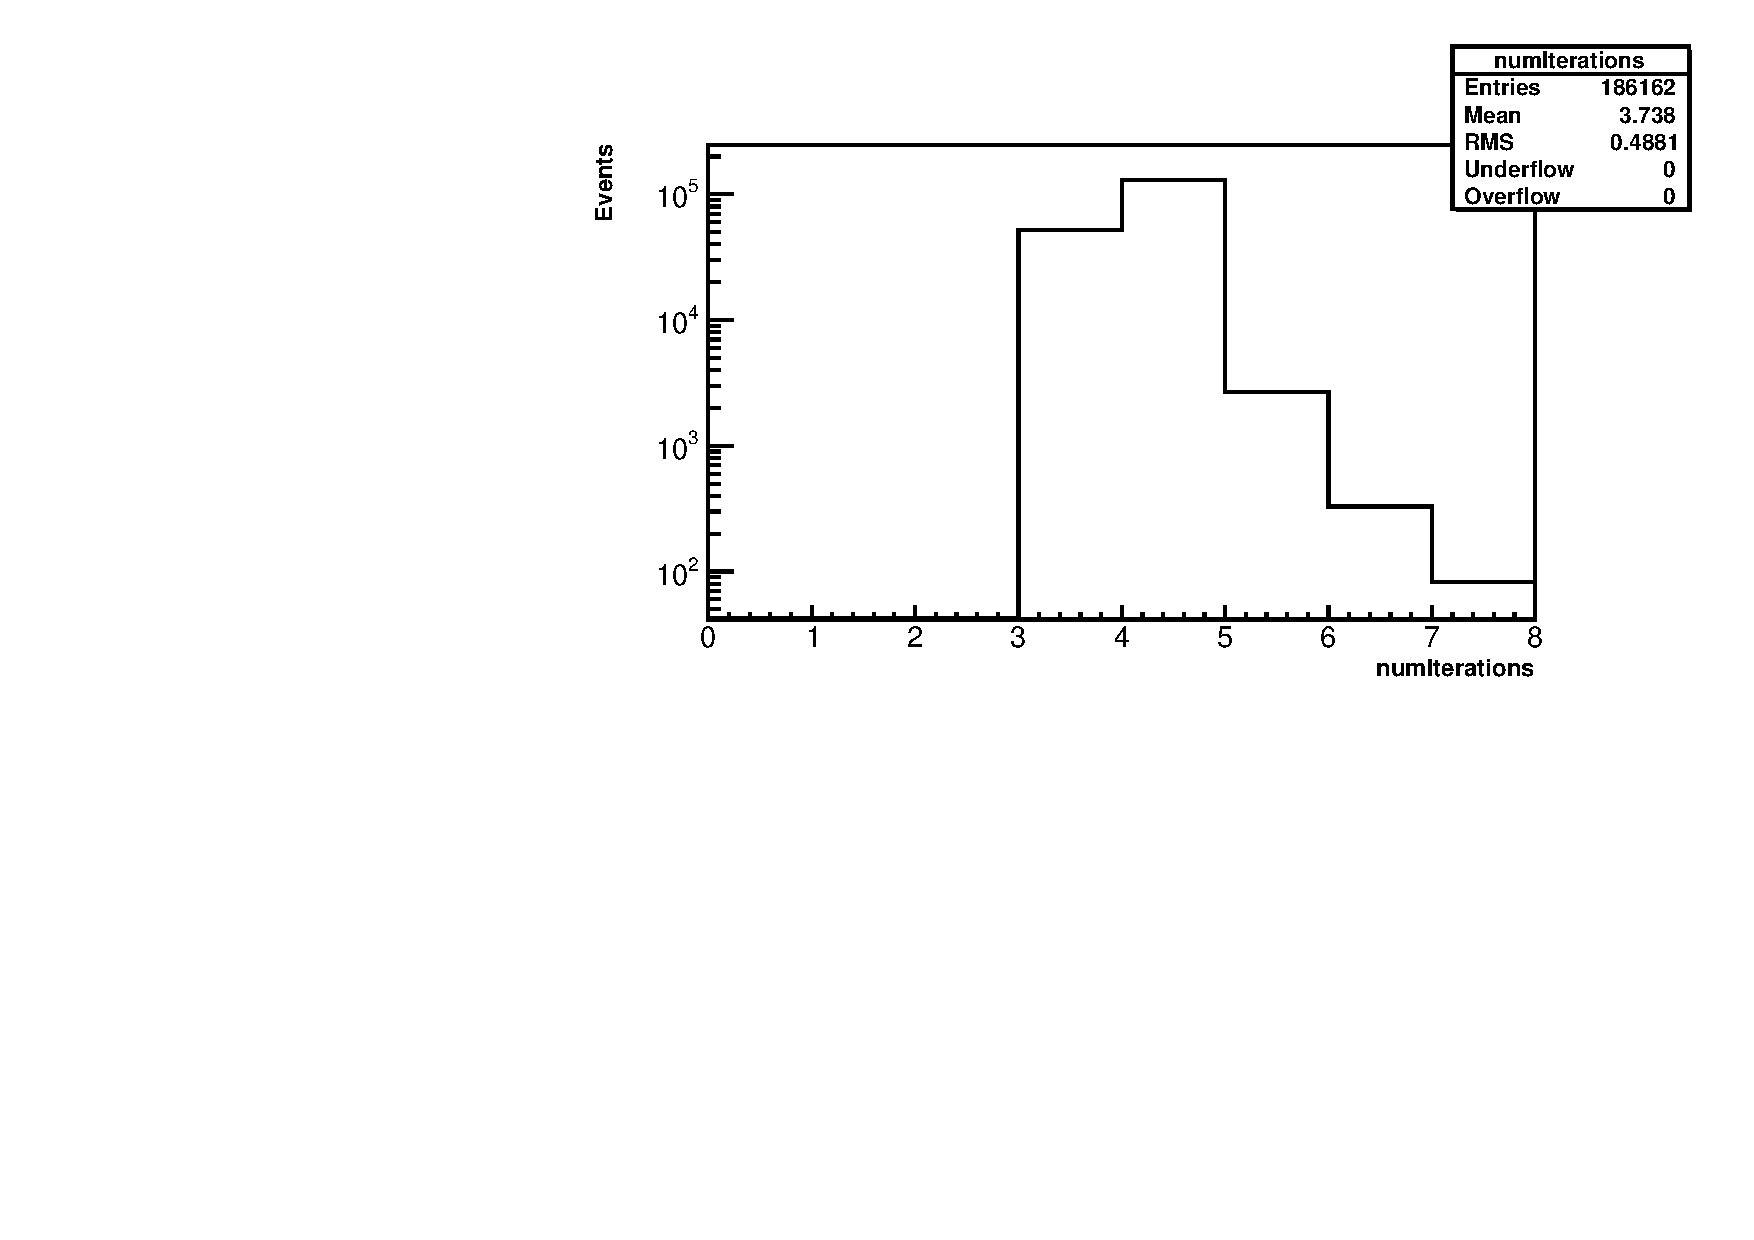
\includegraphics[width=1\textwidth]{numIterations} 
        \caption{Number of iterations to fit the track. Peaks at 4 with not less than 3 iterations.}
    \end{subfigure}
    
    \begin{subfigure}[]{0.8\textwidth}
        \centering
        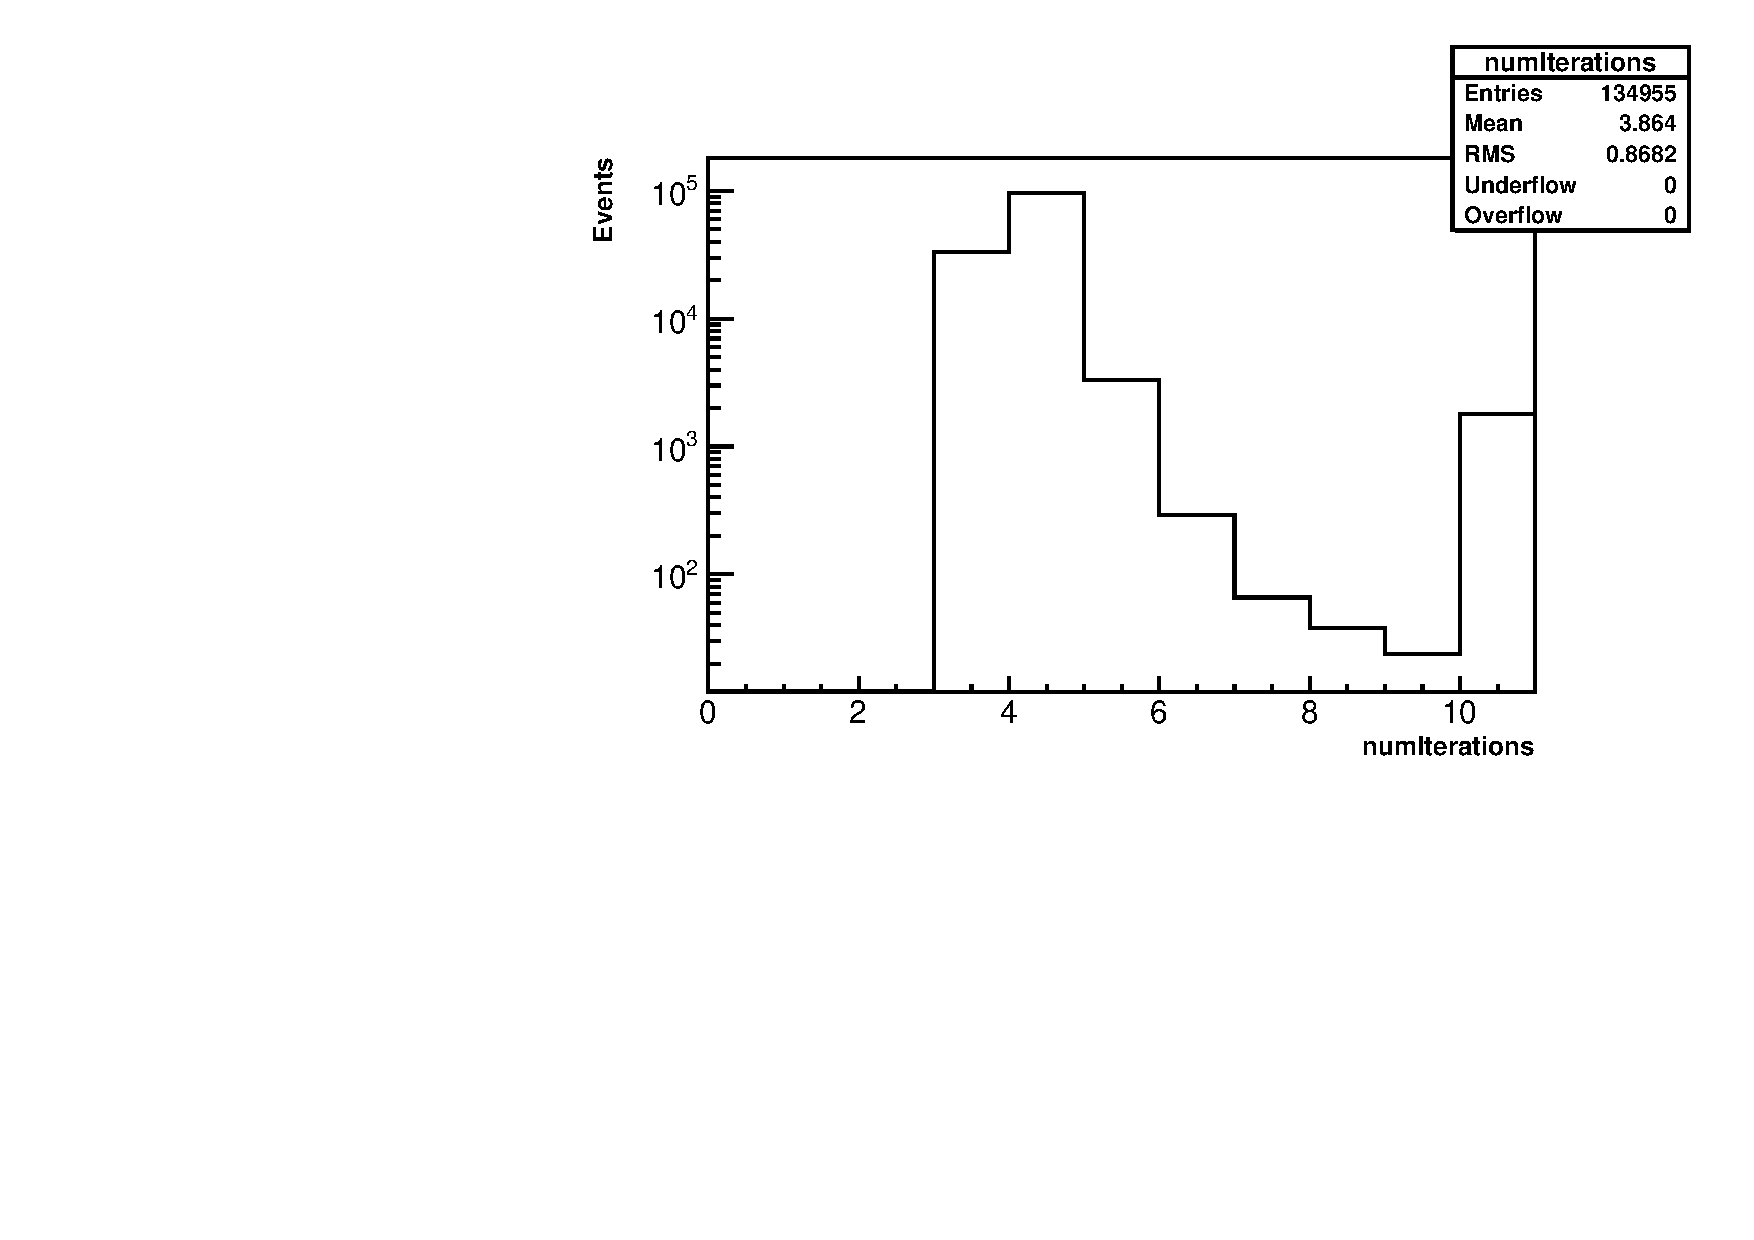
\includegraphics[width=1\textwidth]{numIterationsLog} 
        \caption{Number of iterations log plot. The number of iterations is manually cut off at 10, which is why there is an increase in the last bin and no overflows.}
    \end{subfigure}

    \caption{Number of iterations information.}
\end{figure}



\begin{figure}
    \centering
    \begin{subfigure}[]{0.65\textwidth}
        \centering
        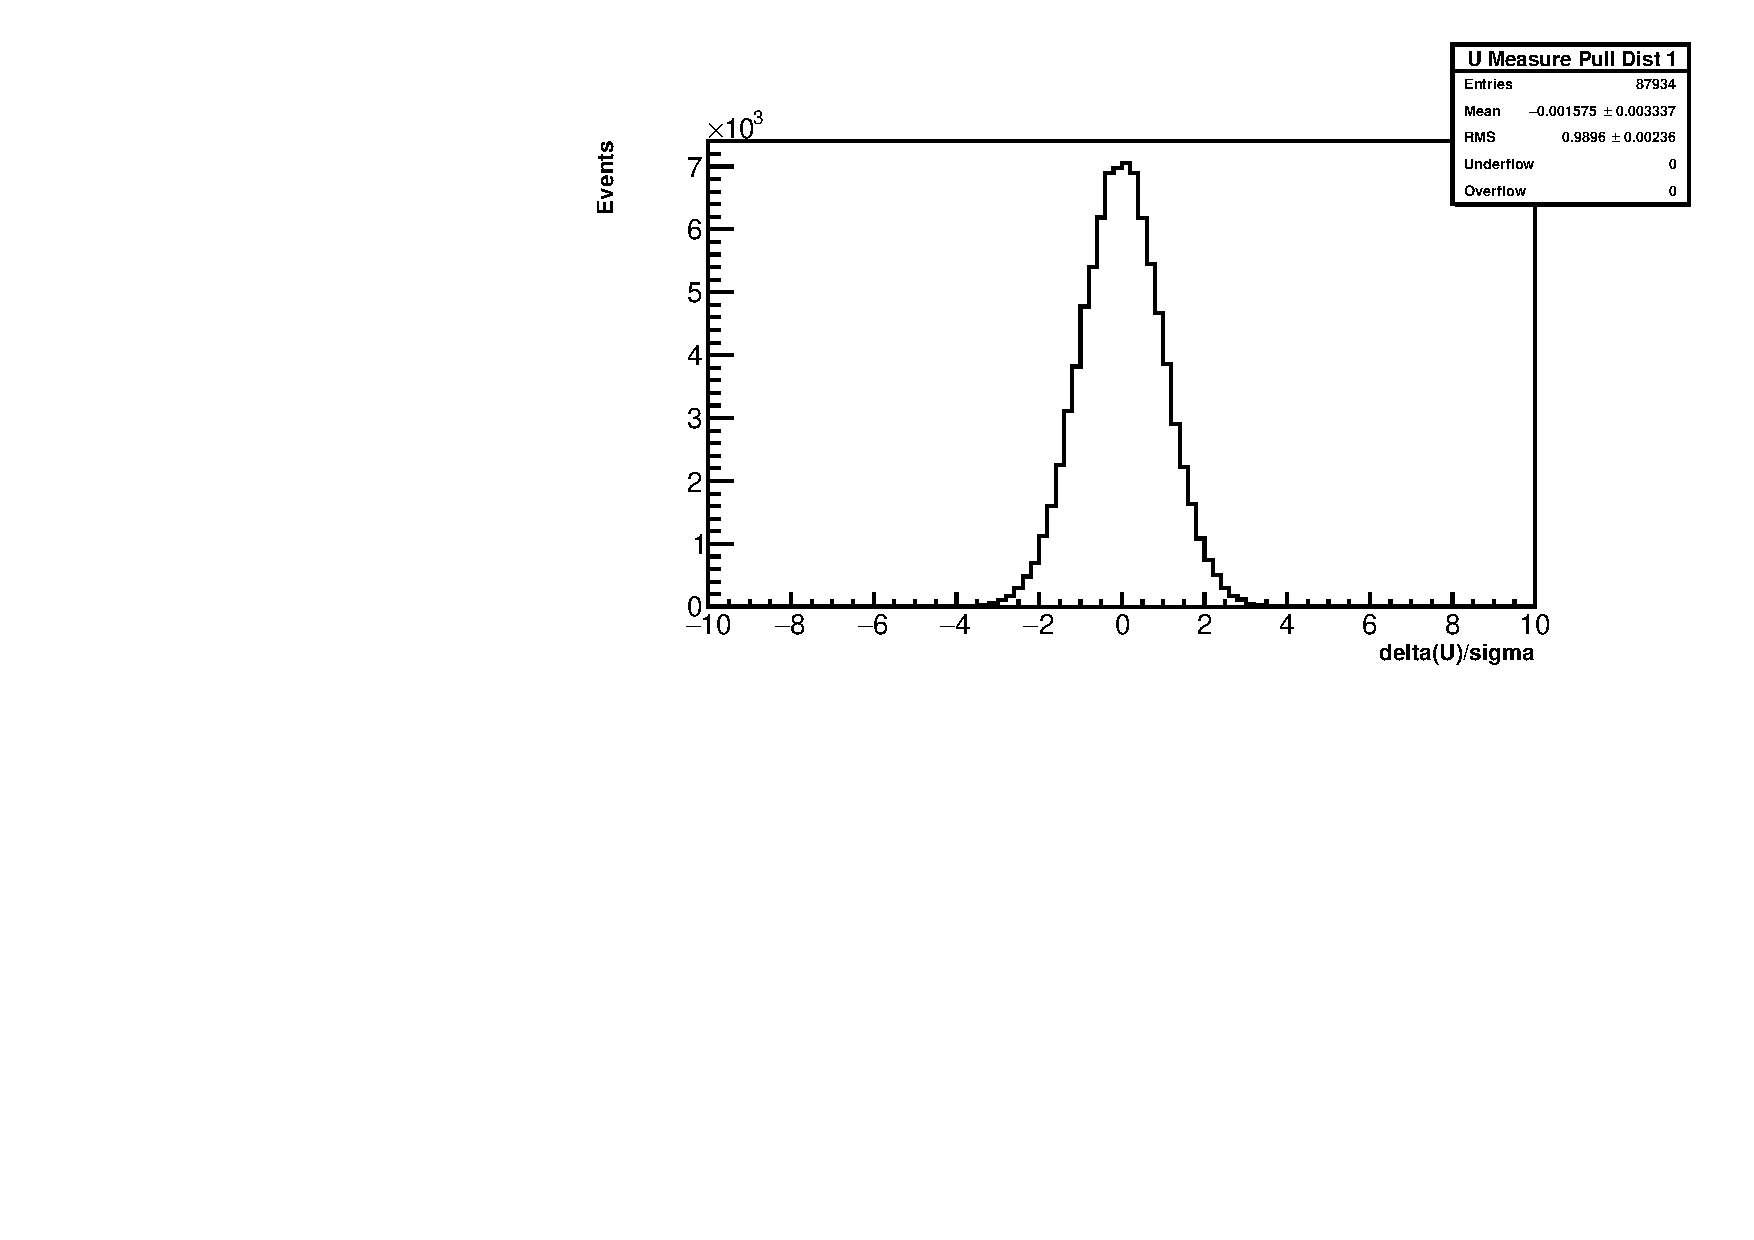
\includegraphics[width=1\textwidth]{UmeasPull} 
        \caption{U measurement pull on plane 1 as given by Equation \ref{eq:measpullmaterial}. It is a unit Gaussian within errors.}
    \end{subfigure}
    
    \begin{subfigure}[]{0.65\textwidth}
        \centering
        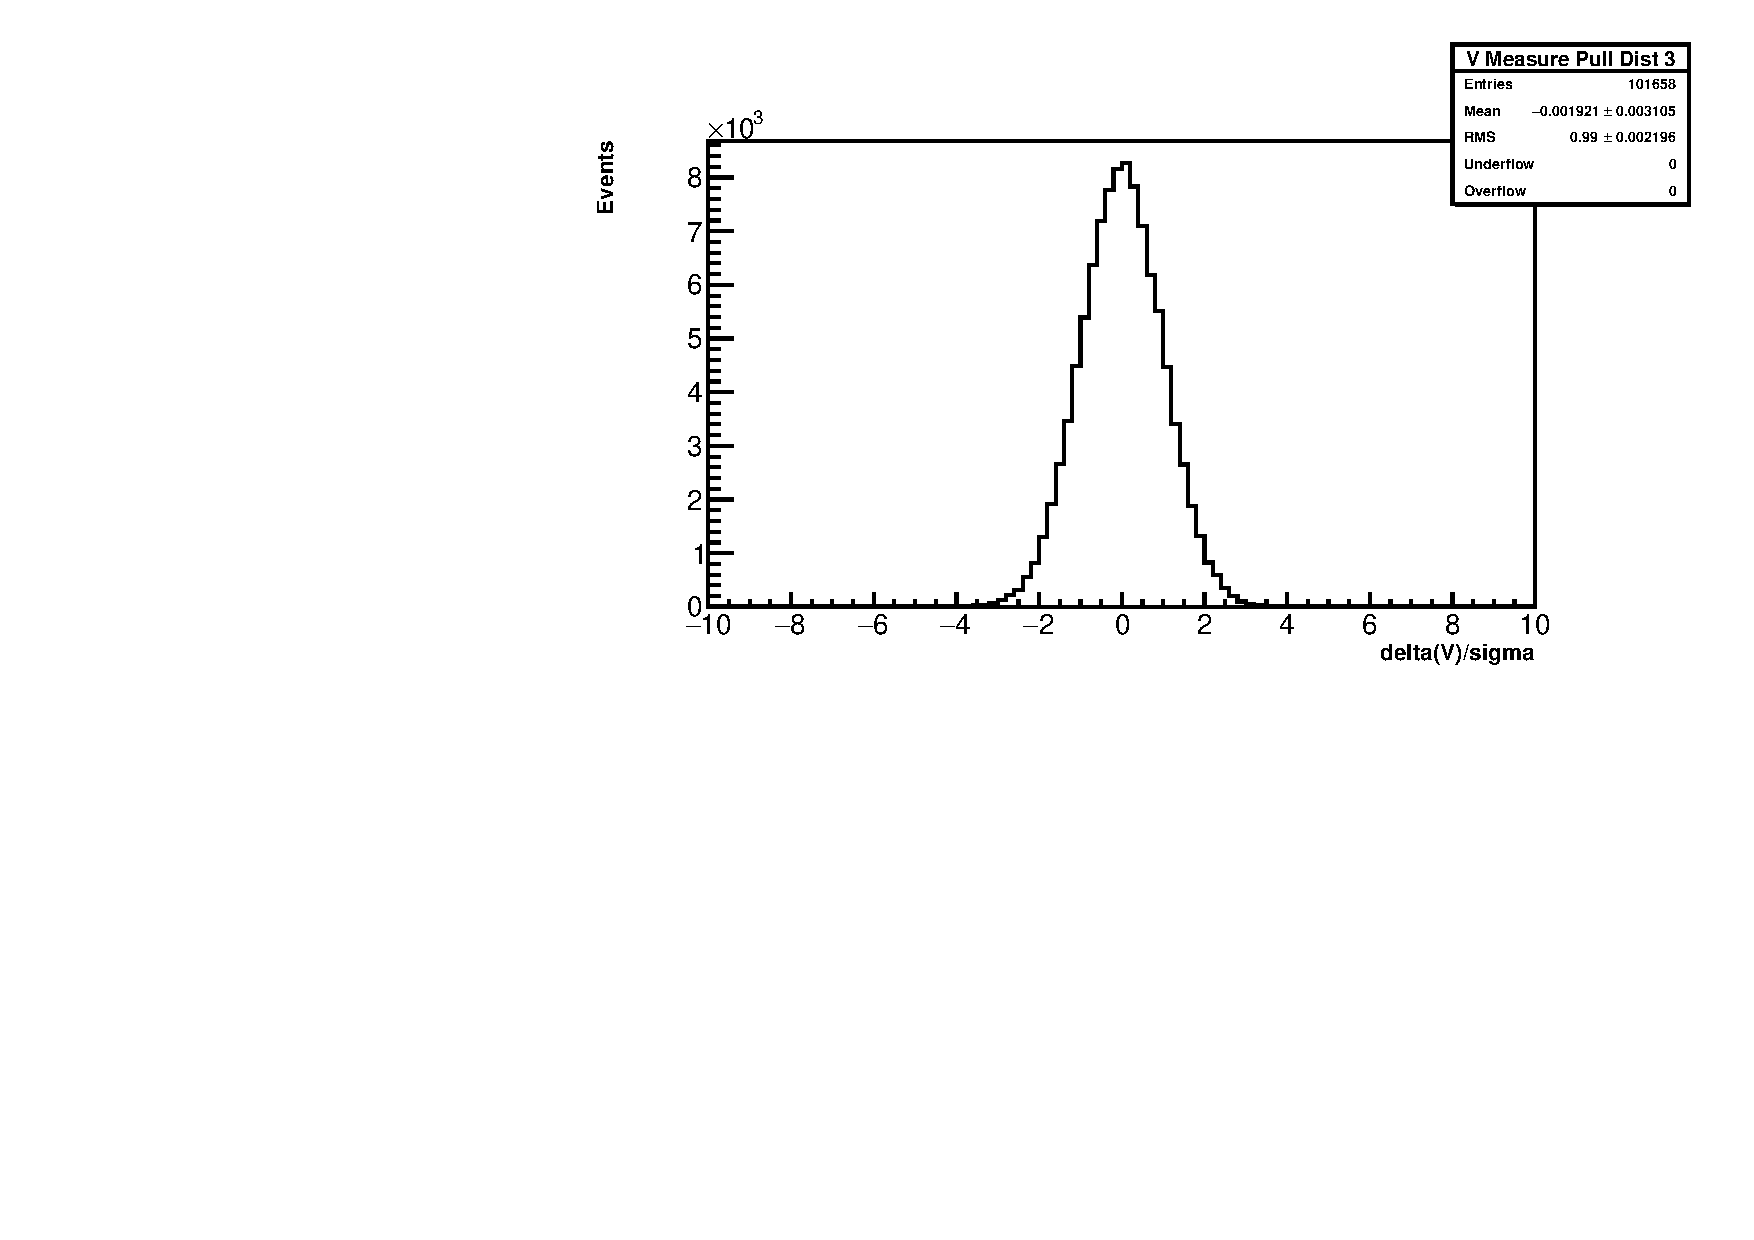
\includegraphics[width=1\textwidth]{VmeasPull} 
        \caption{V measurement pull on plane 3 as given by Equation \ref{eq:measpullmaterial}. It is a unit Gaussian within errors.}
    \end{subfigure}

    \begin{subfigure}[]{0.65\textwidth}
        \centering
        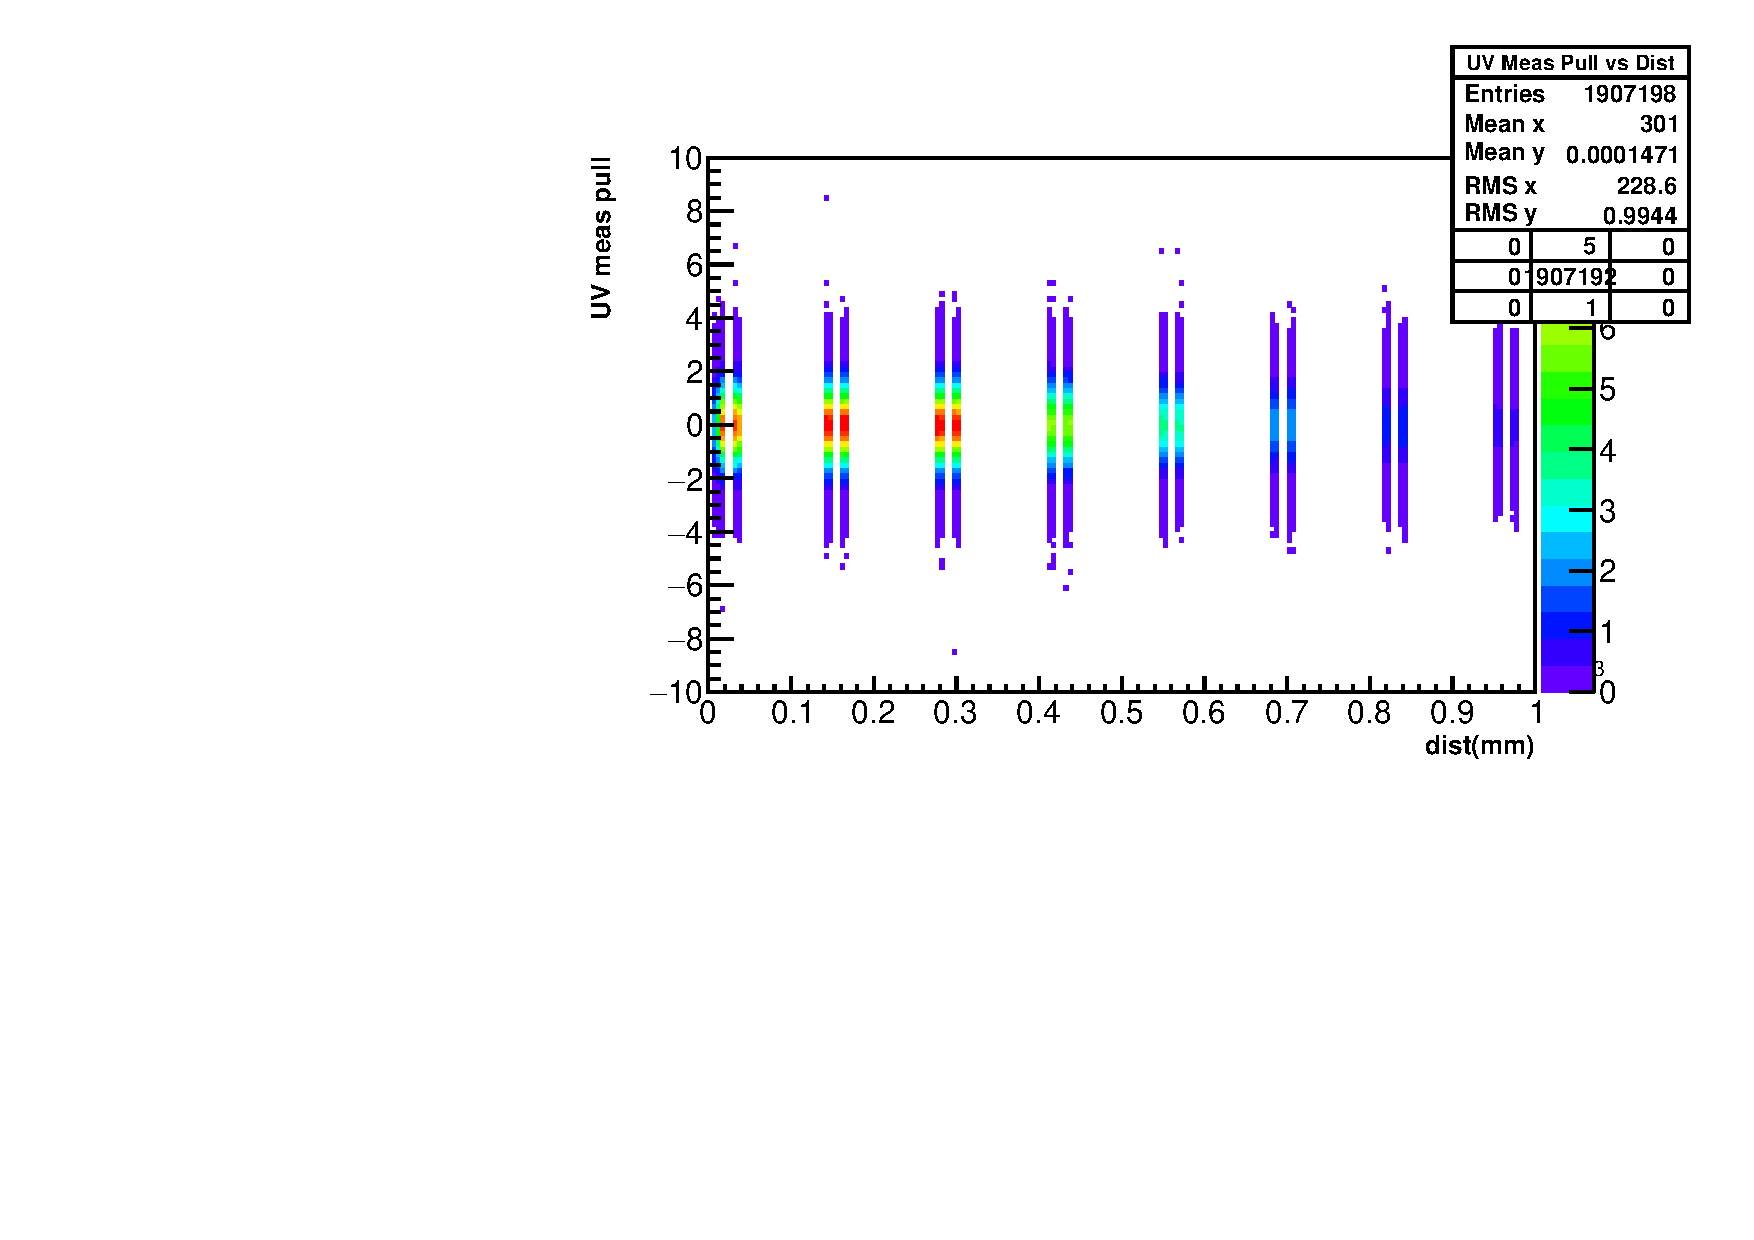
\includegraphics[width=1\textwidth]{UVMeasPullVsDist} 
        \caption{U and V measurement pulls as a function of track distance from fitting start point, or ``0'' plane. The RMS drops slightly as a function of distance, indicated imperfectly attuned errors.}
    \end{subfigure}

    \caption{Measurement pull plots, useful for track fitting on data validation.}
\end{figure}



\begin{figure}
    \centering
    \begin{subfigure}[]{0.65\textwidth}
        \centering
        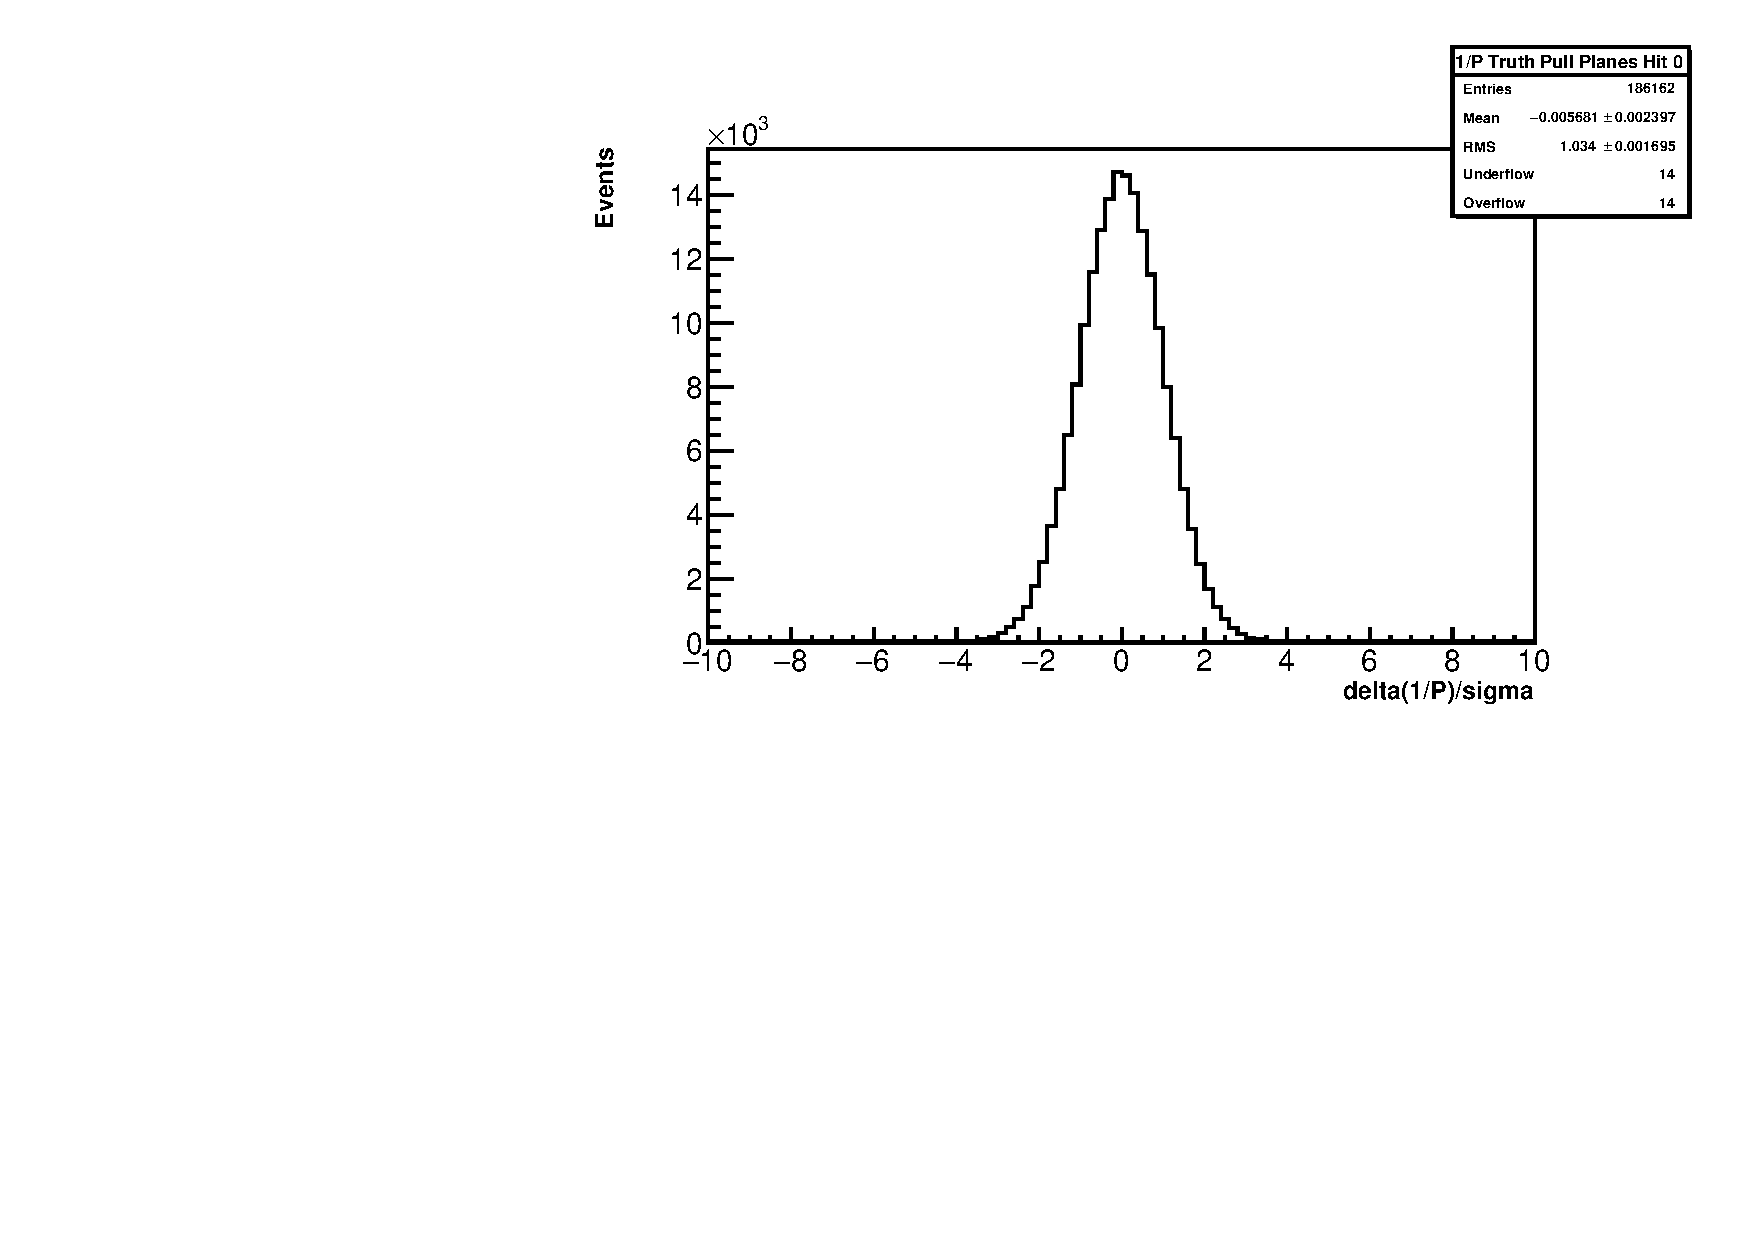
\includegraphics[width=1\textwidth]{1Ppull} 
        \caption{1/P truth pull on plane 0 for all tracks. Very close to a unit Gaussian showing the tracking is working correctly.}
    \end{subfigure}
    
    \begin{subfigure}[]{0.65\textwidth}
        \centering
        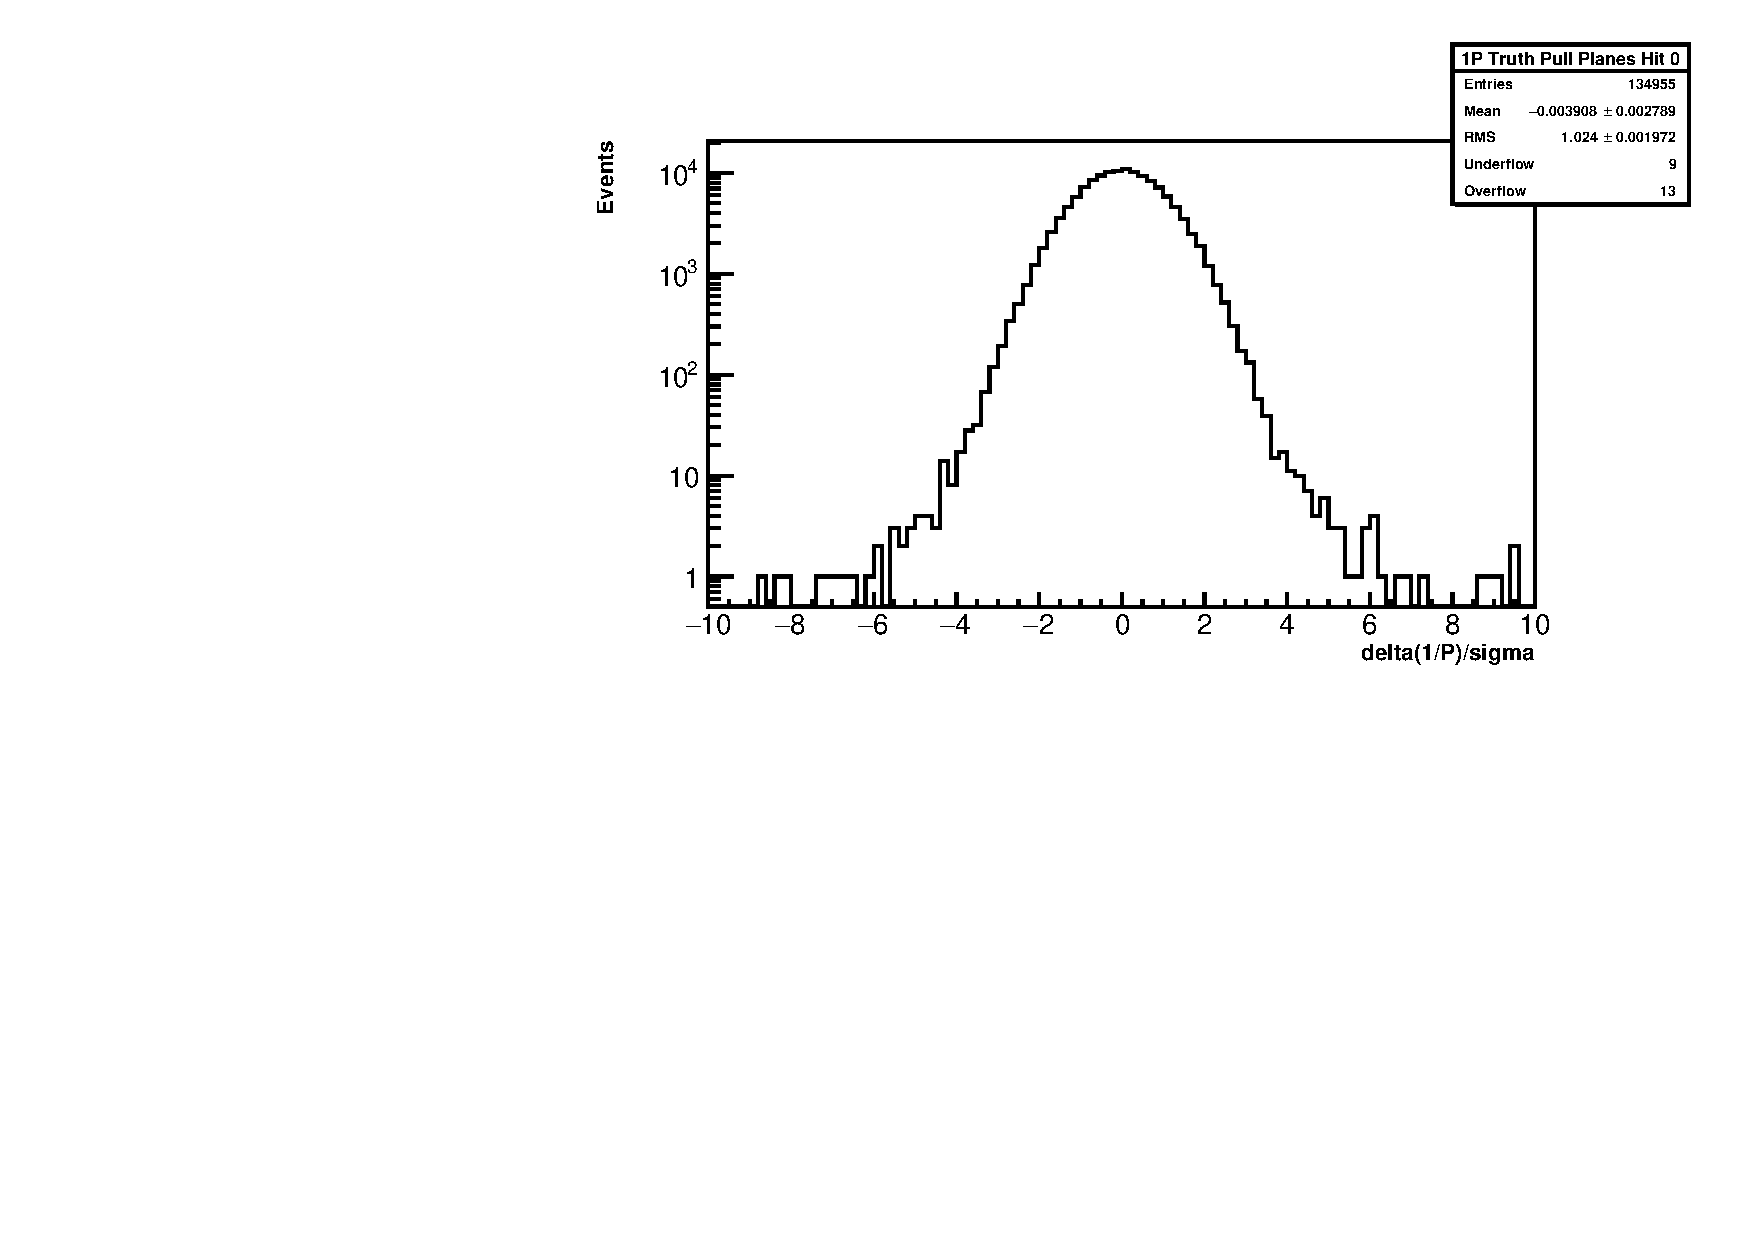
\includegraphics[width=1\textwidth]{1PpullLog} 
        \caption{1/P truth pull on plane 0 for all tracks, log plot. Poor events can be seen as the distribution spreads out more towards the edges, with some under and overflows.}
    \end{subfigure}

    \begin{subfigure}[]{0.65\textwidth}
        \centering
        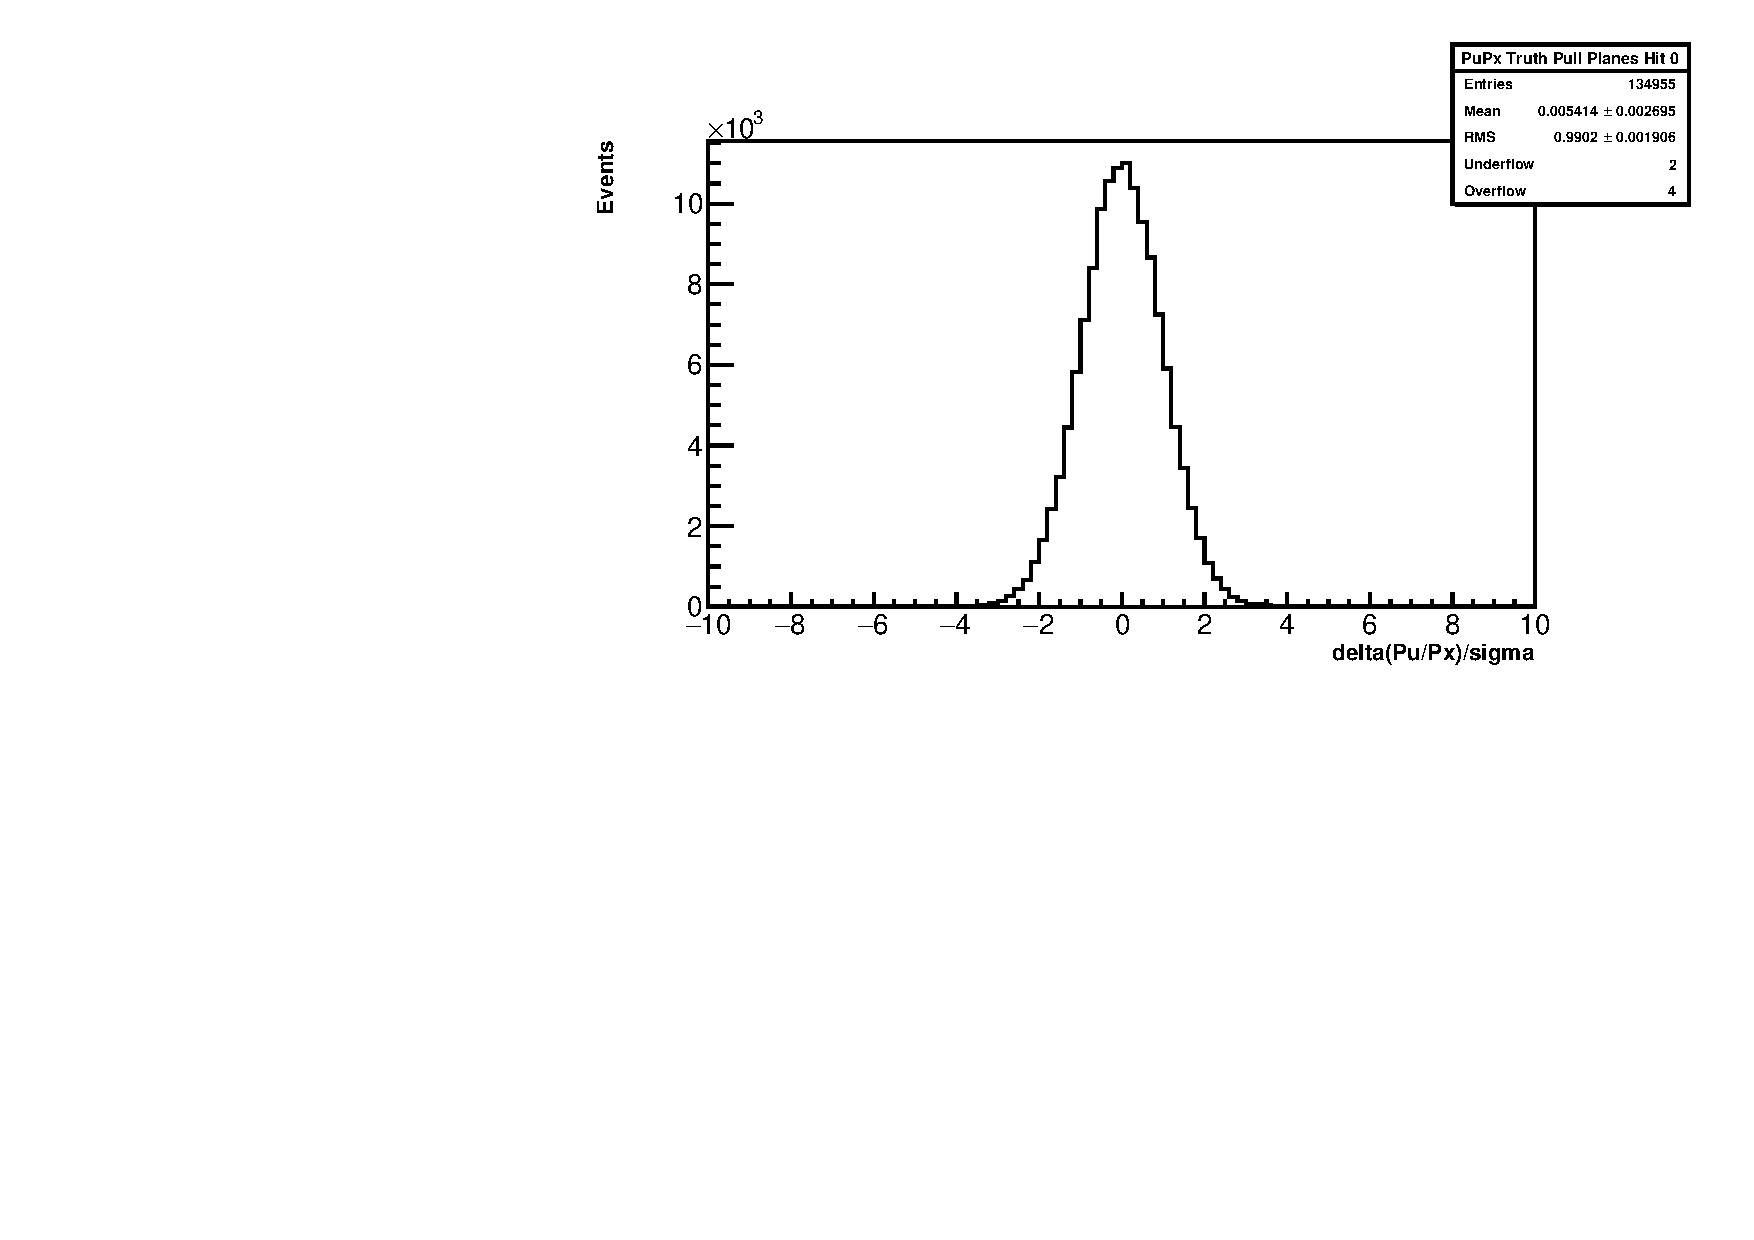
\includegraphics[width=1\textwidth]{PuPxpull} 
        \caption{Pu/Px truth pull on plane 0 for all tracks. Very close to a unit Gaussian showing the tracking is working correctly.}
    \end{subfigure}

    \caption{Truth pulls on plane 0 for all tracks.}
\end{figure}



\begin{figure}
    \centering
    \begin{subfigure}[]{0.65\textwidth}
        \centering
        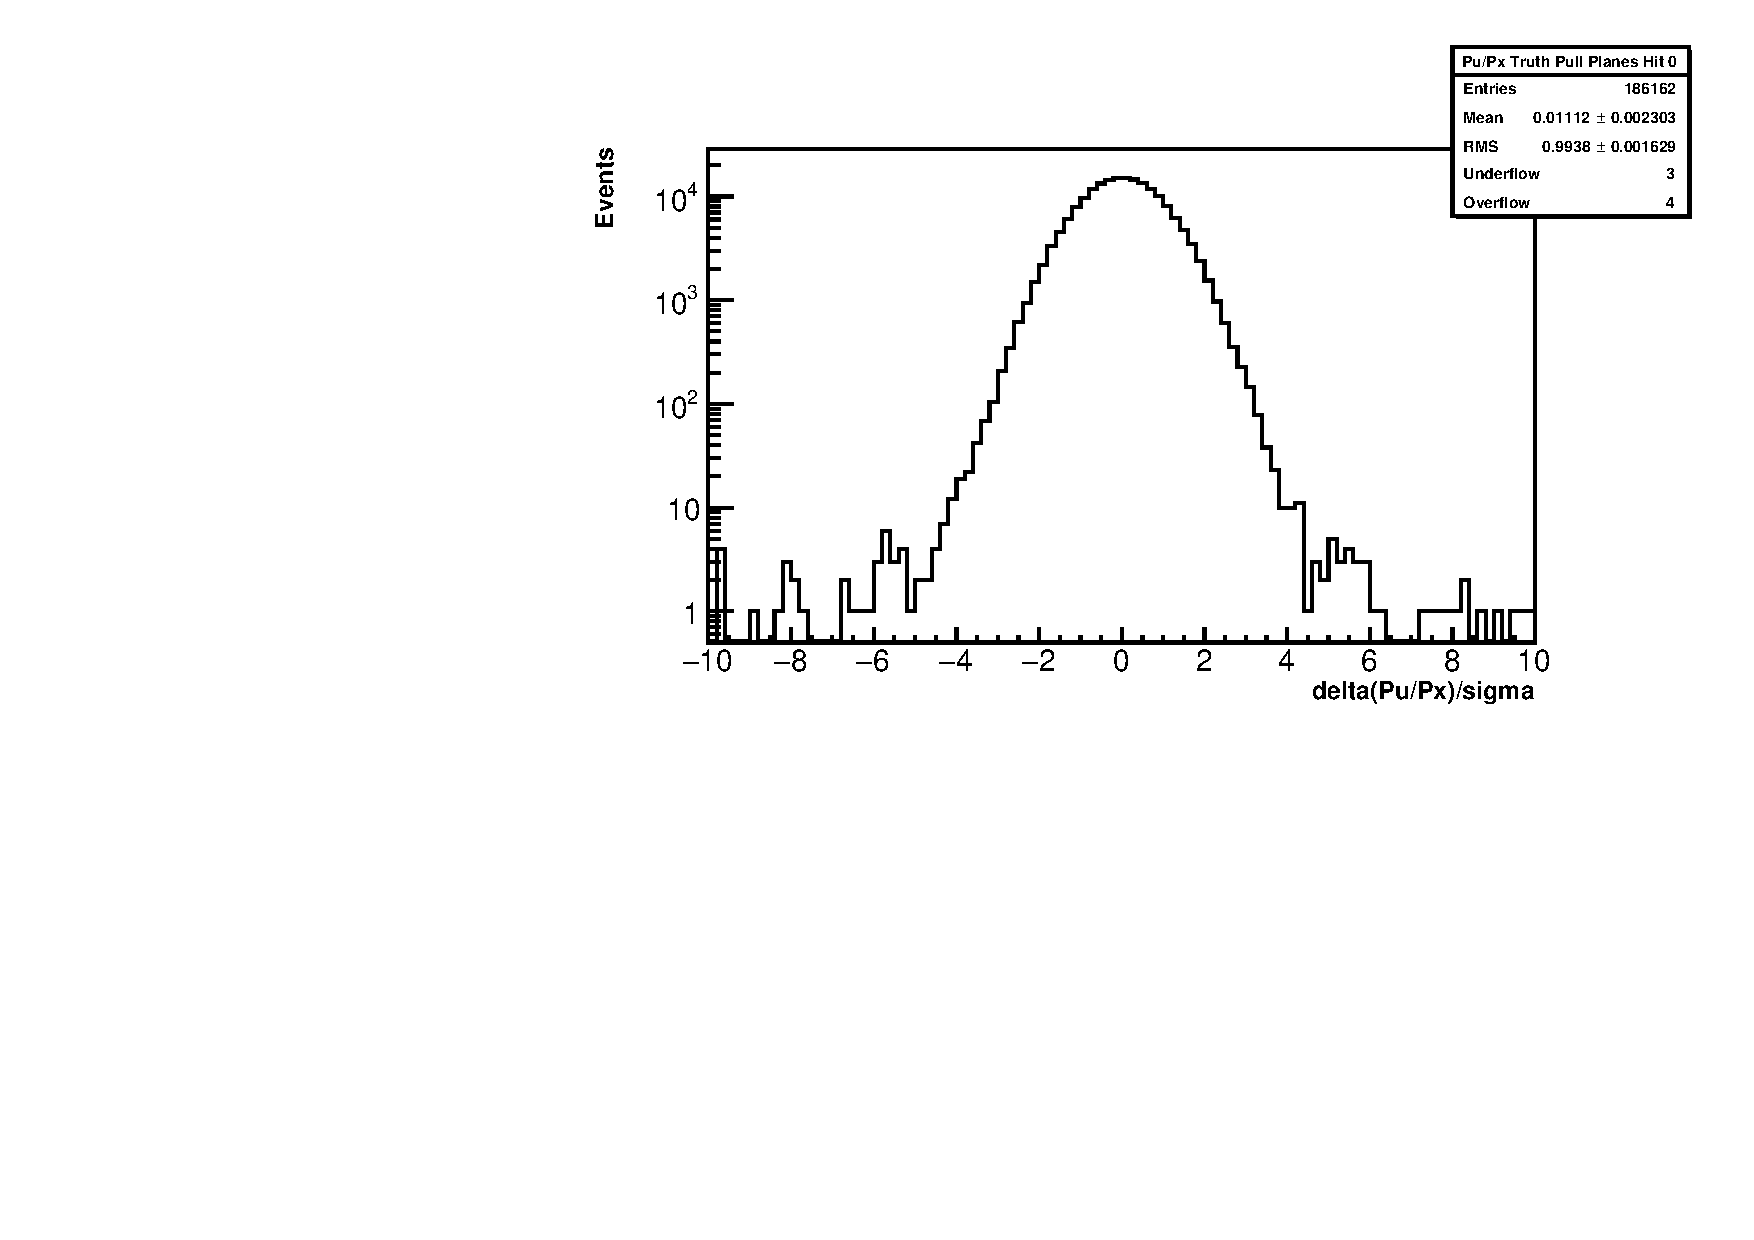
\includegraphics[width=1\textwidth]{PuPxpullLog} 
        \caption{Pu/Px truth pull on plane 0 for all tracks, log plot. Poor events can be seen as the distribution spreads out more towards the edges, with some under and overflows.}
    \end{subfigure}
    
    \begin{subfigure}[]{0.65\textwidth}
        \centering
        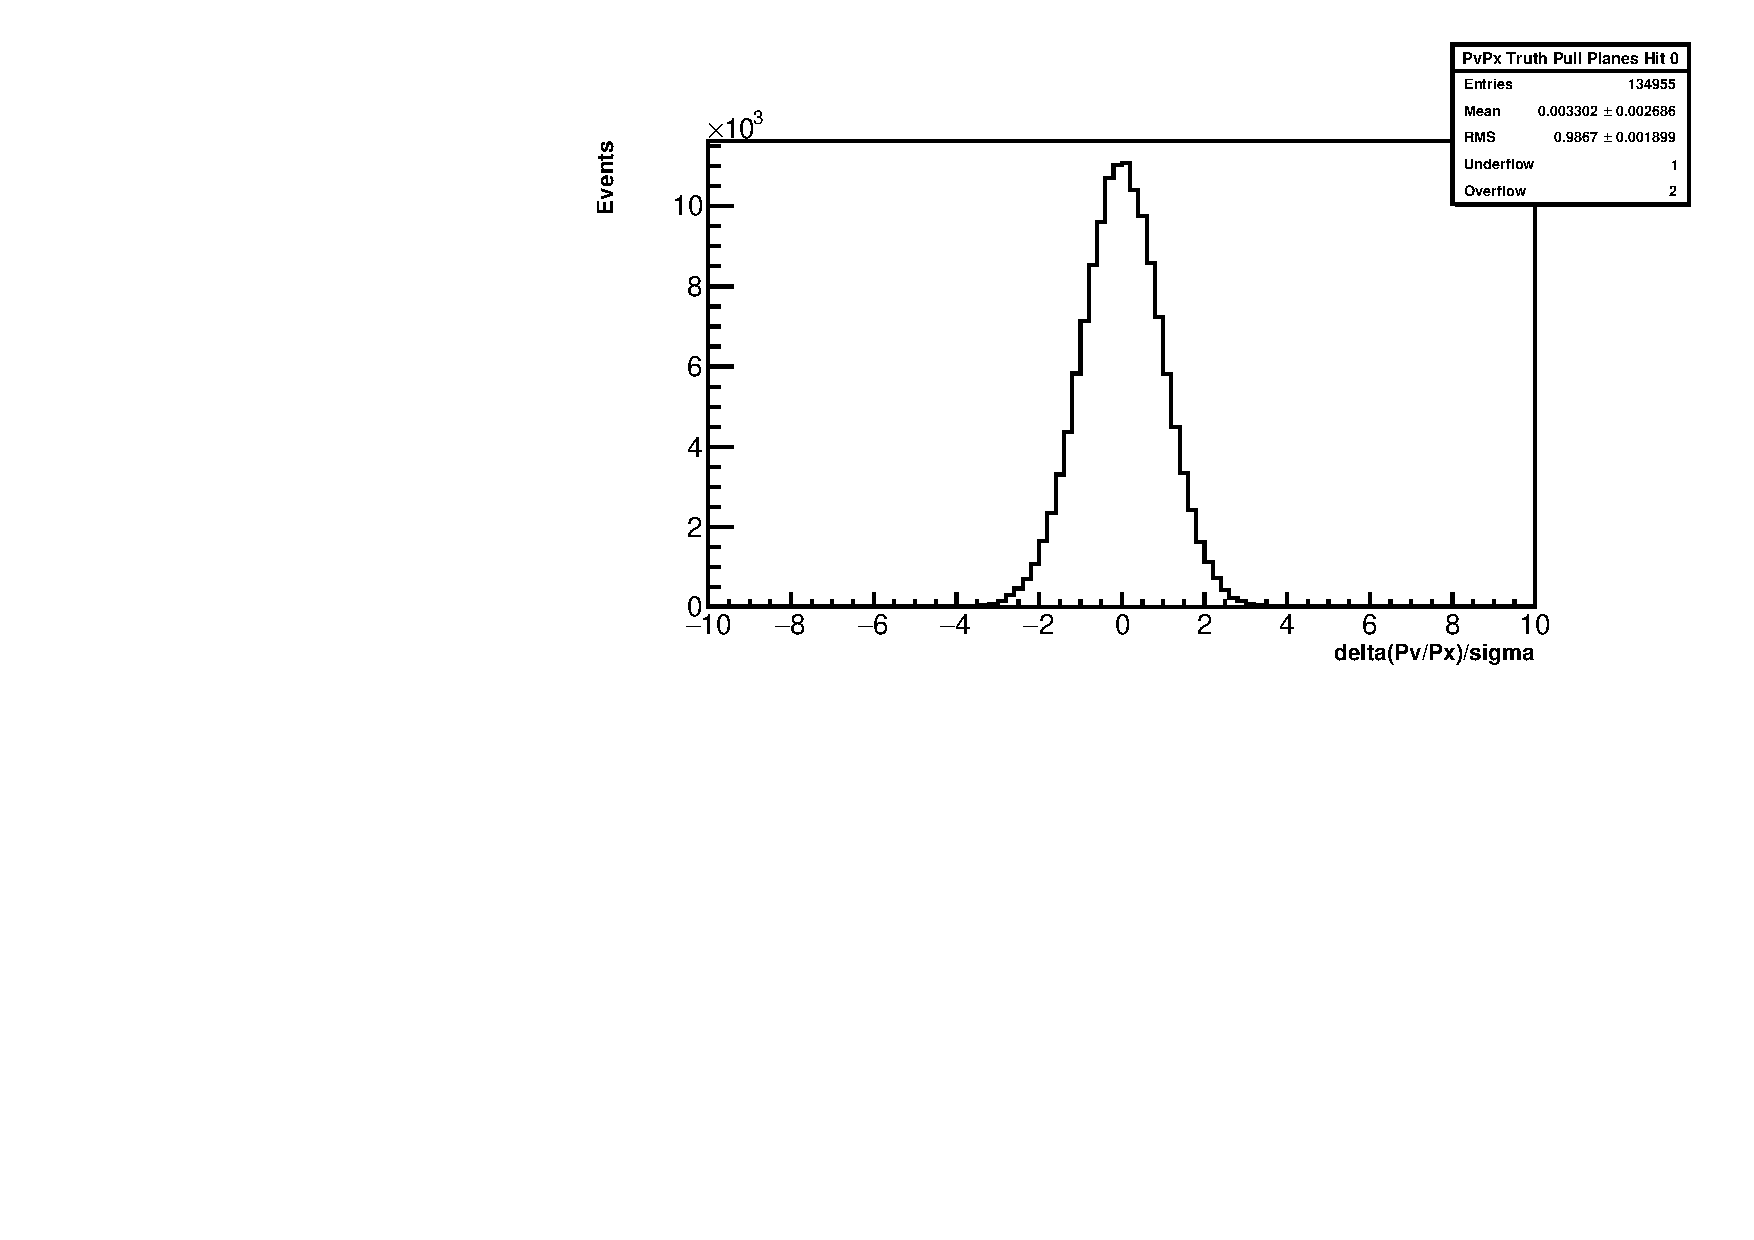
\includegraphics[width=1\textwidth]{PvPxpull} 
        \caption{Pv/Px truth pull on plane 0 for all tracks. Very close to a unit Gaussian showing the tracking is working correctly.}
    \end{subfigure}

    \begin{subfigure}[]{0.65\textwidth}
        \centering
        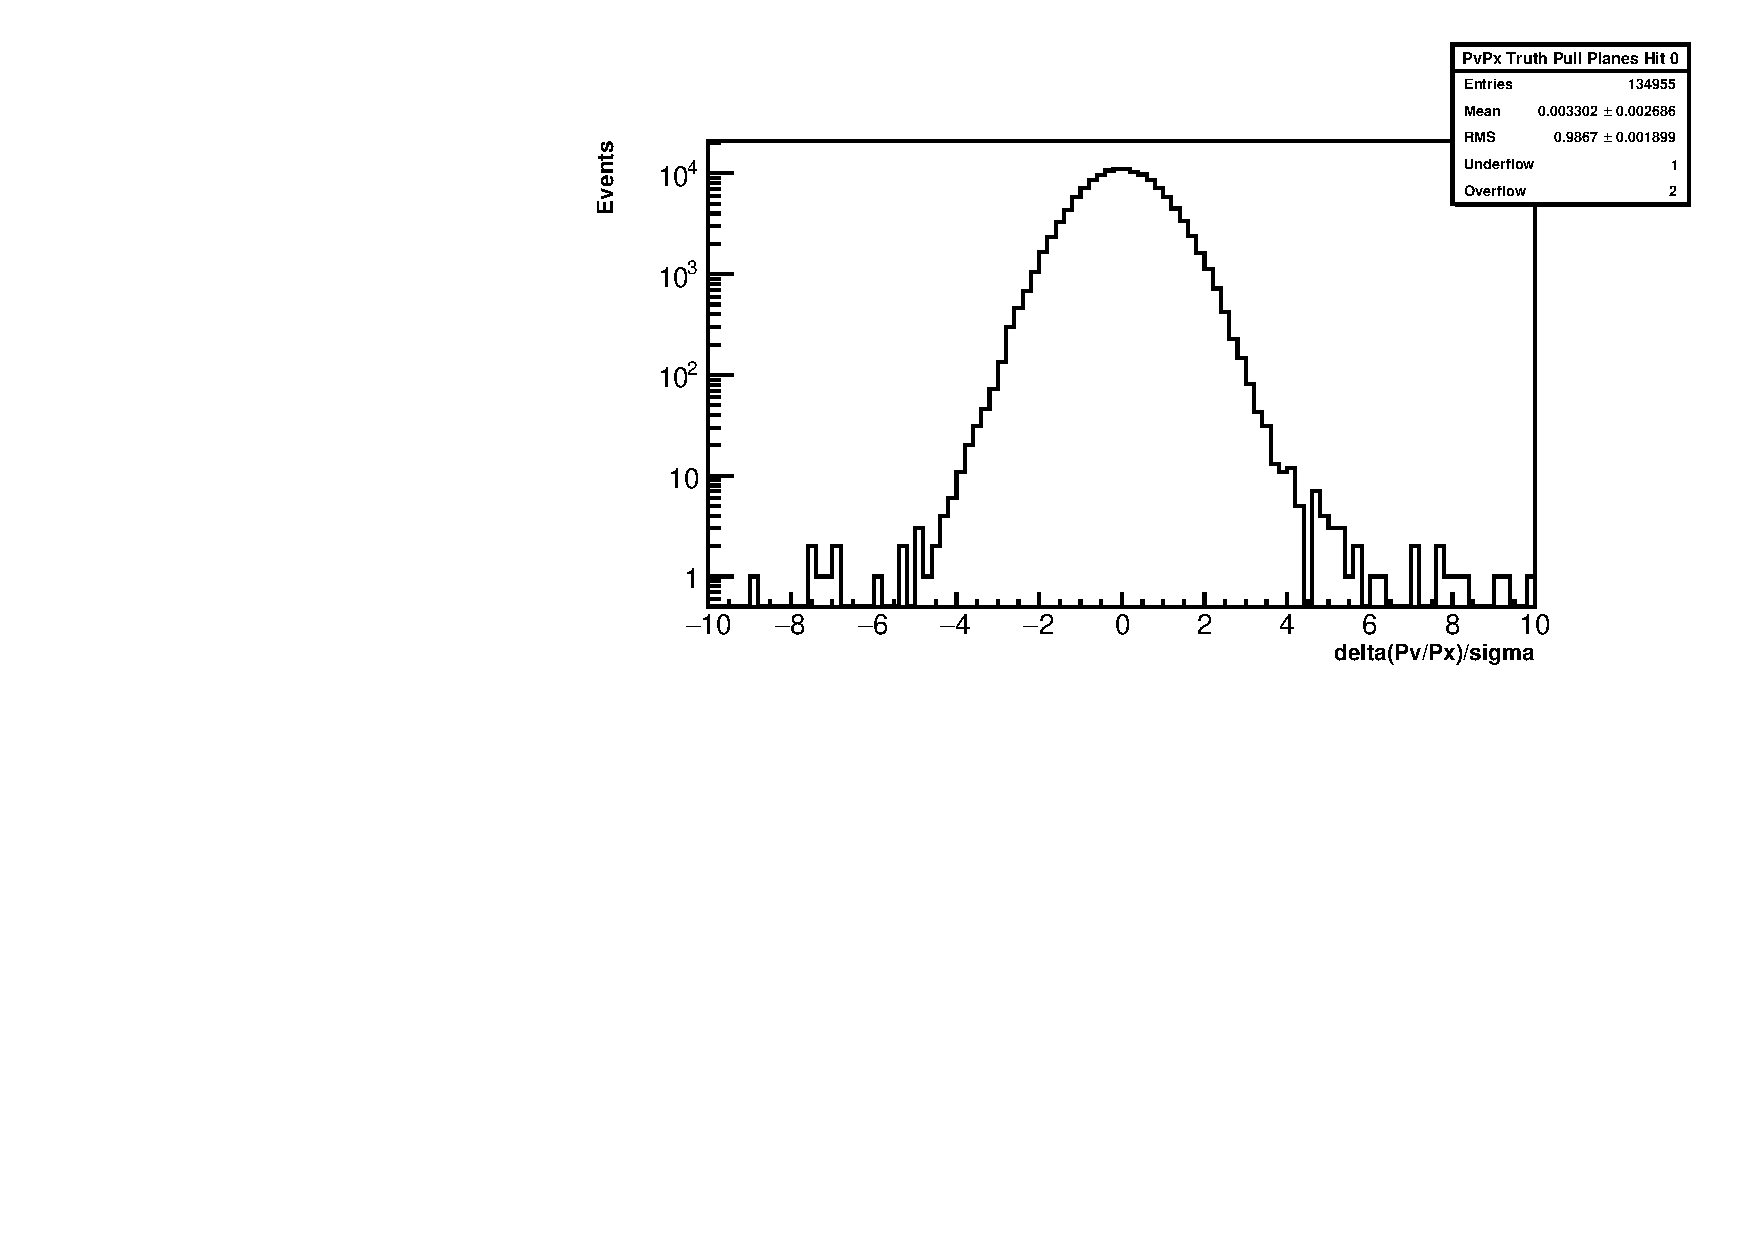
\includegraphics[width=1\textwidth]{PvPxpullLog} 
        \caption{Pv/Px truth pull on plane 0 for all tracks, log plot. Poor events can be seen as the distribution spreads out more towards the edges, with some under and overflows.}
    \end{subfigure}

    \caption{Truth pulls on plane 0 for all tracks.}
\end{figure}



\begin{figure}
    \centering
    \begin{subfigure}[]{0.8\textwidth}
        \centering
        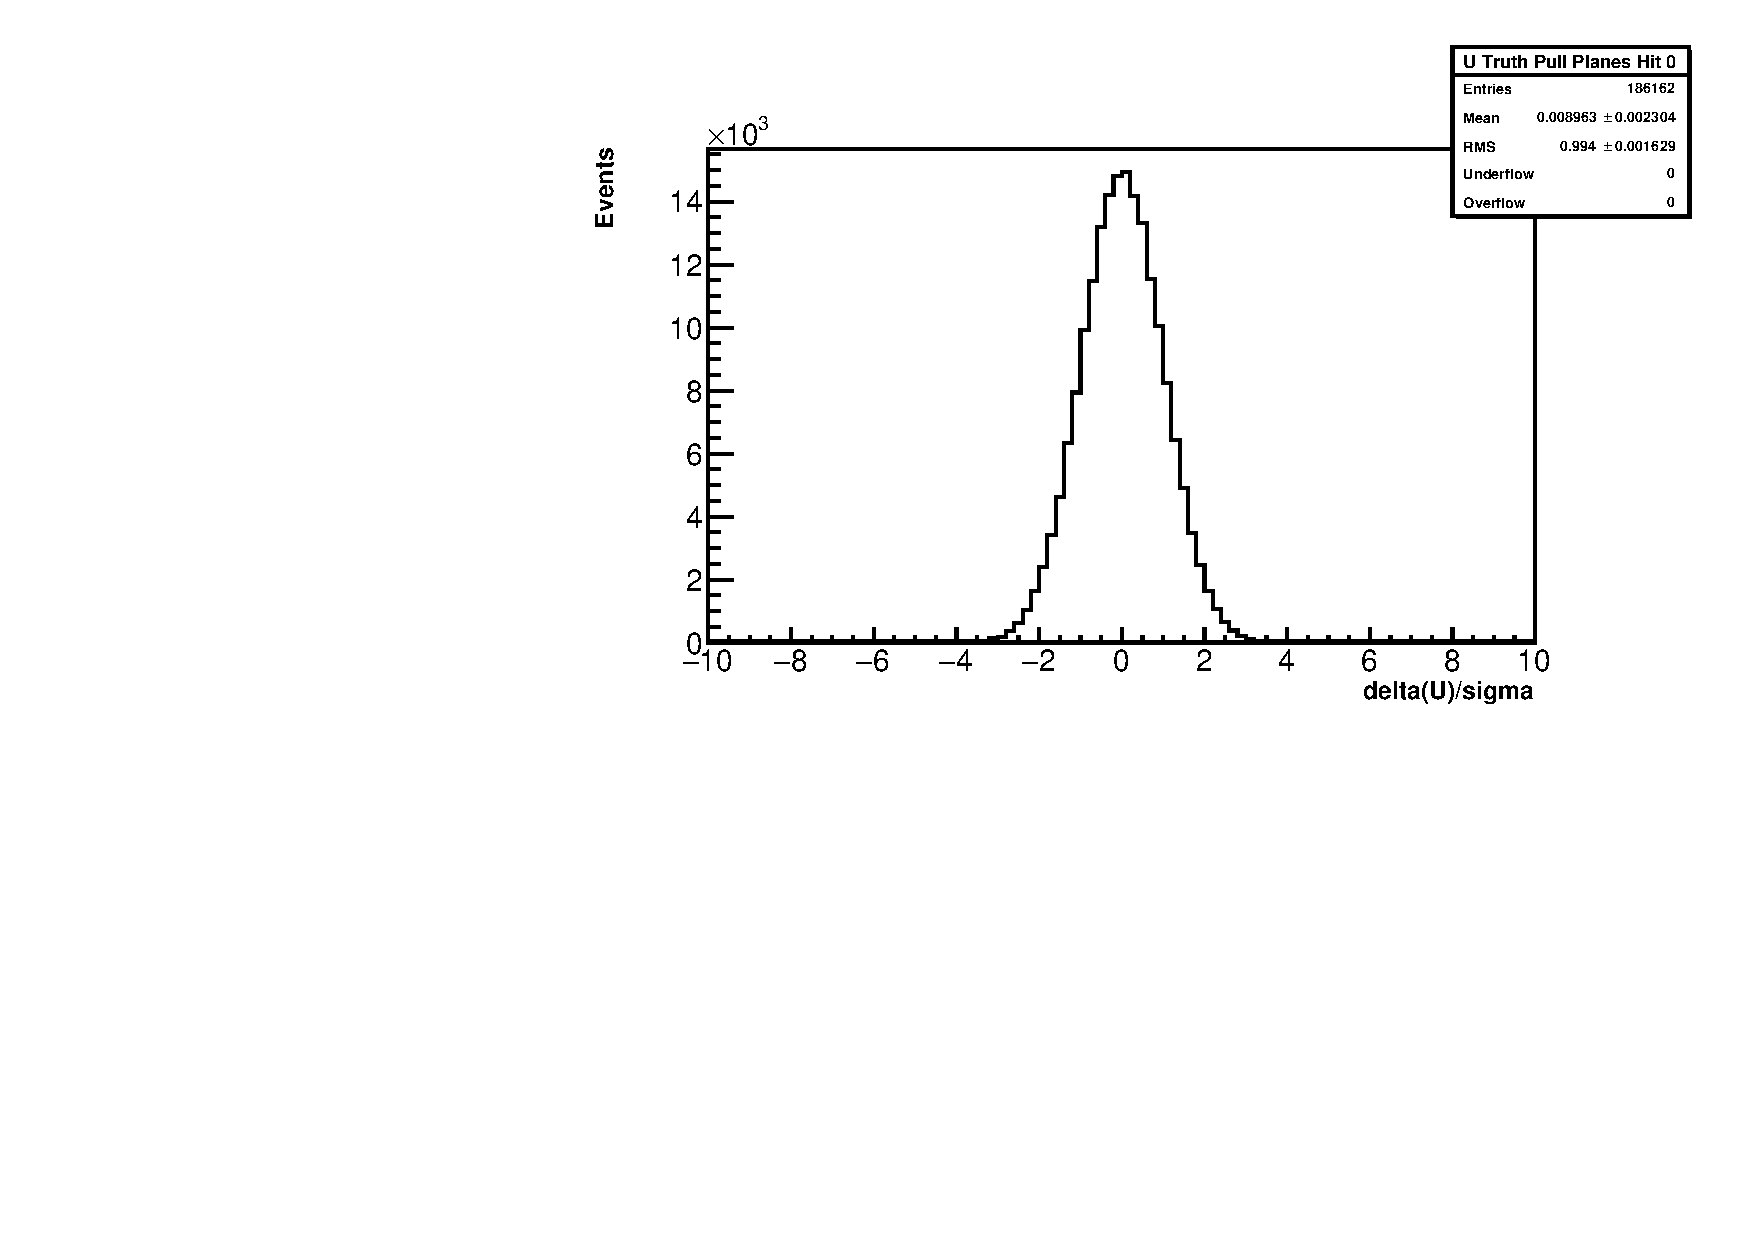
\includegraphics[width=1\textwidth]{Upull} 
        \caption{U truth pull on plane 0 for all tracks. Very close to a unit Gaussian showing the tracking is working correctly.}
    \end{subfigure}
    
    \begin{subfigure}[]{0.8\textwidth}
        \centering
        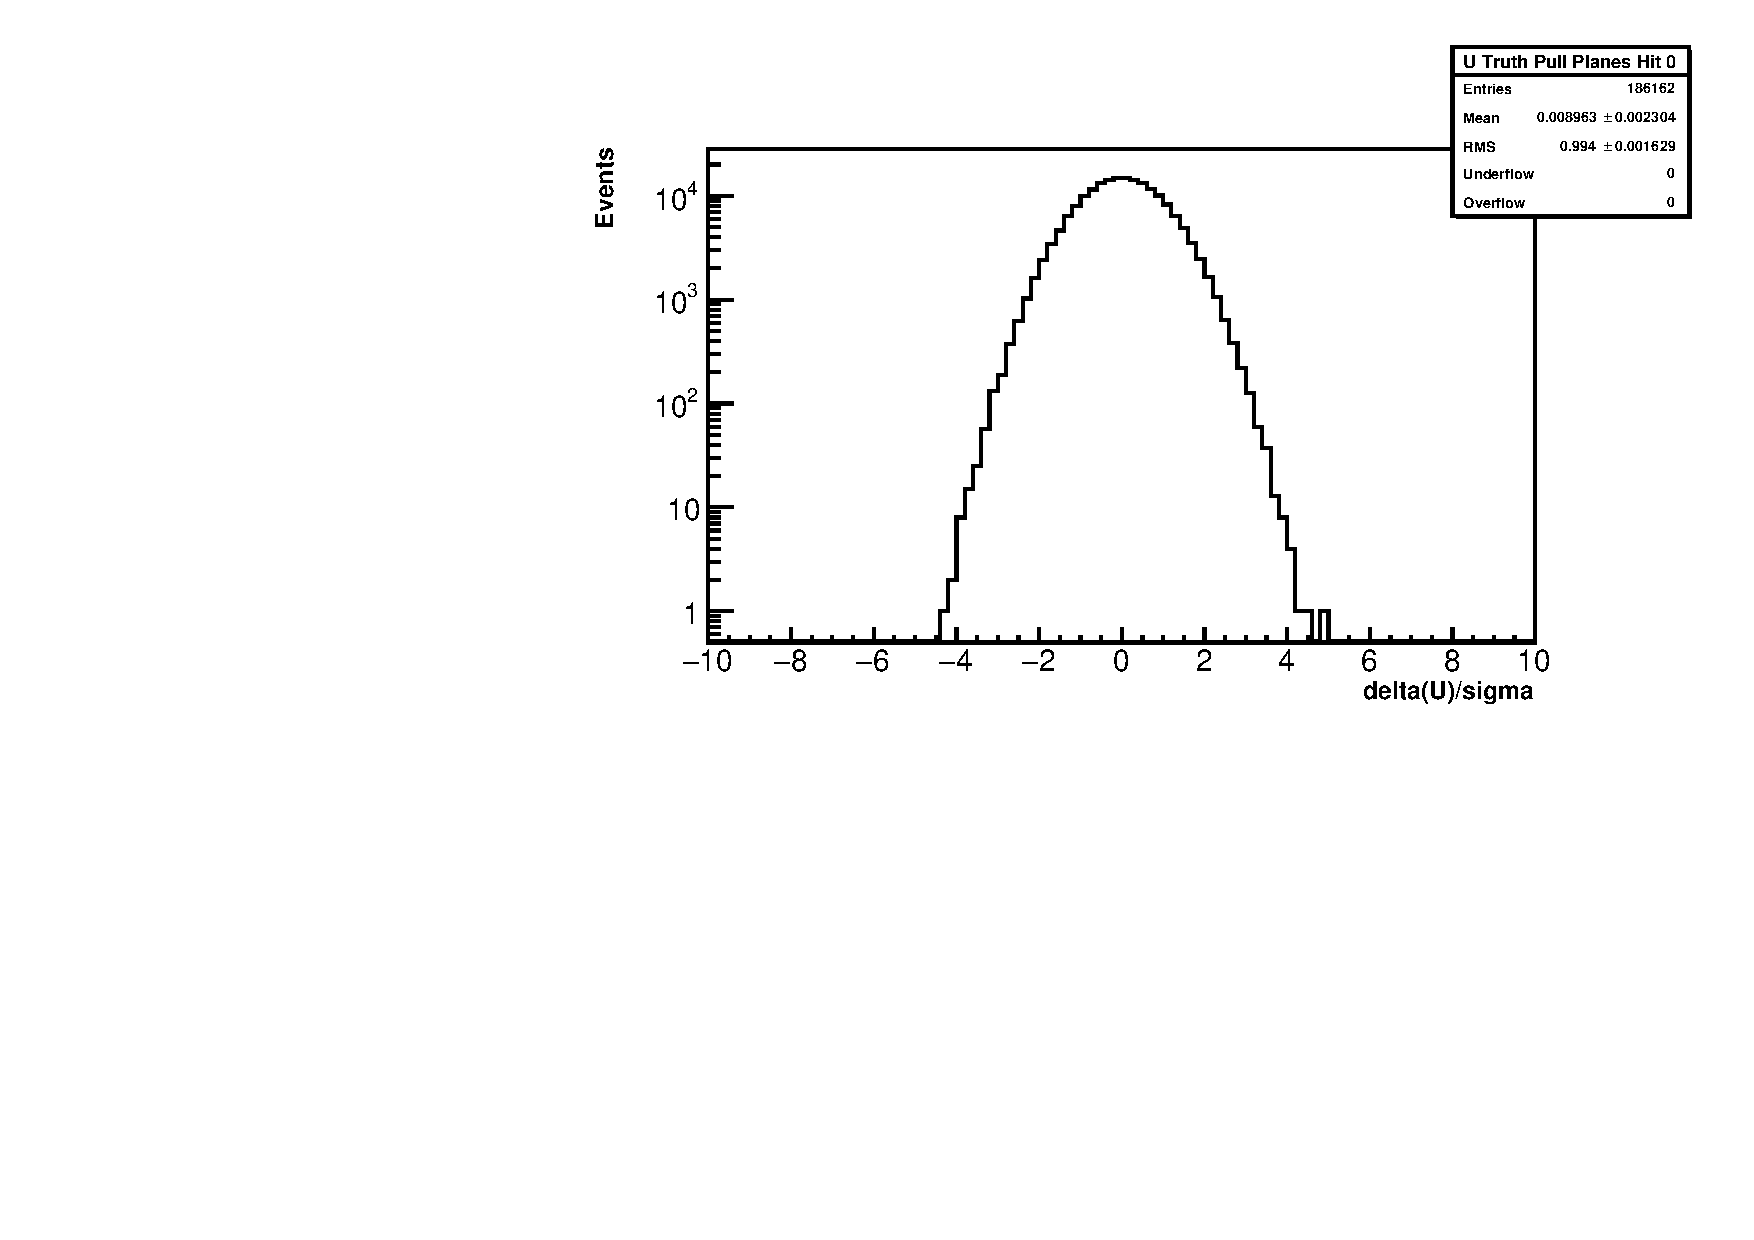
\includegraphics[width=1\textwidth]{UpullLog} 
        \caption{U truth pull on plane 0 for all tracks, log plot. Poor events can be seen as the distribution spreads out more towards the edges, with some under and overflows.}
    \end{subfigure}

    \caption{Number of iterations information.}
\end{figure}

\begin{figure}
    \centering
    \begin{subfigure}[]{0.8\textwidth}
        \centering
        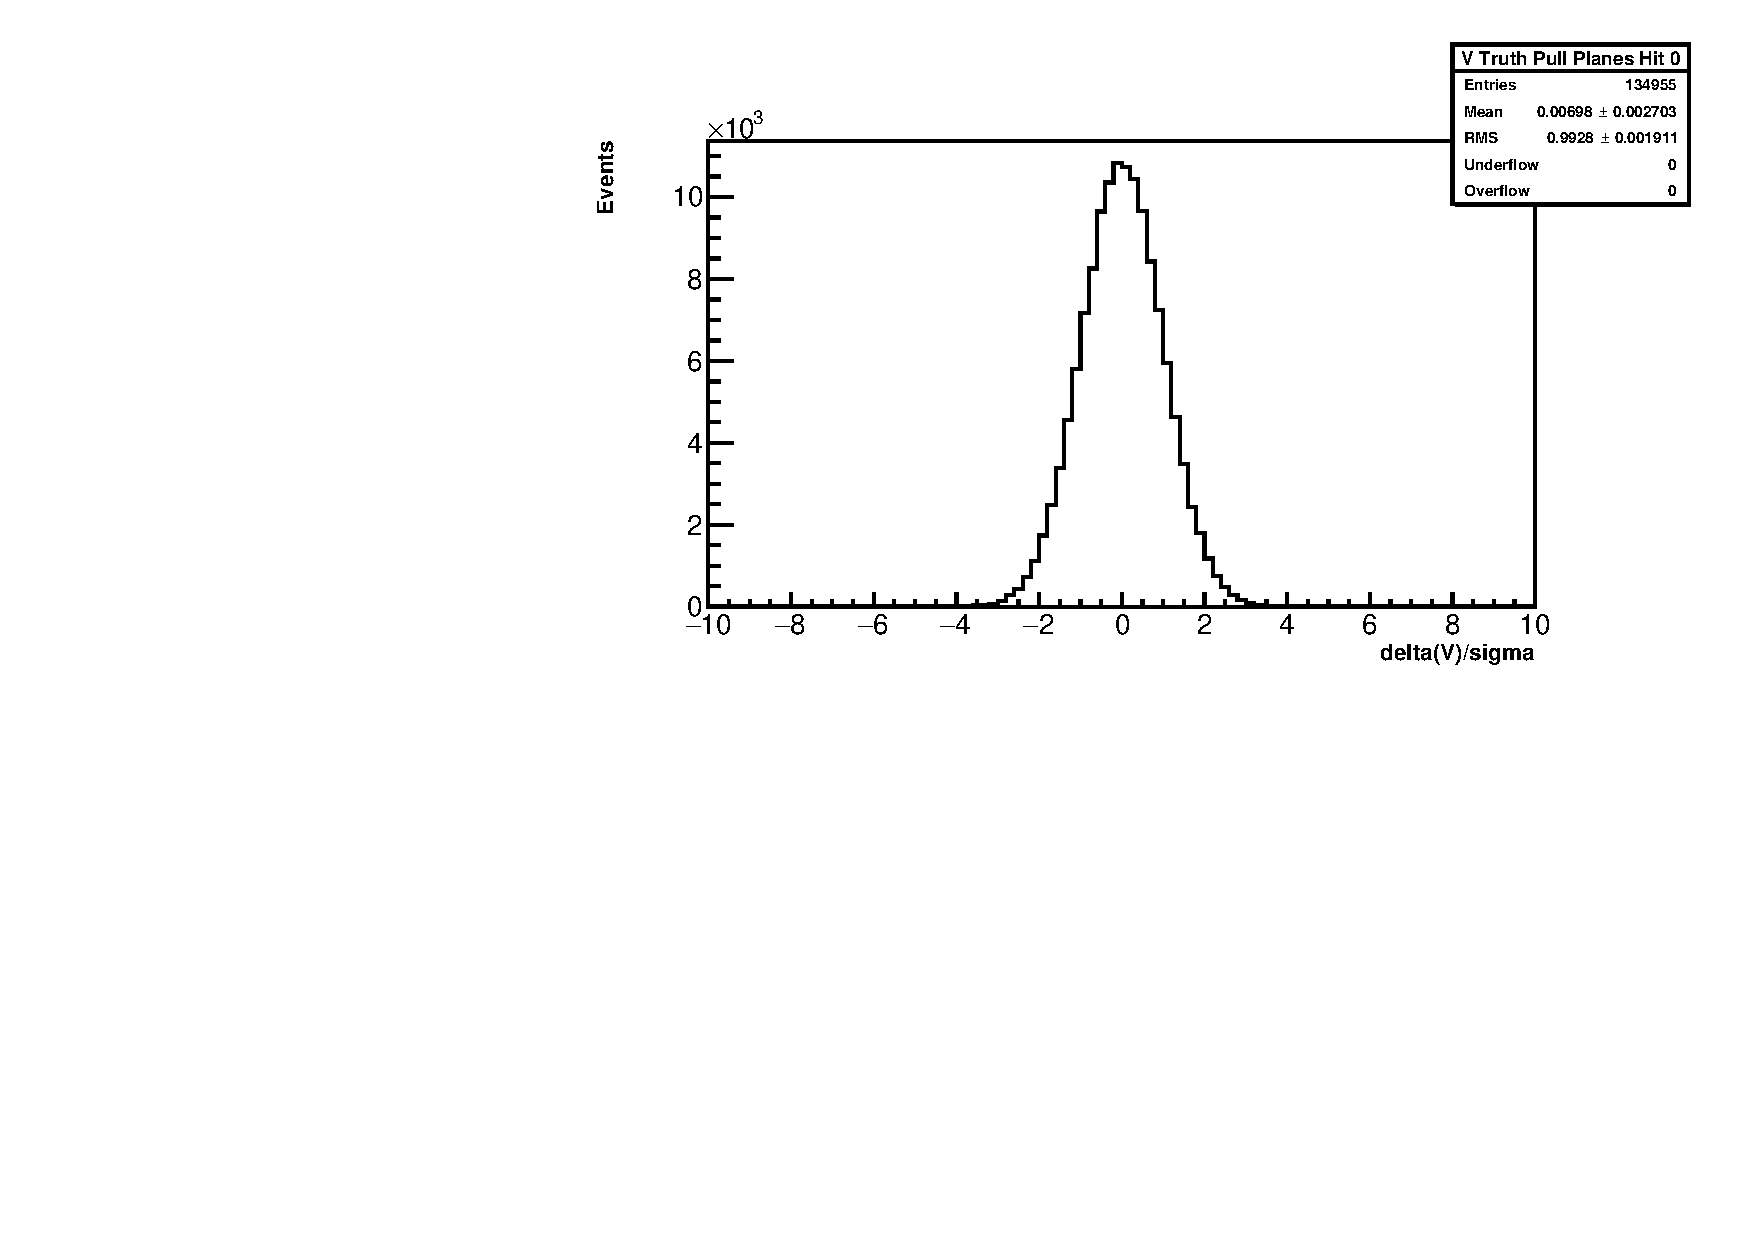
\includegraphics[width=1\textwidth]{Vpull} 
        \caption{V truth pull on plane 0 for all tracks. Very close to a unit Gaussian showing the tracking is working correctly.}
    \end{subfigure}
    
    \begin{subfigure}[]{0.8\textwidth}
        \centering
        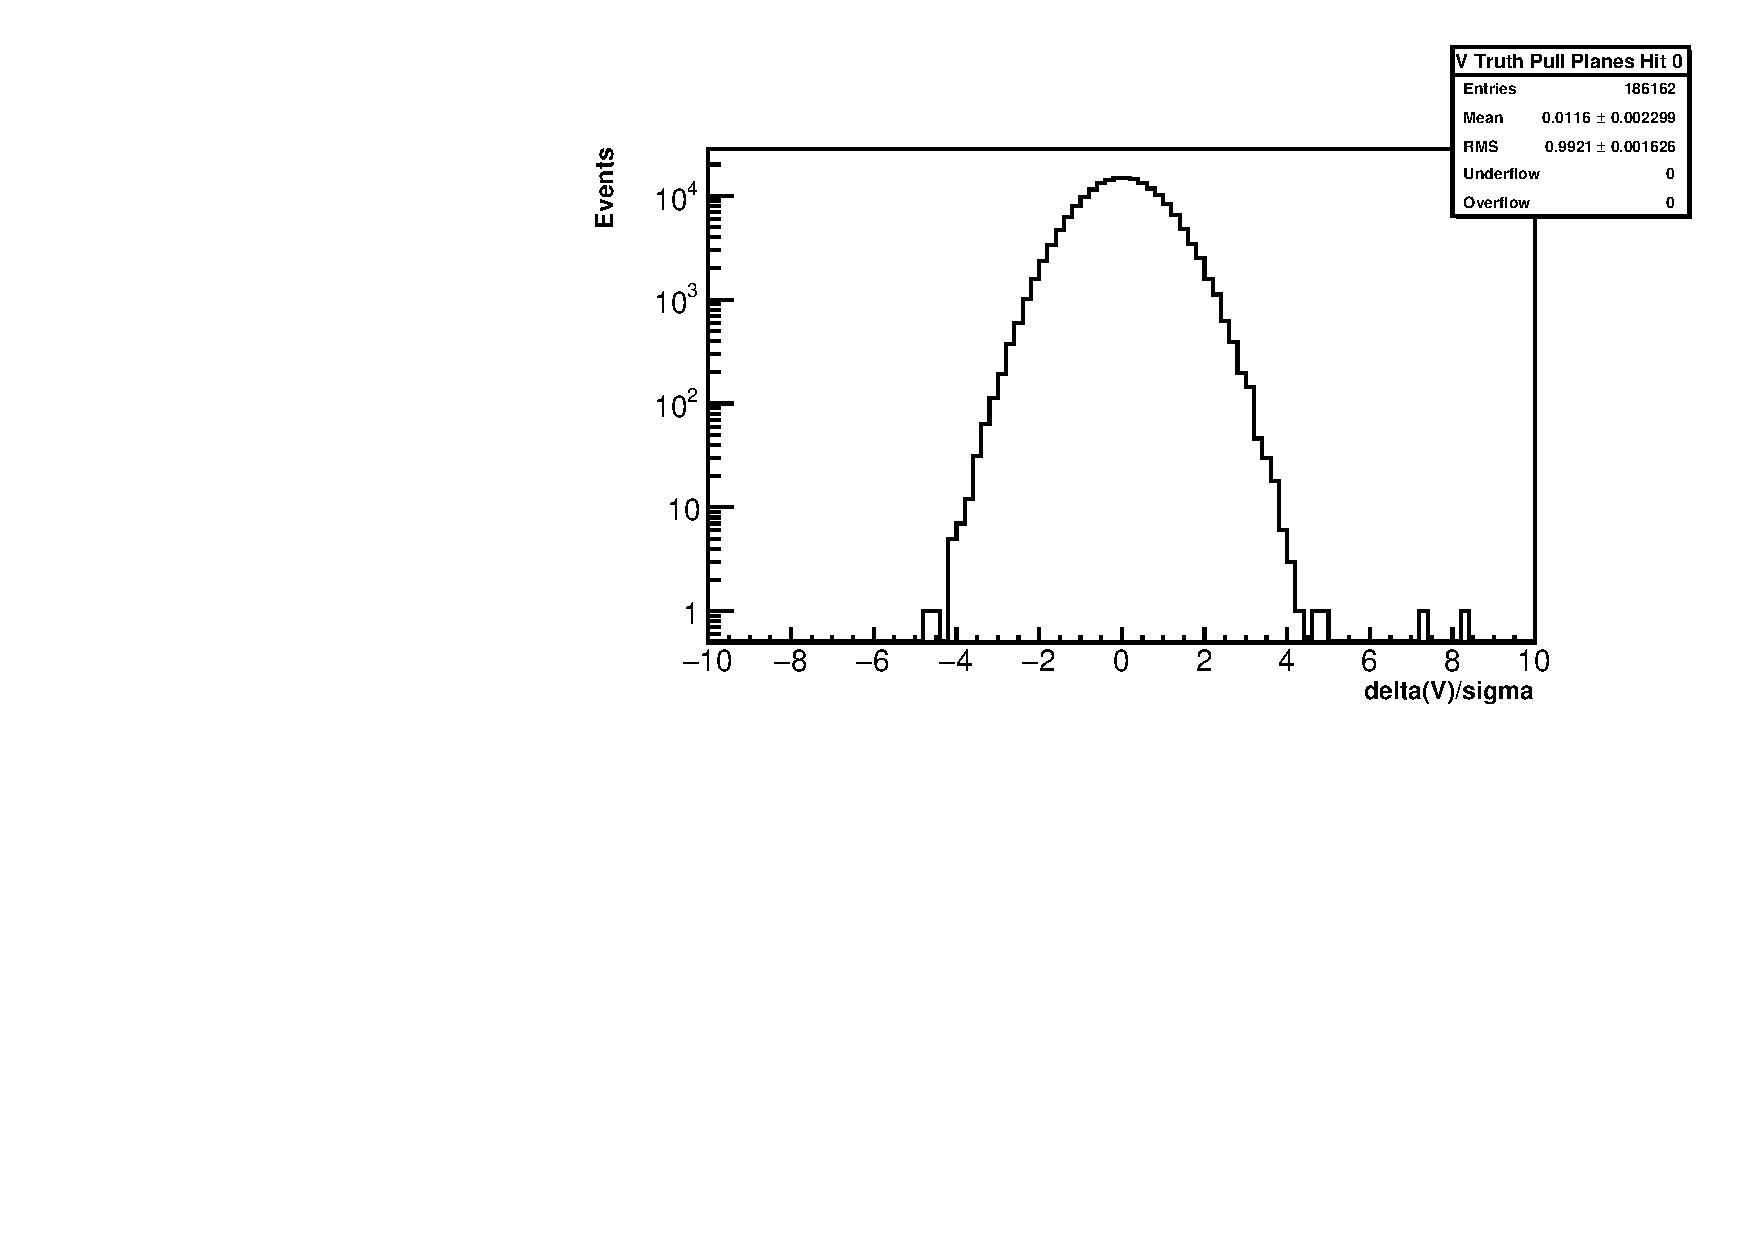
\includegraphics[width=1\textwidth]{VpullLog} 
        \caption{V truth pull on plane 0 for all tracks, log plot. Poor events can be seen as the distribution spreads out more towards the edges, with some under and overflows.}
    \end{subfigure}

    \caption{Number of iterations information.}
\end{figure}



\begin{figure}
    \centering
    \begin{subfigure}[]{0.6\textwidth}
        \centering
        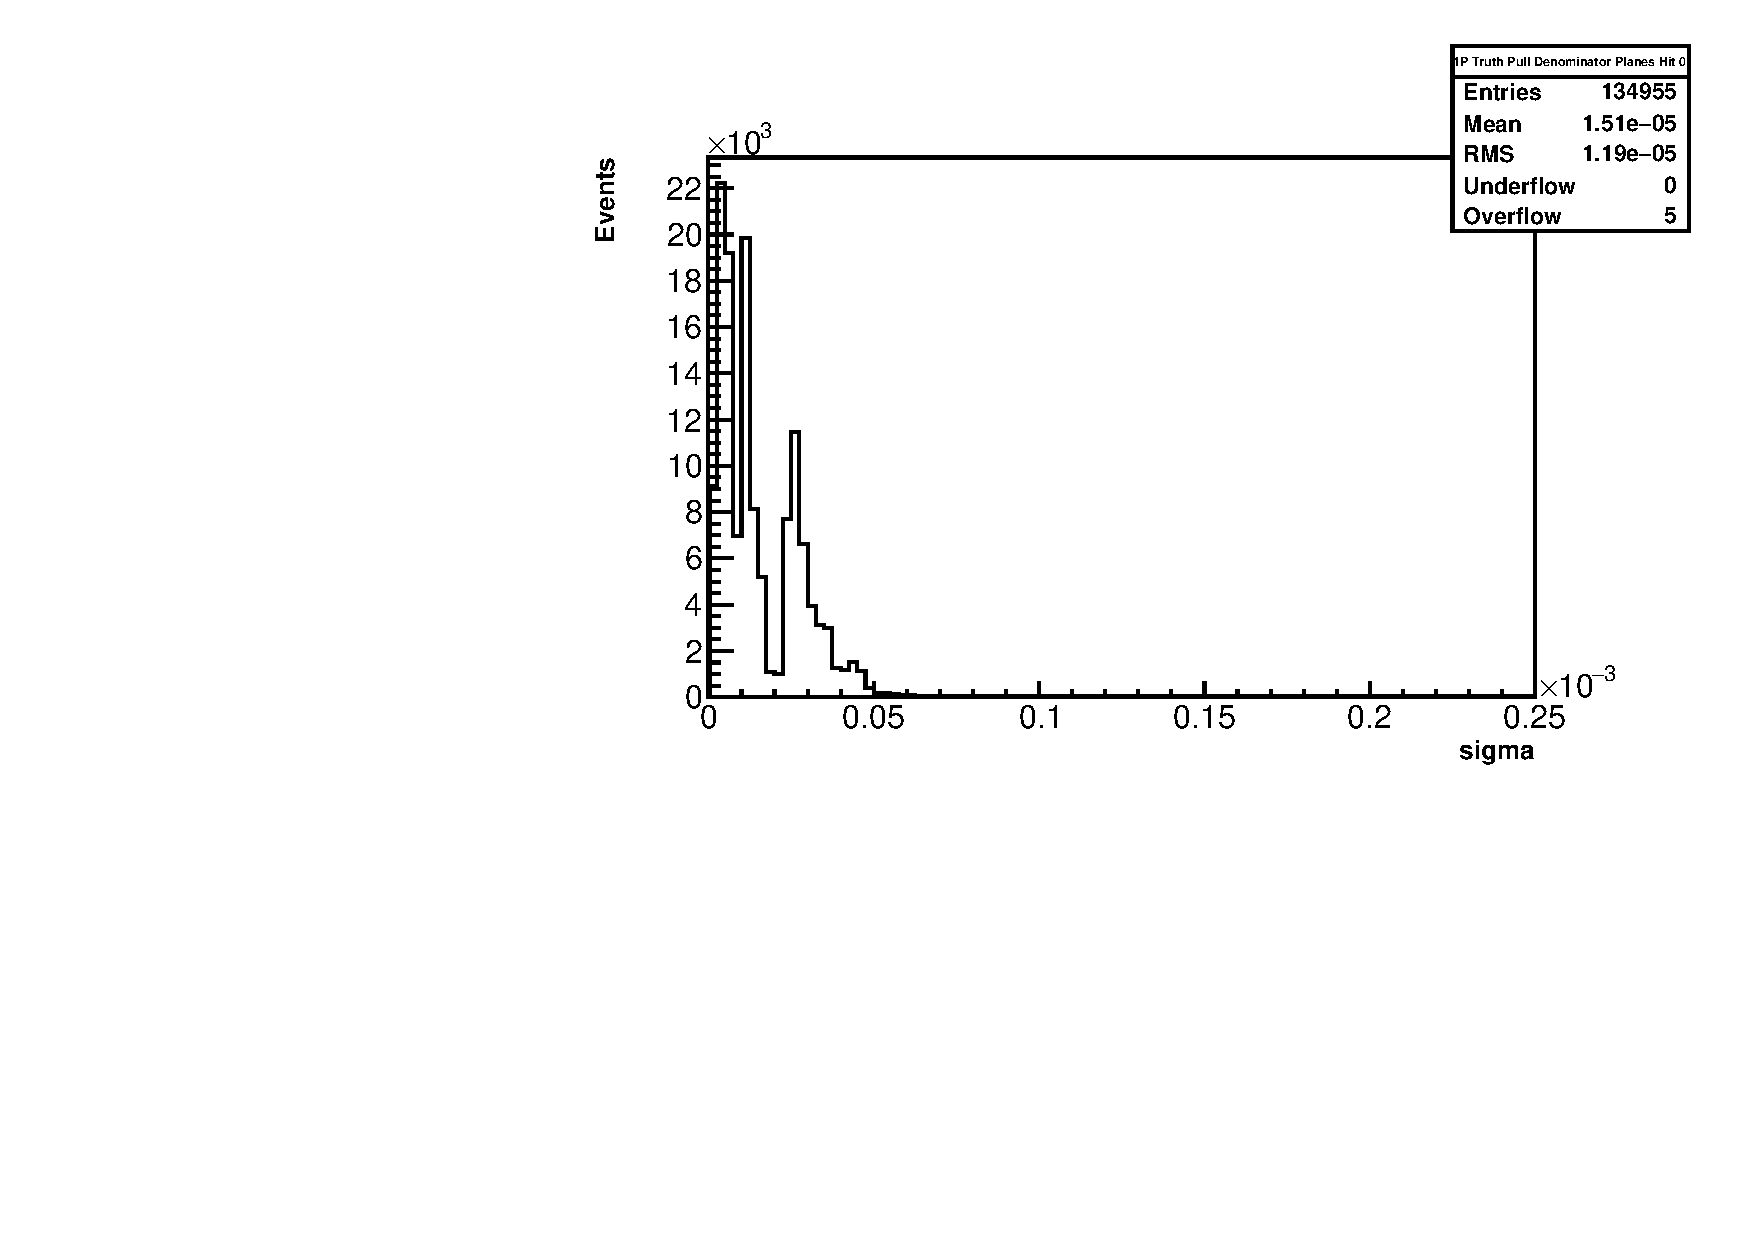
\includegraphics[width=1\textwidth]{1PpullDenom} 
        \caption{The error (denominator), in the 1/P pull. The different spikes corresponds to different numbers of planes hit, or different amounts of material passed through.}
    \end{subfigure}

    \begin{subfigure}[]{0.6\textwidth}
        \centering
        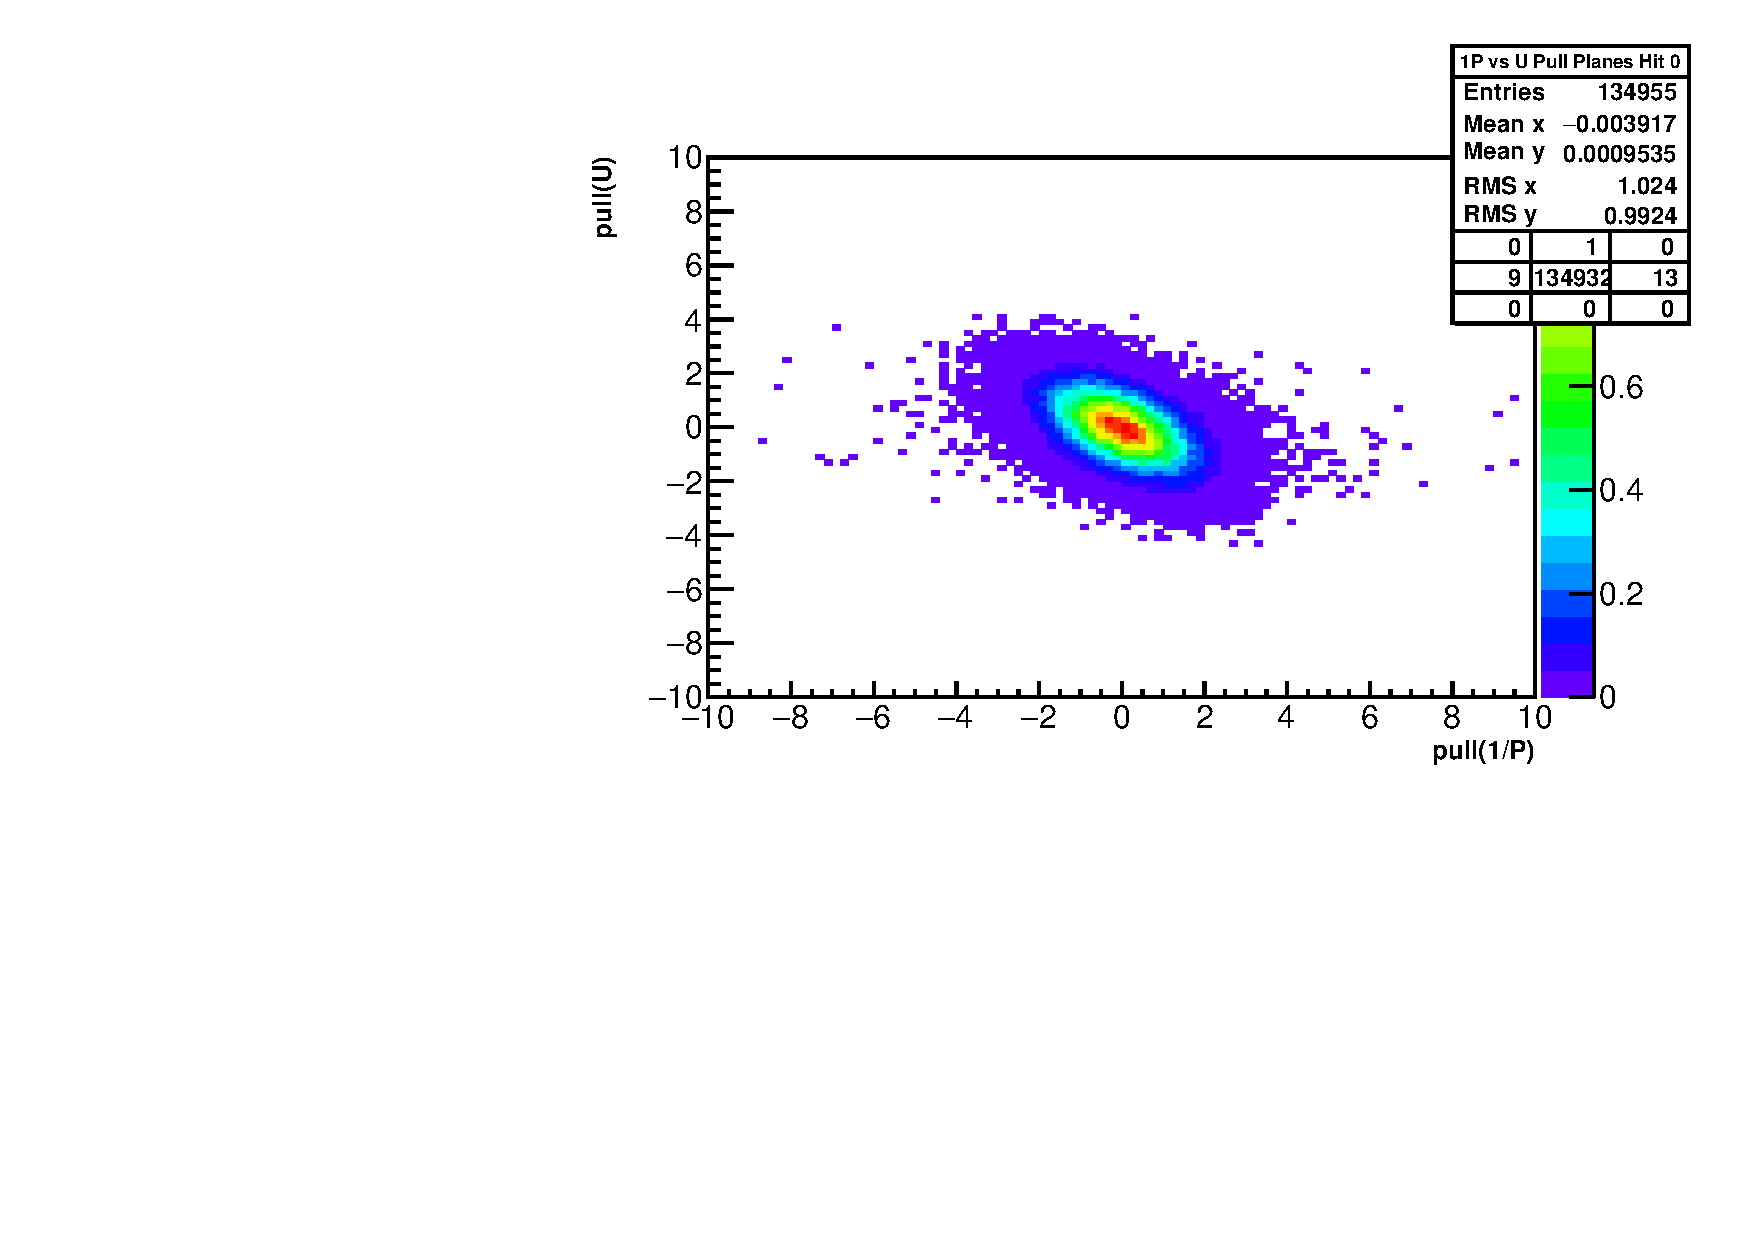
\includegraphics[width=1\textwidth]{1PpullVsUpull} 
        \caption{1/P pull vs U pull, the poor events can be seen spreading in a non-uniform way from the target.}
    \end{subfigure}
    
    \begin{subfigure}[]{0.6\textwidth}
        \centering
        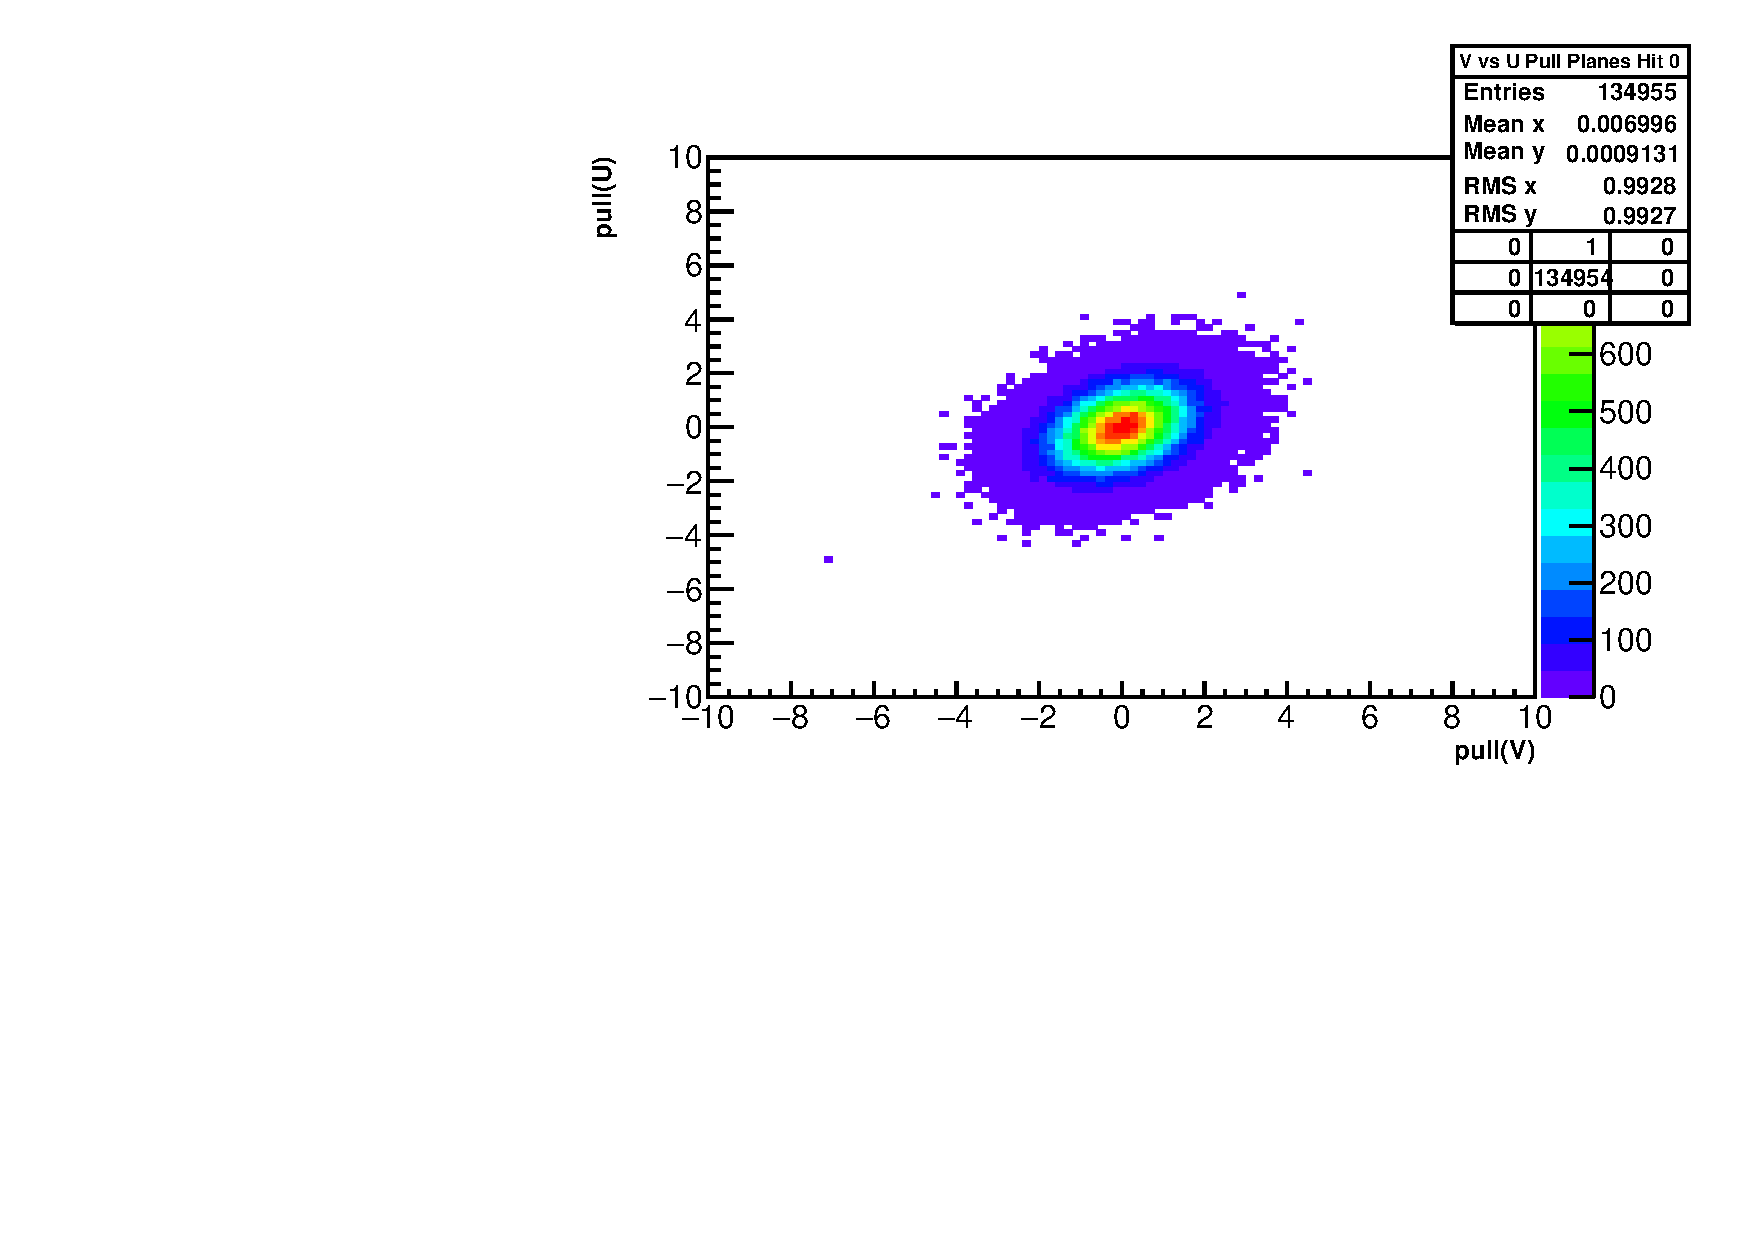
\includegraphics[width=1\textwidth]{UpullVsVpull} 
        \caption{U pull vs V pull.}
    \end{subfigure}

    \caption{Some various pull related plots.}
\end{figure}


\begin{figure}
    \centering
    \begin{subfigure}[]{0.6\textwidth}
        \centering
        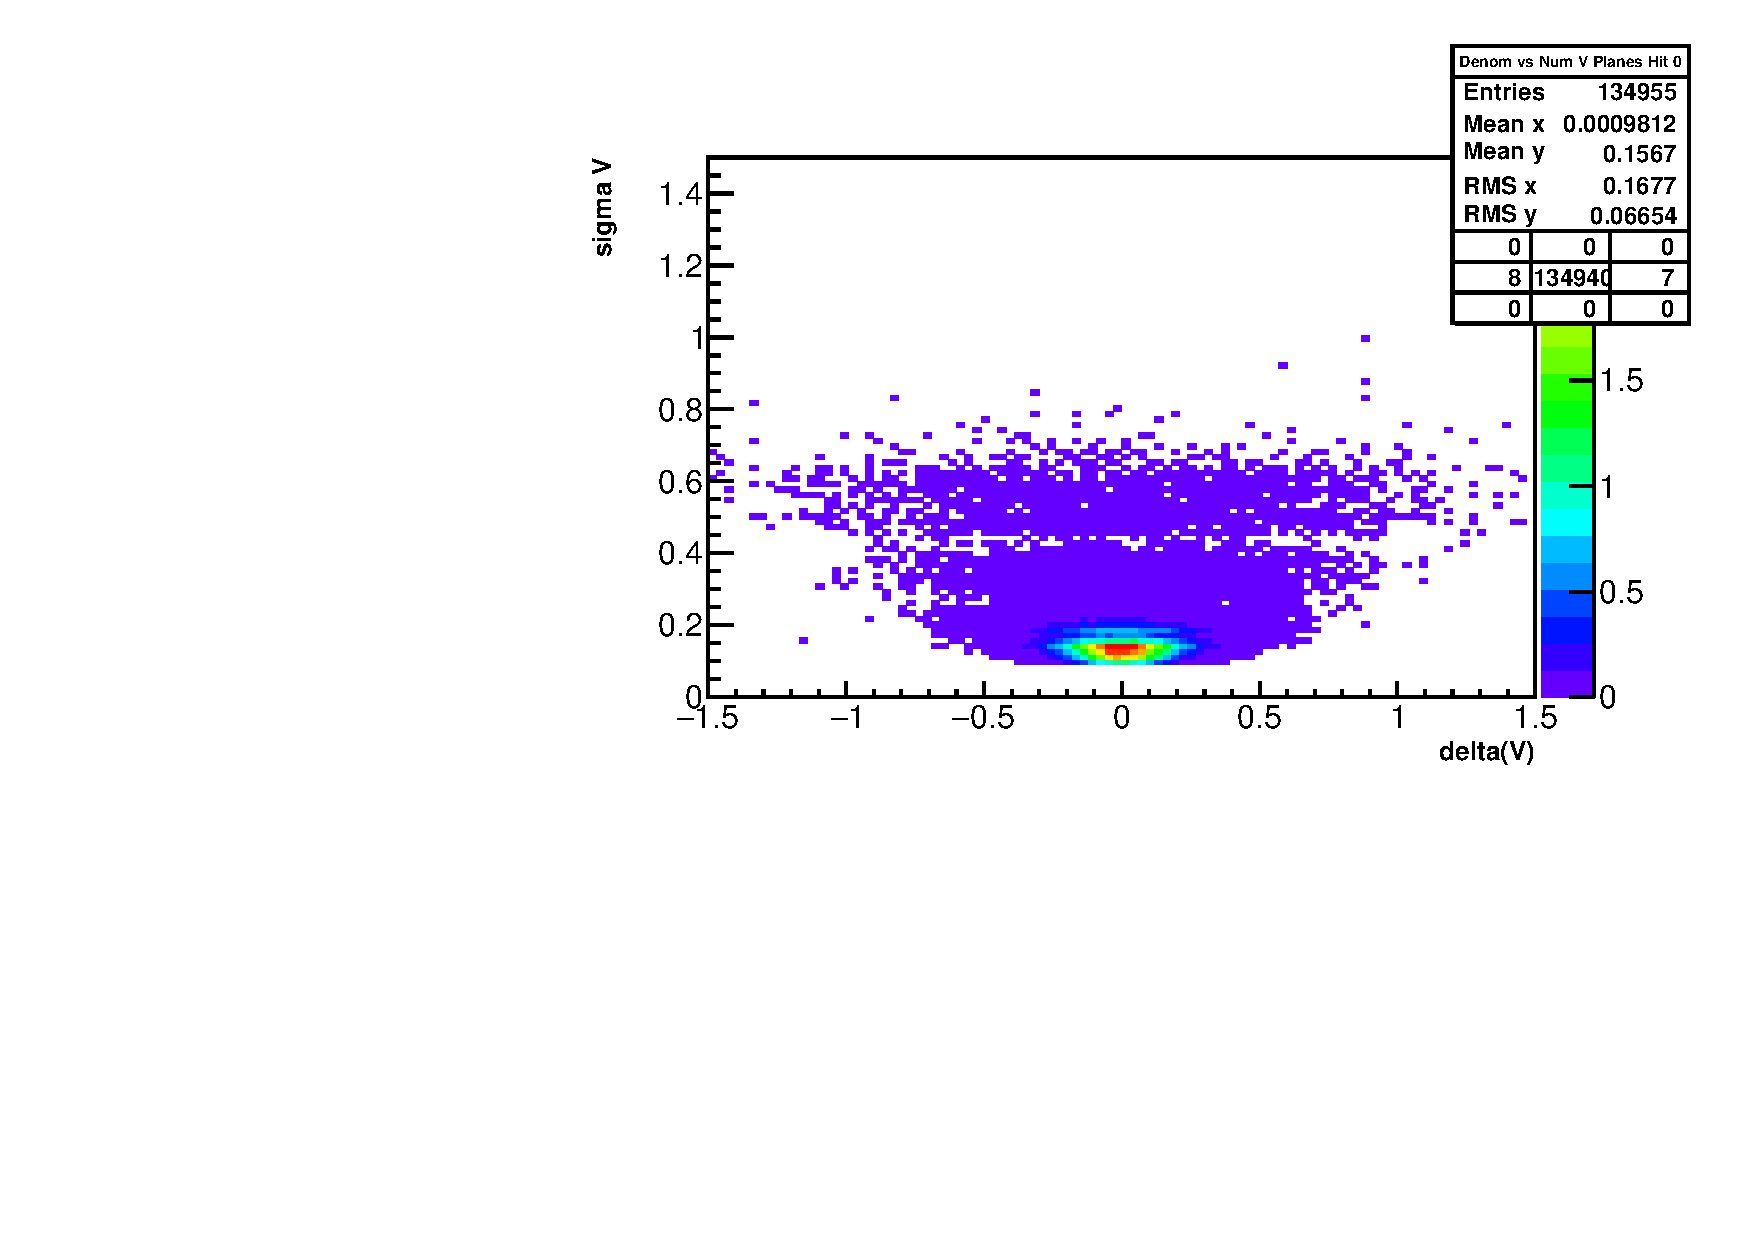
\includegraphics[width=1\textwidth]{VpullNumDenom} 
        \caption{The error in the V pull vs the residual in the V pull. The upper events are mostly comprised of tracks which hit less planes, leading to larger errors.}
    \end{subfigure}

    \begin{subfigure}[]{0.6\textwidth}
        \centering
        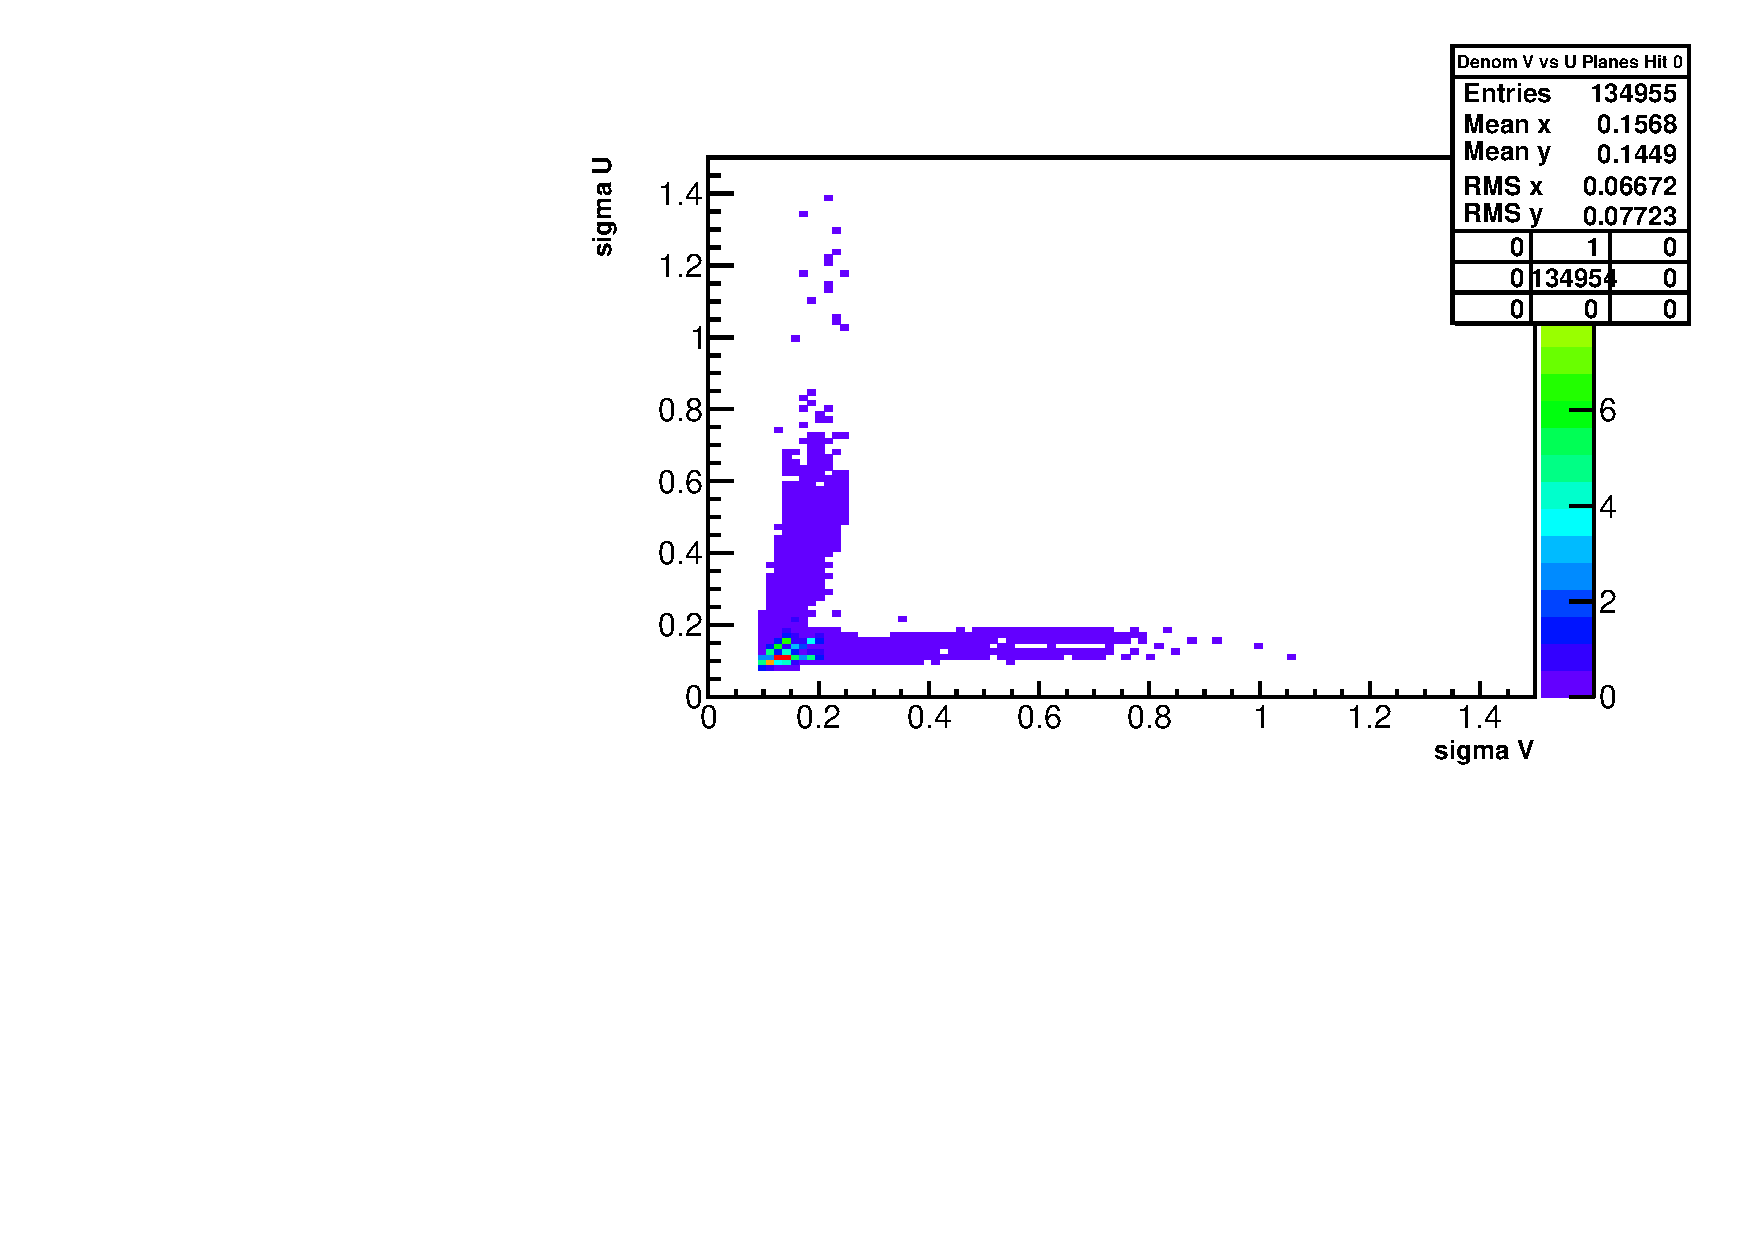
\includegraphics[width=1\textwidth]{DenomUV} 
        \caption{Error in U pull vs error in V pull, can be seen to be mostly uncorrelated within the fit.}
    \end{subfigure}
    
    \begin{subfigure}[]{0.6\textwidth}
        \centering
        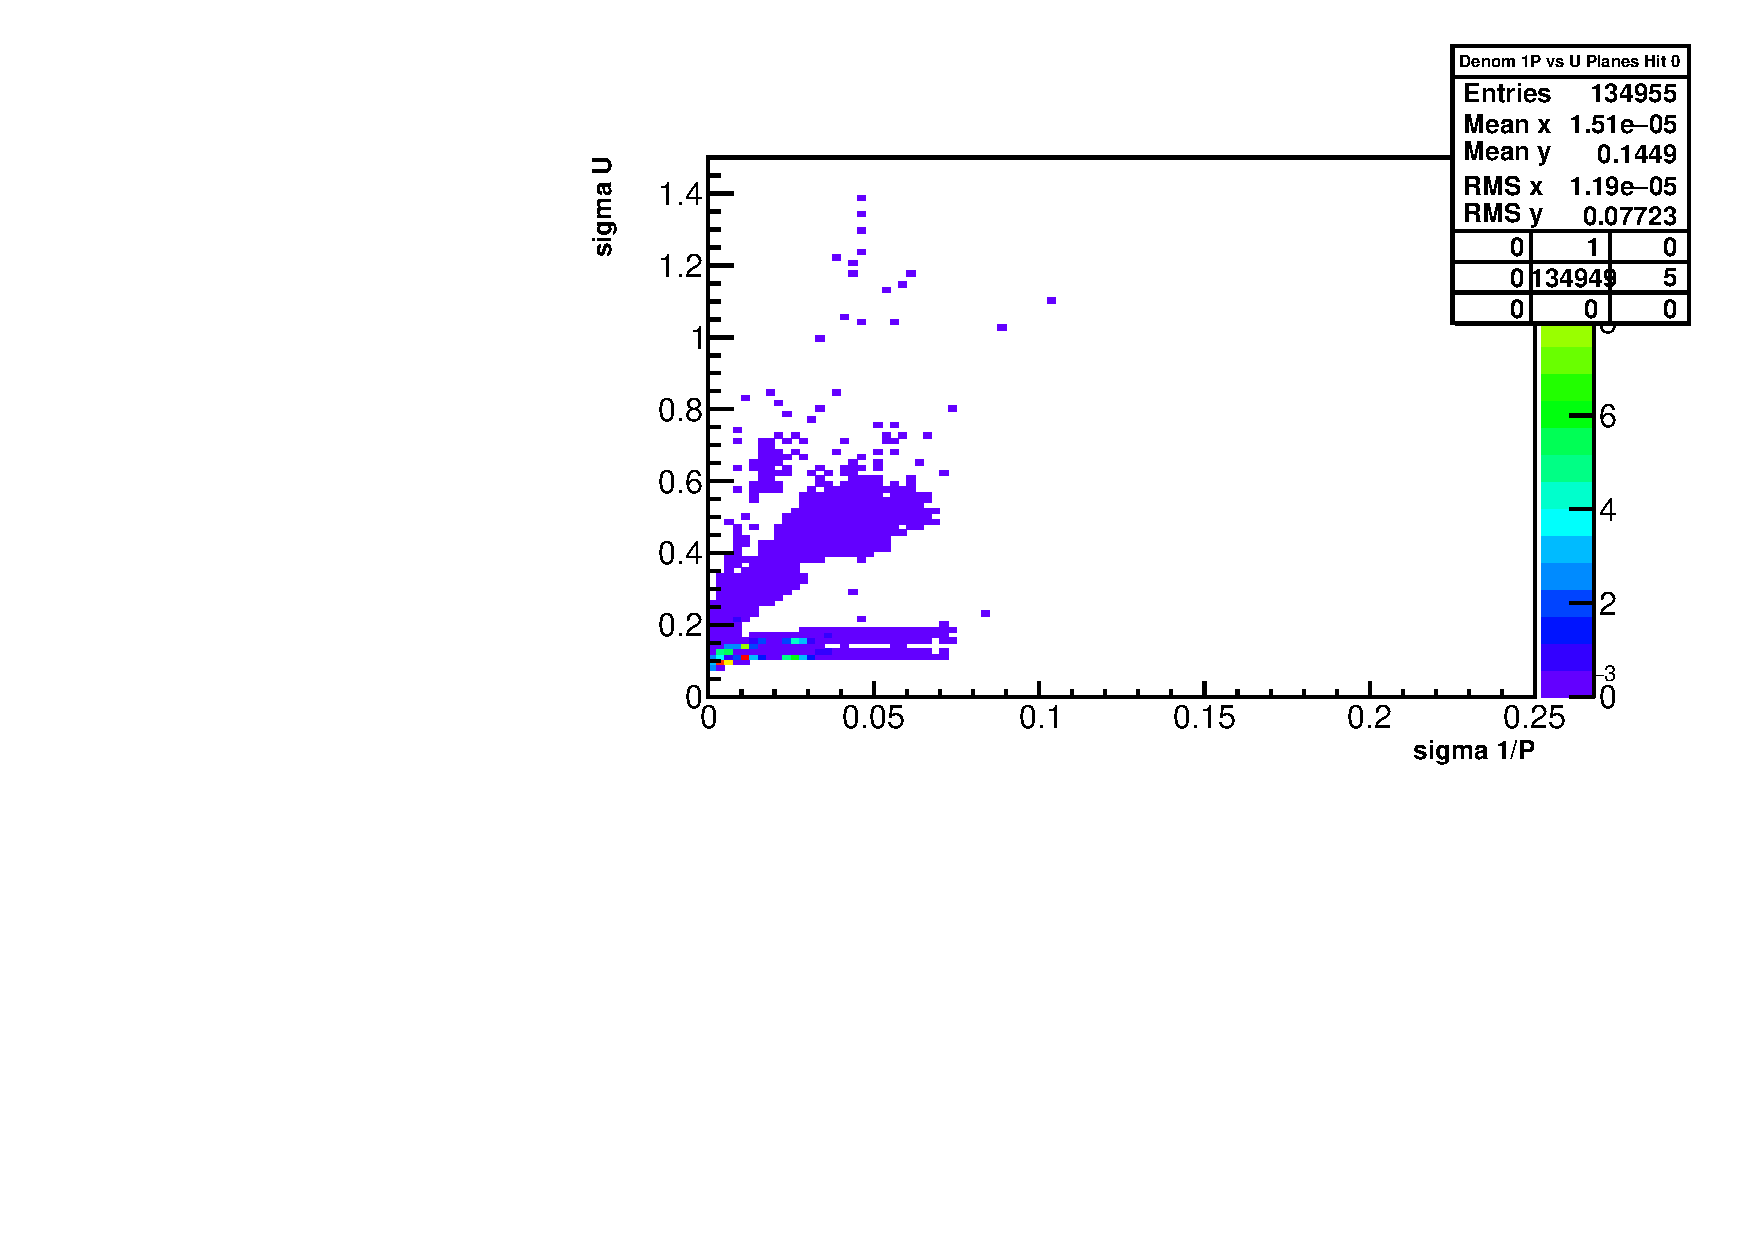
\includegraphics[width=1\textwidth]{Denom1PU} 
        \caption{Error in U pull vs error in 1/P pull. Some interesting structure is observed, that is not fully understood.}
    \end{subfigure}

    \caption{Some various pull related plots.}
\end{figure}



\begin{figure}
    \centering
    \begin{subfigure}[]{0.5\textwidth}
        \centering
        \includegraphics[width=1\textwidth]{meastruthrms} 
        \caption{RMS of measured - truth residuals, the input 150 $\mu$m smearing can be seen. Points on the X axis signify no measurement of that parameter on that plane.}
    \end{subfigure}

    \begin{subfigure}[]{0.5\textwidth}
        \centering
        \includegraphics[width=1\textwidth]{measpredrms} 
        \caption{RMS of measured - predicted residuals. There is an overall upside down parabolic shape to the distribution. A slight rise towards higher plane number indicates larger error due to increased material.}
    \end{subfigure}
    
    \begin{subfigure}[]{0.5\textwidth}
        \centering
        \includegraphics[width=1\textwidth]{predtruthrms} 
        \caption{RMS of predicted - truth residuals. There is an overall parabolic shape to the distribution, comprised of many parabolas. The RMS at the center of the fit is better than the edges since there are more measurements near the center. On individual planes, whatever that plane measured will have a better RMS, eg. plane 1 which is a U plane fits U better than V at that plane.}
    \end{subfigure}

    \caption{RMS of residual plots as a function of plane number for all events. Technically these should be split up according to number of planes hit, and the distance between the first and last hit in the fit, which would simplify and justify the shapes. See \href{http://gm2-docdb.fnal.gov:8080/cgi-bin/ShowDocument?docid=3813}{DocDB 3813} and \href{http://gm2-docdb.fnal.gov:8080/cgi-bin/ShowDocument?docid=6306}{DocDB 6306} to understand these plots.}
\end{figure}



\begin{figure}
    \centering
    \begin{subfigure}[]{0.6\textwidth}
        \centering
        \includegraphics[width=1\textwidth]{Pplane0} 
        \caption{Momentum magnitude from the fit at plane 0. X momentum distribution is very similar to this since most of the momentum is in the forward direction.}
    \end{subfigure}

    \begin{subfigure}[]{0.6\textwidth}
        \centering
        \includegraphics[width=1\textwidth]{Pyplane0} 
        \caption{Y momentum from the fit at plane 0. Bounded nicely by the measurement range of the detectors.}
    \end{subfigure}
    
    \begin{subfigure}[]{0.6\textwidth}
        \centering
        \includegraphics[width=1\textwidth]{Pzplane0} 
        \caption{Z momentum of the fit at plane 0. Some particles have outward radial momentum at the start of the fit (a negative value), and some inward, with all particles curving inward through the fit.}
    \end{subfigure}

    \caption{Momentum fit parameters on plane 0. Remember, the coordinate system is such that X is forward with the planes parallel, Y vertically up, and Z horizontal. The distributions here are very similar to truth as desired, which can be seen in the following truth residual plots.}
\end{figure}


\begin{figure}
    \centering
    \begin{subfigure}[]{0.55\textwidth}
        \centering
        \includegraphics[width=1\textwidth]{Xplane0} 
        \caption{X position from the fit at plane 0. Made up of individual delta functions since fits start at discrete 0 planes before each module. No tracks with the current Geane fitting starts at module 7 or 8 since such tracks don't hit enough planes to be fit.}
    \end{subfigure}

    \begin{subfigure}[]{0.55\textwidth}
        \centering
        \includegraphics[width=1\textwidth]{Yplane0} 
        \caption{Y position from the fit at plane 0. Bounded nicely by the measurement range of the detectors. The storage region width can be seen.}
    \end{subfigure}
    
    \begin{subfigure}[]{0.55\textwidth}
        \centering
        \includegraphics[width=1\textwidth]{Zplane0} 
        \caption{Z position of the fit at plane 0. There is an interesting spiky structure to the distribution, coming from how the detectors are staggered and shifted, and the incoming distribution of positrons. A larger negative value indicates a greater radial position. As a reminder this distribution is seen in truth as well.}
    \end{subfigure}

    \caption{Position fit parameters on plane 0. Remember, the coordinate system is such that X is forward with the planes parallel, Y vertically up, and Z horizontal. The distributions here are very similar to truth as desired, which can be seen in the following truth residual plots.}
\end{figure}


\begin{figure}
    \centering
    \begin{subfigure}[]{0.6\textwidth}
        \centering
        \includegraphics[width=1\textwidth]{P0TruthRes} 
        \caption{Momentum truth residual on plane 0. The distribution has an RMS of about 40 MeV.}
    \end{subfigure}

    \begin{subfigure}[]{0.6\textwidth}
        \centering
        \includegraphics[width=1\textwidth]{P0TruthResVsP} 
        \caption{Momentum truth residual on plane 0 vs P. As the momentum increase the spread in the residual increases, with the core staying relatively tight.}
    \end{subfigure}
    
    \begin{subfigure}[]{0.6\textwidth}
        \centering
        \includegraphics[width=1\textwidth]{Px0TruthRes} 
        \caption{X momentum truth residual on plane 0. Has an RMS of about 30 MeV. There are large tails in the distribution.}
    \end{subfigure}

    \caption{Momentum truth residuals on plane 0. Units are MeV. Most of the momentum and momentum spread is in the forward X direction. For real examination all of these plots should be split up according to the momentum of the track.}
\end{figure}


\begin{figure}
    \centering
    \begin{subfigure}[]{0.6\textwidth}
        \centering
        \includegraphics[width=1\textwidth]{P0TruthResRel} 
        \caption{Relative momentum truth residual on plane 0. There is about a 2\% resolution to the track fitting.}
    \end{subfigure}

    \begin{subfigure}[]{0.6\textwidth}
        \centering
        \includegraphics[width=1\textwidth]{P0TruthResVsPRel} 
        \caption{Relative momentum truth residual on plane 0 vs P. There is a tendency of the track fitting to overestimate the momentum of the track for some high momentum tracks.}
    \end{subfigure}
    
    \begin{subfigure}[]{0.6\textwidth}
        \centering
        \includegraphics[width=1\textwidth]{Px0TruthResRel} 
        \caption{X relative momentum truth residual on plane 0.}
    \end{subfigure}

    \caption{Relative momentum truth residuals on plane 0. For real examination all of these plots should be split up according to the momentum of the track.}
\end{figure}



\begin{figure}
    \centering
    \begin{subfigure}[]{0.6\textwidth}
        \centering
        \includegraphics[width=1\textwidth]{Py0TruthRes} 
        \caption{Y momentum truth residual on plane 0. The distribution has an RMS of about 4 MeV indicating the vertical momentum is pretty well measured, though tracks generally do not have much vertical momentum.}
    \end{subfigure}

    \begin{subfigure}[]{0.6\textwidth}
        \centering
        \includegraphics[width=1\textwidth]{Py0TruthResVsP} 
        \caption{Y momentum truth residual on plane 0 vs Py. There is a pretty tight core and some small corners in the distribution.}
    \end{subfigure}
    
    \begin{subfigure}[]{0.6\textwidth}
        \centering
        \includegraphics[width=1\textwidth]{Pz0TruthRes} 
        \caption{Z momentum truth residual on plane 0. Has an RMS of about 3 MeV, indicating the horizontal momentum is pretty well measured, though tracks generally do not have much horizontal momentum.}
    \end{subfigure}

    \caption{Momentum truth residuals on plane 0. Units are MeV. For real examination all of these plots should be split up according to the momentum of the track.}
\end{figure}

\clearpage

\begin{figure}
    \centering
    \begin{subfigure}[]{0.6\textwidth}
        \centering
        \includegraphics[width=1\textwidth]{X0TruthRes} 
        \caption{X position truth residual on plane 0. The distribution is a spike indicating that the X position of the fit is taken as known when fitting. Non-zero values indicate something is wrong with the fitting.}
    \end{subfigure}

    \begin{subfigure}[]{0.6\textwidth}
        \centering
        \includegraphics[width=1\textwidth]{Y0TruthRes} 
        \caption{Y position truth residual on plane 0. Has an RMS of about 740 $\mu$m as expected from simple geometry arguments coming from the 150 $\mu$m smearing. Even though particles do not curve much in Y, the straws don't measure the vertical position very well.}
    \end{subfigure}
    
    \begin{subfigure}[]{0.6\textwidth}
        \centering
        \includegraphics[width=1\textwidth]{Z0TruthRes} 
        \caption{Z position truth residual on plane 0. Has an RMS of about 135 $\mu$m as expected from simple geometry arguments coming from the 150 $\mu$m smearing. Better than the Y residual since both straws measure mostly in the horizontal direction, in spite of the fit having to deal with the curvature of the tracks.}
    \end{subfigure}

    \caption{Position truth residuals on plane 0. Units are mm. For real examination all of these plots should be split up according to the momentum of the track.}
\end{figure}







\end{document}
